\documentclass{article}

% if you need to pass options to natbib, use, e.g.:
%     \PassOptionsToPackage{numbers, compress}{natbib}
% before loading neurips_2026

% The authors should use one of these tracks.
% Before accepting by the NeurIPS conference, select one of the options below.
% 0. "default" for submission
\usepackage{neurips_2026}
% the "default" option is equal to the "main" option, which is used for the Main Track with double-blind reviewing.
% 1. "main" option is used for the Main Track
%  \usepackage[main]{neurips_2026}
% 2. "position" option is used for the Position Paper Track
%  \usepackage[position]{neurips_2026}
% 3. "eandd" option is used for the Evaluations & Datasets Track
 % \usepackage[eandd]{neurips_2026}
 % if you want to opt-in for a de-anomymized submission (not recommended, but OK):
 %\usepackage[eandd, nonanonymous]{neurips_2026}
% 4. "creativeai" option is used for the Creative AI Track
%  \usepackage[creativeai]{neurips_2026}
% 5. "sglblindworkshop" option is used for the Workshop with single-blind reviewing
 % \usepackage[sglblindworkshop]{neurips_2026}
% 6. "dblblindworkshop" option is used for the Workshop with double-blind reviewing
%  \usepackage[dblblindworkshop]{neurips_2026}

\usepackage{subcaption}

% After being accepted, the authors should add "final" behind the track to compile a camera-ready version.
% 1. Main Track
 % \usepackage[main, final]{neurips_2026}
% 2. Position Paper Track
%  \usepackage[position, final]{neurips_2026}
% 3. Evaluations & Datasets Track
 % \usepackage[eandd, final]{neurips_2026}
% 4. Creative AI Track
%  \usepackage[creativeai, final]{neurips_2026}
% 5. Workshop with single-blind reviewing
%  \usepackage[sglblindworkshop, final]{neurips_2026}
% 6. Workshop with double-blind reviewing
%  \usepackage[dblblindworkshop, final]{neurips_2026}
% Note. For the workshop paper template, both \title{} and \workshoptitle{} are required, with the former indicating the paper title shown in the title and the latter indicating the workshop title displayed in the footnote.
% For workshops (5., 6.), the authors should add the name of the workshop, "\workshoptitle" command is used to set the workshop title.
% \workshoptitle{WORKSHOP TITLE}

% "preprint" option is used for arXiv or other preprint submissions
 % \usepackage[preprint]{neurips_2026}

% to avoid loading the natbib package, add option nonatbib:
%    \usepackage[nonatbib]{neurips_2026}

\usepackage[utf8]{inputenc} % allow utf-8 input
\usepackage[T1]{fontenc}    % use 8-bit T1 fonts
\usepackage{hyperref}       % hyperlinks
\usepackage{url}            % simple URL typesetting
\usepackage{booktabs}       % professional-quality tables
\usepackage{amsfonts}       % blackboard math symbols
\usepackage{nicefrac}       % compact symbols for 1/2, etc.
\usepackage{microtype}      % microtypography
\usepackage{xcolor}         % colors
\usepackage{natbib}
\usepackage{amsmath}
\usepackage{graphicx}
\usepackage{subcaption}

% Note. For the workshop paper template, both \title{} and \workshoptitle{} are required, with the former indicating the paper title shown in the title and the latter indicating the workshop title displayed in the footnote. 
\title{Division of Labor Between Attention and SSM Layers in Hybrid Language Models}


% The \author macro works with any number of authors. There are two commands
% used to separate the names and addresses of multiple authors: \And and \AND.
%
% Using \And between authors leaves it to LaTeX to determine where to break the
% lines. Using \AND forces a line break at that point. So, if LaTeX puts 3 of 4
% authors names on the first line, and the last on the second line, try using
% \AND instead of \And before the third author name.


\author{%
  David S.~Hippocampus\thanks{Use footnote for providing further information
    about author (webpage, alternative address)---\emph{not} for acknowledging
    funding agencies.} \\
  Department of Computer Science\\
  Cranberry-Lemon University\\
  Pittsburgh, PA 15213 \\
  \texttt{hippo@cs.cranberry-lemon.edu} \\
  % examples of more authors
  % \And
  % Coauthor \\
  % Affiliation \\
  % Address \\
  % \texttt{email} \\
  % \AND
  % Coauthor \\
  % Affiliation \\
  % Address \\
  % \texttt{email} \\
  % \And
  % Coauthor \\
  % Affiliation \\
  % Address \\
  % \texttt{email} \\
  % \And
  % Coauthor \\
  % Affiliation \\
  % Address \\
  % \texttt{email} \\
}


\begin{document}


\maketitle
    

\begin{abstract}
TBD
\end{abstract}



\section{Introduction}
\label{sec:intro}

Hybrid language models combine standard transformer attention with state-space or linear-attention modules. These models are designed to improve efficiency while preserving strong language-modeling performance, and they are becoming increasingly common \citep{merrill2026olmohybridtheorypractice, qwen35blog, chandiramani2026nemotron}. However, it is still unclear how the different parts of hybrid models contribute to different tasks. In particular, when a hybrid model performs well, we do not know whether that behavior depends mostly on attention layers, SSM-style layers, or both working together.

This question matters because overall accuracy can hide how a model solves a task. A pure transformer and a hybrid model may reach similar accuracy while relying on different internal computations. A hybrid model may also perform better on some tasks while being more sensitive to the removal of specific layers. To understand hybrid models, we therefore need to look not only at whether they answer correctly, but also at which parts of the network are important for that behavior.

We study pure transformer and hybrid language models from the OLMo and Qwen families. We evaluate them on two task families: in-context retrieval and state tracking. The retrieval tasks ask models to recover information from the prompt, such as object colors, spatial relations, or simple counting facts. The state-tracking tasks ask models to maintain and update information across a sequence of operations.

We analyze these models using inference-time ablations. We first measure each model's normal task performance. Then, we remove individual layers or groups of module types during inference and measure how much performance changes. This gives a layer-wise sensitivity profile for each model and task, showing which parts of the network are most important for the model's behavior.
Our results show that simple in-context retrieval is largely solved across the models we test. Harder retrieval tasks, such as filtering, spatial reasoning, and arithmetic over retrieved objects, reveal larger differences between models. On state-tracking tasks, hybrid models often improve relative to pure transformers as the number or complexity of updates increases. However, the ablation results do not support a clean split where attention handles retrieval and SSM-style layers handle state tracking. Instead, different tasks depend on different parts of the network, and attention and SSM-style layers appear to work together.

Overall, our study shows that hybrid language models should not be understood only through aggregate accuracy or through a simple division of labor between module types. Their behavior depends on the task, the layer being ablated, and the interaction between attention and SSM-style components. These results provide a functional view of how hybrid models support retrieval and state tracking.

\section{Related Work}
\label{sec:rw}
Hybrid architectures are often explicitly engineered to divide computational roles. For example, \cite{Zhu2025} strictly partition processing into a transformer encoder and an SSM decoder, while \cite{ryoo2025generalizablerealtimeneuraldecoding} use attention for initial tokenization followed by SSM layers for fast inference. Other approaches enforce this division during training, such as using distillation to replace retrieval-heavy attention heads with efficient SSM layers \cite{bick2026retrievalawaredistillationtransformerssmhybrids}. While these designs prove the practical utility of mixed architectures, they leave open the question of how natively trained hybrids organically distribute computation.

Currently, most comparative evaluations of hybrids and pure transformers focus on aggregate performance, such as long-context modeling capabilities \cite{wornow2025contextcluesevaluatinglong}, leaving their internal mechanisms opaque. However, recent mechanistic work has begun opening the black box, demonstrating that pure transformers and pure SSMs solve identical tasks, using fundamentally different internal circuits \cite{arora2026mechanisticevaluationtransformersstate}.

Our work bridges the gap between these mechanistic insights and hybrid architecture analysis. We build directly upon recent ablation studies by \cite{borobia2026functionalcomponentablationreveals}, who establish that both attention and SSM components are critical to performance and that earlier layers exhibit higher sensitivity.

\textbf{TODO:} Max adds in the in context retrieval paper.

\section{Method}
\label{sec:method}

We study where task-relevant computation is localized in pure transformer and hybrid language models. Our approach uses inference-time functional ablations to measure how model behavior changes when specific components are removed.


\subsection{Layer-wise Ablations}
At inference time, we ablate a target module by replacing its forward pass with an identity mapping. 
This intervention removes the computation performed by that module while keeping the rest of the network unchanged. 
In our experiments, we perform layerwise ablations: for a decoder layer indexed by $\ell$, we ablate exactly one attention module at that layer and evaluate the resulting change in accuracy. 
In the pure transformer model, this always corresponds to removing one self-attention module. 
In the hybrid models, it corresponds to removing whichever attention module is active at layer $\ell$. 
By sweeping over all decoder layers, we obtain a layerwise sensitivity profile for each model and task.


\subsection{Component Ablations}
To understand macro-architectural dependencies, we perform component-level (or group) ablations. Rather than targeting individual layers, we simultaneously ablate all instances of a specific module class across the entire network. Specifically, we evaluate the removal of all standard multi-head self-attention modules (\texttt{self\_attn}) versus all state-space or linear attention modules (\texttt{linear\_attn}). 

Similar to our layer-wise approach, this is achieved by substituting the targeted modules with identity mappings during the forward pass. For pure transformer baselines, ablating self-attention removes the sequence routing mechanism entirely. For hybrid models, however, this targeted intervention allows us to isolate the specific computational division of labor. 

\subsection{Activation Patching}

\section{Experimental Setup}
\label{sec:exp}

\subsection{Models and Tasks}
\label{sec:models_and_tasks}
We evaluate six instruction-tuned language models from two distinct model families. The first family comprises \texttt{Olmo-3-7B-Instruct-SFT} \citep{olmo2025olmo3} and \texttt{Olmo-Hybrid-Instruct-SFT-7B} \citep{merrill2026olmohybridtheorypractice}. The second family consists of the Qwen models \citep{yang2025qwen3technicalreport}: \texttt{Qwen3-8B}, \texttt{Qwen3.5-9B}, \texttt{Qwen3.5-27B}, and \texttt{Qwen3-32B}. In our setup, \texttt{Olmo-3-7B-Instruct-SFT}, \texttt{Qwen3-8B}, and the larger \texttt{Qwen3-32B} serve as our pure transformer baselines. Conversely, \texttt{Olmo-Hybrid-Instruct-SFT-7B}, \texttt{Qwen3.5-9B}, and the larger-scale \texttt{Qwen3.5-27B} are evaluated as our hybrid models. This selection allows us to isolate the functional differences between pure transformer and hybrid architectures across both different model families and parameter scales.

We study these models on two broad task families: \textbf{in-context retrieval} and \textbf{state tracking}. The in-context retrieval family includes the \texttt{colored-objects} benchmark \citep{srivastava2023beyond} and \texttt{Needle-in-a-Haystack style} retrieval tasks \citep{needle-in-haystack}. The state-tracking family consists of tasks that probe whether models can maintain and update latent state across sequential operations, including the classical \texttt{entity tracking} task \citep{kim-schuster-2023-entity}, and a \texttt
{clinical sequence modeling} task \citep{wang2026handlinginterpretingmissingmodalities} that we formulate to identify the ability of decoder components to maintain and update internal representations of patient health states..

\subsection{Evaluation Protocol and Metrics for the In Context Retrieval Task}\label{sec:eval}

\paragraph{In-Context Retrieval Task}
% TODO Add examples
% Add logit lens results?
We evaluate in-context retrieval using the Colored Objects benchmark, which tests whether a model can extract object attributes and simple relations from a short textual context. Each example describes a set of colored objects and is followed by a query whose answer must be recovered directly from the prompt. 
We report both baseline performance and layerwise ablation results.

The benchmark contains multiple subtask types that probe different forms of retrieval. 
In the \texttt{color} subtask, the model must identify the object associated with a queried color. 
In the \texttt{what\_color} subtask, the model must identify the color associated with a queried object. 
In the \texttt{yes\_no\_color} subtask, the model is given a candidate object-color pairing and must determine whether it is correct, 
producing a binary yes/no response. In the \texttt{spatial} subtask, the model must answer a query about the relative arrangement or position of objects described in the prompt. 
In the \texttt{arithmetic} subtask, the model must answer a retrieval query that additionally requires a small amount of compositional or counting-based reasoning over the objects in context. 
These subtasks allow us to compare performance across closely related retrieval settings that vary in query form and response structure.

To control for variation in prompt complexity, we balance evaluation by the number of objects mentioned in the prompt. Specifically, we group examples by object count and sample equally from each group. 
For each subtask, we use the largest balanced subset permitted by the smallest object-count group, 
so that comparisons are not driven by differences in prompt-length distributions across subtasks.

Because the evaluated models are run in chat mode, we use a chat-style prompting format for all Colored Objects experiments. Model outputs are generated greedily with a maximum generation length of 16 tokens. 
Performance is measured using accuracy, where a prediction is counted as correct if the parsed model output matches a gold target answer.
The same evaluation procedure is used for both the baseline runs and the corresponding layerwise ablation experiments.


\subsection{Evaluation Protocol and Metrics for the Entity Tracking Task}

\paragraph{Entity Tracking Task} We use the \emph{Boxes} task from~\citet{kim-schuster-2023-entity}. Each example consists of a short narrative describing an initial inventory of $N$ boxes, each containing at most $M$ objects, with an expected number of $K$ objects, followed by a sequence of operations drawn from $\{\texttt{move}, \texttt{remove}, \texttt{put}\}$. The model is then asked to predict the contents of a single queried box after all operations have been applied.

A prototypical 6-box, 3-operation example is shown below:

\begin{quote}
\small
\texttt{Box 0 contains the tea, Box 1 contains the file, Box 2 contains the pot, Box 3 contains the flower, Box 4 contains the fan, Box 5 contains the tissue. Remove the flower from Box 3. Put the brain into Box 1. Move the fan from Box 4 to Box 2. \ldots\, Box 4 contains the}
\end{quote}

To study how model performance varies with the number of operations, we fix the task setting to $N=6$ boxes, with $M=3$ and $K=2$. We generate 200 instances for each number of operations applied to the queried box, with $n_{\mathrm{op}} \in \{0,1,2,3,4,5\}$. To study the effect of the number of boxes, we use the same instance-generation procedure while varying $N \in \{2,3,4,5,6\}$.

Because all tested models are instruction-tuned, we adapt the task into a short one-turn conversation template. The initial inventory and sequence of operations are provided in the user turn, while the queried box is provided as a prefix in the assistant turn. We then allow the model to generate freely using greedy decoding until it reaches an EOS token. Since the outputs are free-form, we use a string-matching parser to extract the predicted set of items in the queried box. We compare the extracted set against the ground-truth set and report exact-match accuracy, assigning a score of 1 only when the entire predicted set matches the ground truth and 0 otherwise.

\paragraph{Minimal Pair Generation for Activation Patching} 
Activation patching requires \emph{paired} examples: a \emph{clean} input whose final-token representation supports the correct answer, and a \emph{corrupt} input that is structurally identical but has a different answer. Na\"ively pairing arbitrary examples is problematic because the resulting prompts may have different lengths, making position-level patching ill-defined. To avoid this issue, we first generate abstract \emph{skeletons} that fix the full causal structure of an example: the number of boxes ($N=6$), the sequence of operation types, the boxes involved in each operation, and the queried box. Each skeleton can then be instantiated with different object names while preserving the same underlying state-transition structure.

Crucially, object positions in the skeleton are represented by symbolic slots (\texttt{slot\_0}, \texttt{slot\_1}, \ldots) rather than concrete object names. For each skeleton, we sample two independent \emph{object-name assignments} from a curated vocabulary. Each assignment maps slots to concrete object strings with matched token length. When a fast tokenizer is available, we enforce this constraint directly: any instantiated variant whose token count differs from the skeleton's canonical token count is discarded. This procedure yields clean/corrupt pairs with identical \texttt{input\_ids} structures, allowing activations to be patched at corresponding positions without sequence misalignment. See Figure~\ref{fig:skeleton_and_slots} for an example.

\begin{figure}
    \centering
    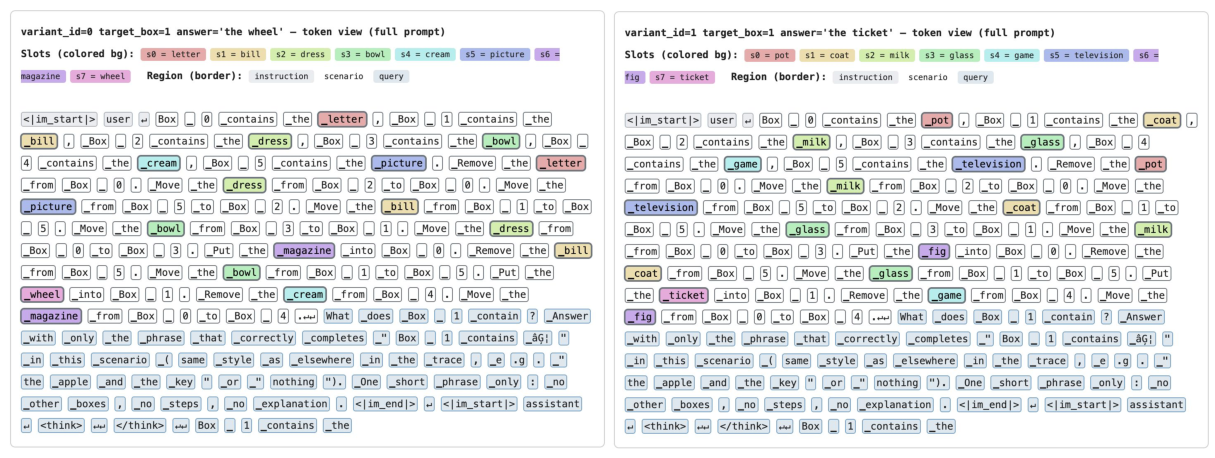
\includegraphics[width=1\linewidth]{assets//img/skeleton_and_slots.pdf}
    \caption{Example of two variants of the same skeleton (tokenized with Qwen tokenizer).}
    \label{fig:skeleton_and_slots}
\end{figure}

For this set of experiments, we restrict the queried box to contain exactly one object, so that each example has a single clean answer token and a single corrupt answer token. Let $a_c$ denote the clean answer token and $a_{\tilde{c}}$ denote the corrupt answer token. For a model run with final-token logits $\ell$, we define the logit difference as
\[
\Delta(\ell) = \ell(a_c) - \ell(a_{\tilde{c}}).
\]
We compute this quantity for the clean run, the corrupt run, and each patched run, yielding $\Delta_{\mathrm{clean}}$, $\Delta_{\mathrm{corrupt}}$, and $\Delta_{\mathrm{patch}}$, respectively. We report the normalized patched logit difference as
\[
\frac{\Delta_{\mathrm{patch}} - \Delta_{\mathrm{corrupt}}}
{\Delta_{\mathrm{clean}} - \Delta_{\mathrm{corrupt}}},
\]
which measures the extent to which the patch restores the clean behavior relative to the corrupt baseline.



\section{Results}
\label{sec:results}

\subsection{In-Context Retrieval}

\subsubsection{Behavioral Results}
Figure~\ref{fig:baselines1} shows that the three subtasks in the main text differ substantially in difficulty. Performance on \texttt{what\_color} is near ceiling for all four models, 
and performance on \texttt{yes\_no\_color} is also uniformly high. 
In contrast, \texttt{neither\_color} is much harder and shows the clearest separation between models, 
with stronger architectures achieving substantially higher accuracy. 
Figure~\ref{fig:baselines2} extends this comparison to the remaining two subtasks, \texttt{spatial} and \texttt{arithmetic}, which are also considerably more difficult than \texttt{what\_color} and \texttt{yes\_no\_color}. Taken together, these results show that simple attribute retrieval is largely solved by all models we evaluate, whereas more demanding retrieval settings remain strongly model-dependent.


\begin{figure}[t]
    \centering
    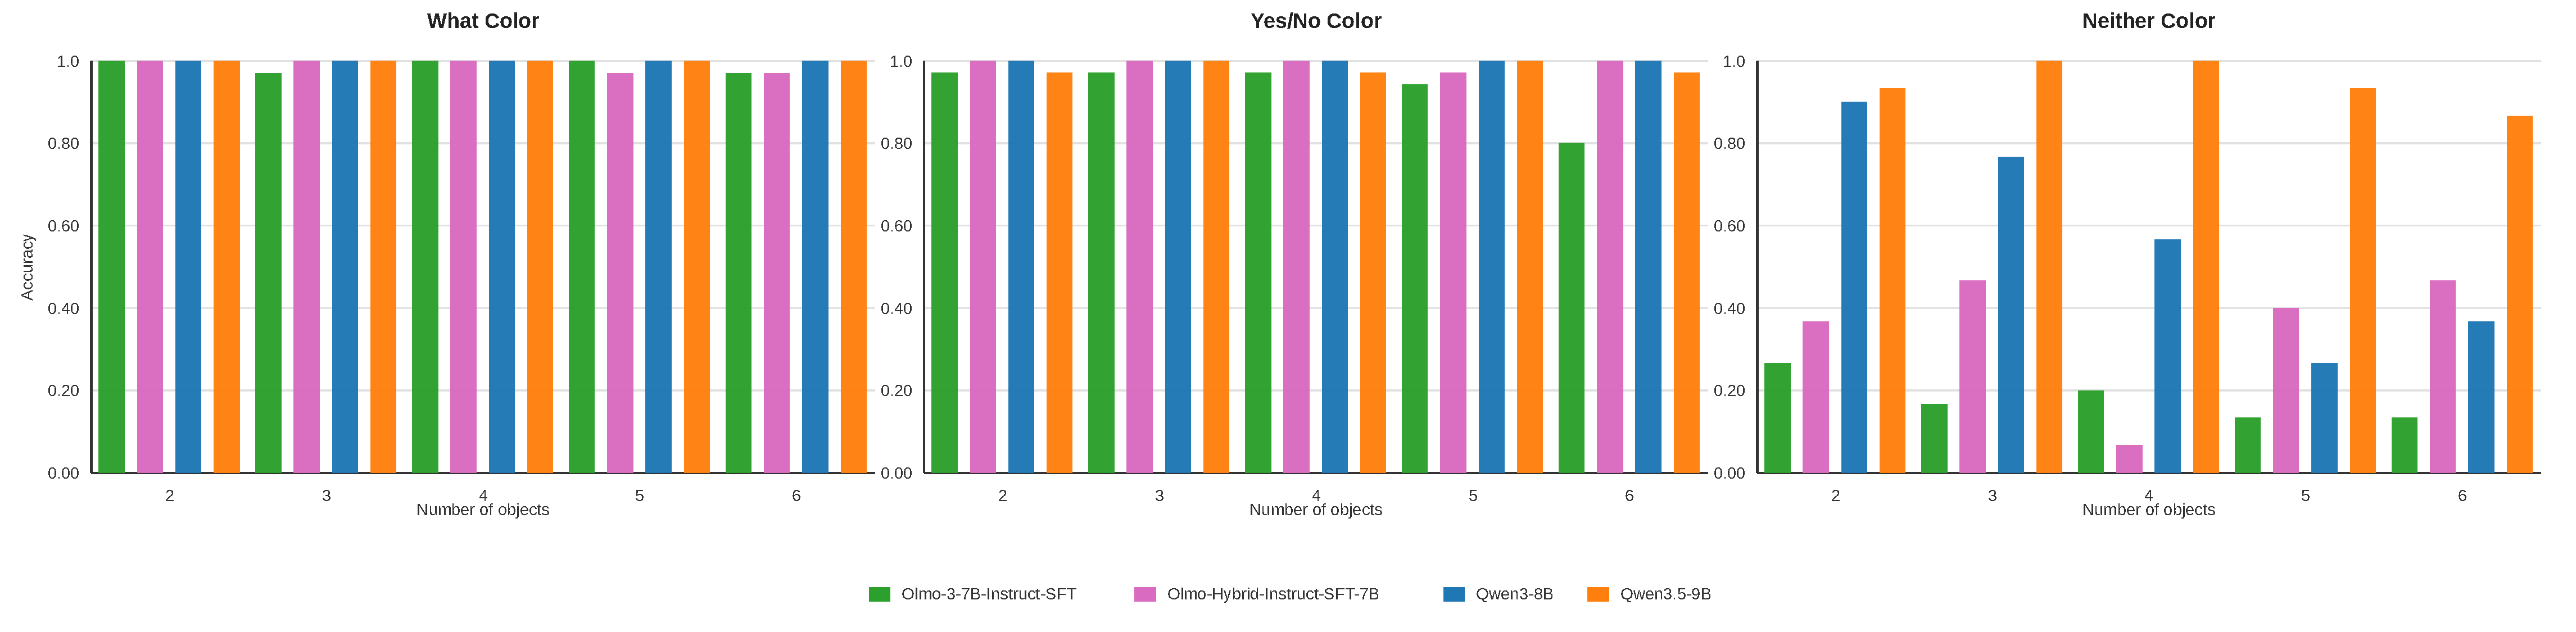
\includegraphics[width=\linewidth]{assets/colored_objects/baselines_top_row.pdf}
    \caption{Baseline accuracy on the Colored Objects subtasks \texttt{what\_color}, \texttt{yes\_no\_color}, and \texttt{neither\_color}. The x-axis shows the number of objects in the prompt, and the y-axis shows accuracy. Bars compare Olmo-3-7B-Instruct-SFT, Olmo-Hybrid-Instruct-SFT-7B, Qwen3-8B, and Qwen3.5-9B within each object-count bin.}
    \label{fig:baselines1}
\end{figure}


\subsubsection{Layer-wise Ablation Results}

Figure~\ref{fig:ablations1} shows that the three main-text subtasks also differ in their sensitivity to layer ablation. Ablations have relatively limited effect on \texttt{what\_color} and \texttt{yes\_no\_color}, especially for the stronger models, consistent with their high baseline accuracy. By contrast, \texttt{neither\_color} is much more sensitive to ablation, with larger performance drops concentrated at particular layers. Comparing the pure transformer and hybrid Olmo models specifically, the hybrid model is generally more robust on these subtasks: it matches the pure transformer on \texttt{what\_color}, outperforms it on \texttt{yes\_no\_color}, and substantially outperforms it on \texttt{neither\_color}, while also showing less severe degradation across many ablated layers. At the same time, the hybrid model often collapses when a single early layer is ablated, suggesting that although it is usually stronger overall, it can rely more heavily on specific early-layer computations. Figure~\ref{fig:ablations2} shows that \texttt{spatial} and \texttt{arithmetic} are likewise more ablation-sensitive than the easiest subtasks. Here again, the hybrid model is stronger than the pure transformer on \texttt{spatial}, though \texttt{arithmetic} is an exception where the pure transformer attains higher baseline accuracy. Overall, the ablation results suggest that the computations required for the harder retrieval subtasks are more fragile and more localized, and that the hybrid architecture is usually, though not uniformly, more robust than its pure-attention counterpart.

\begin{figure}[t]
    \centering
    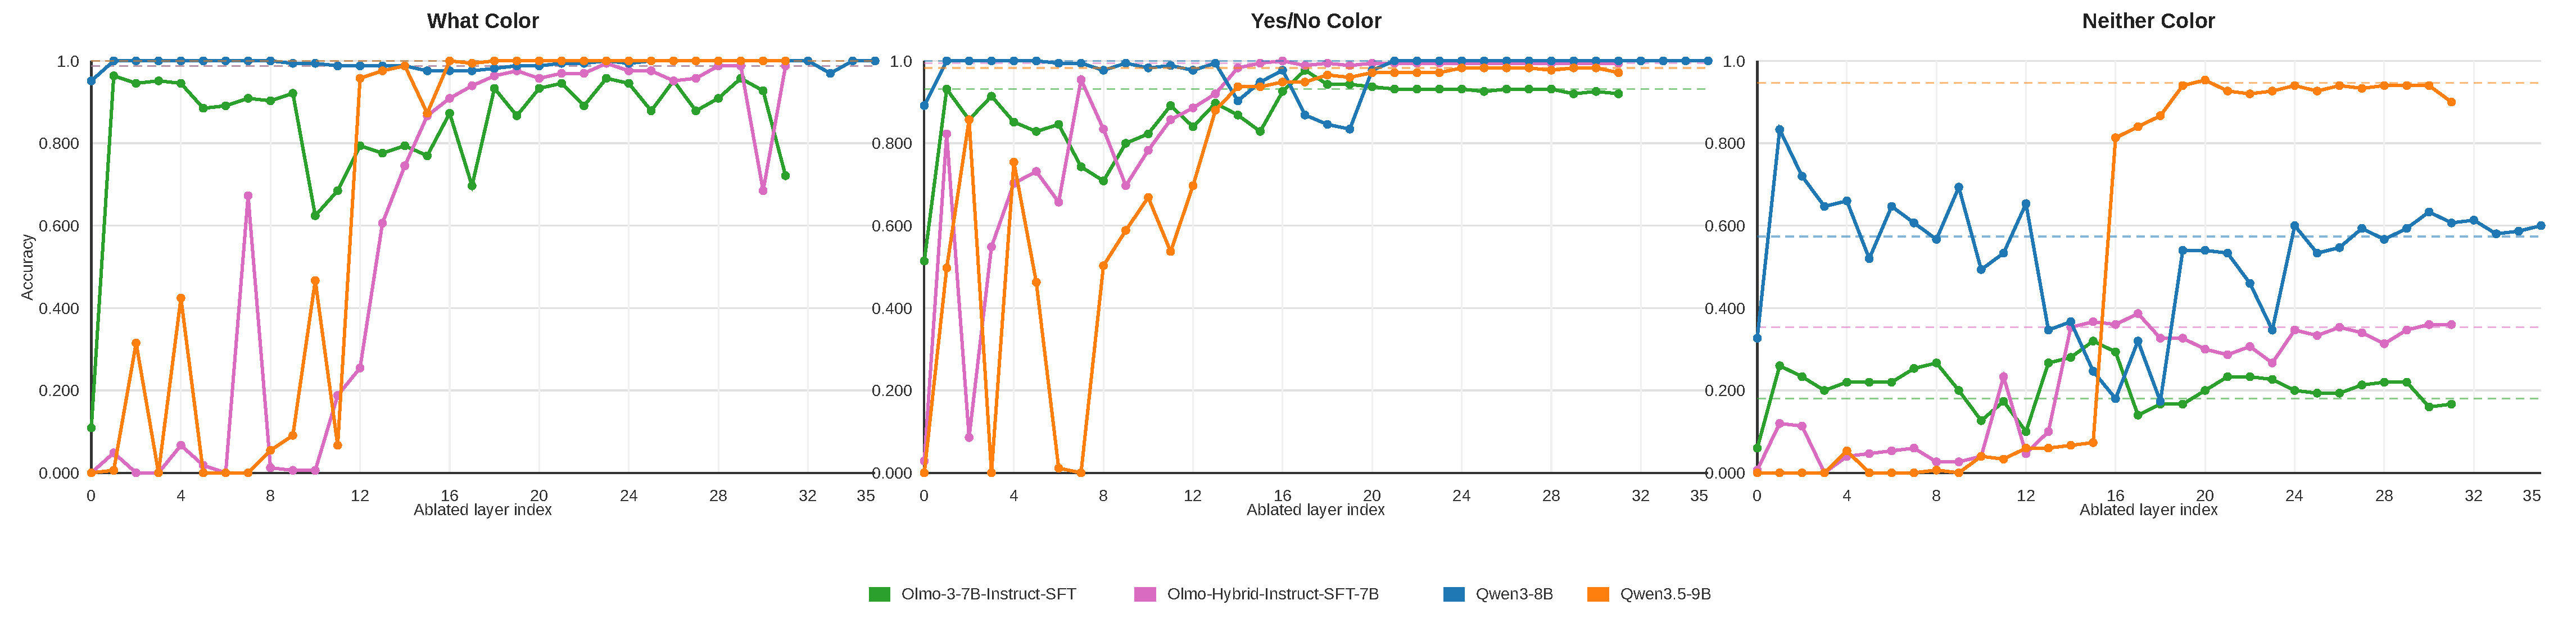
\includegraphics[width=\linewidth]{assets/colored_objects/ablations_top_row.pdf}
    \caption{Per-layer ablation accuracy on the Colored Objects subtasks \texttt{what\_color}, \texttt{yes\_no\_color}, and \texttt{neither\_color}. The x-axis shows the index of the ablated layer, and the y-axis shows accuracy after ablation. Dashed horizontal lines indicate each model's baseline accuracy without ablation.}
    \label{fig:ablations1}
\end{figure}

\subsubsection{Logit Lens Analysis}
We use logit lens to ask when, across depth, the correct answer becomes decodable from the model’s final-token representation.
At each decoder layer, we project the hidden state at the final prompt position through the model’s final normalization and output head to obtain vocabulary logits.
We then restrict scoring to the example’s candidate answer set and measure the log-probability assigned to the gold answer.
Our main logit-lens metric is the mean gold log-probability by probe layer, and we additionally compute choice-restricted accuracy and mean gold rank. In the ablated setting, this analysis also identifies which layers are causally important for constructing or maintaining the representation that supports the correct answer.


\subsection{State Tracking}

\subsubsection{Behavioral Results}

\paragraph{Entity Tracking} We first compare pure-attention transformer models with similarly sized hybrid models on the entity tracking task across different number of operations in this task. Figure~\ref{fig:entity_tracking_nbox6_comparison} reports model prediction set accuracy as a function of the number of operations applied to the queried box. Overall, hybrid models become relatively stronger as the number of queried-box operations increases. In the Qwen comparisons, hybrid models generally match or outperform their pure-attention counterparts at higher values of numops, consistent with the hypothesis that hybrid architectures may better support iterative state updates.  One notable observation appears in the OLMo comparison at numops = 0, where the OLMo hybrid model substantially underperforms the pure-attention OLMo model. This condition does not require tracking any state changes: because no operation has been applied to the queried box, the model only needs to retrieve the box’s initial state from context. The performance drop may therefore suggest that the OLMo hybrid model is weaker at pure in-context retrieval, a setting where full-attention transformers are theoretically better suited. We also investigate the effect of number of boxes to the comparative state-tracking advantages of hybrid models. 

Next, Figure~\ref{fig:entity_tracking_boxes_operations_comparison} compares pure-attention transformers and similarly sized hybrid models as the number of boxes and type of operations vary. Across all three model-family comparisons, hybrid models consistently outperform their pure-attention counterparts, and this advantage generally persists across all box counts. Performance decreases as the number of boxes increases, suggesting that the task becomes harder as the state space grows. However, the relative gap between hybrid and pure-attention models remains visible, especially when examples include \texttt{move} operations. Since \texttt{move} requires simultaneously removing an object from one box and adding it to another, this operation imposes a stronger state-update requirement than \texttt{put} or \texttt{remove}. The larger hybrid-model advantage in the ``Any ops'' condition therefore suggests that hybrid architectures may better support iterative state tracking when the task requires more complex state transitions.


\begin{figure}
    \centering
    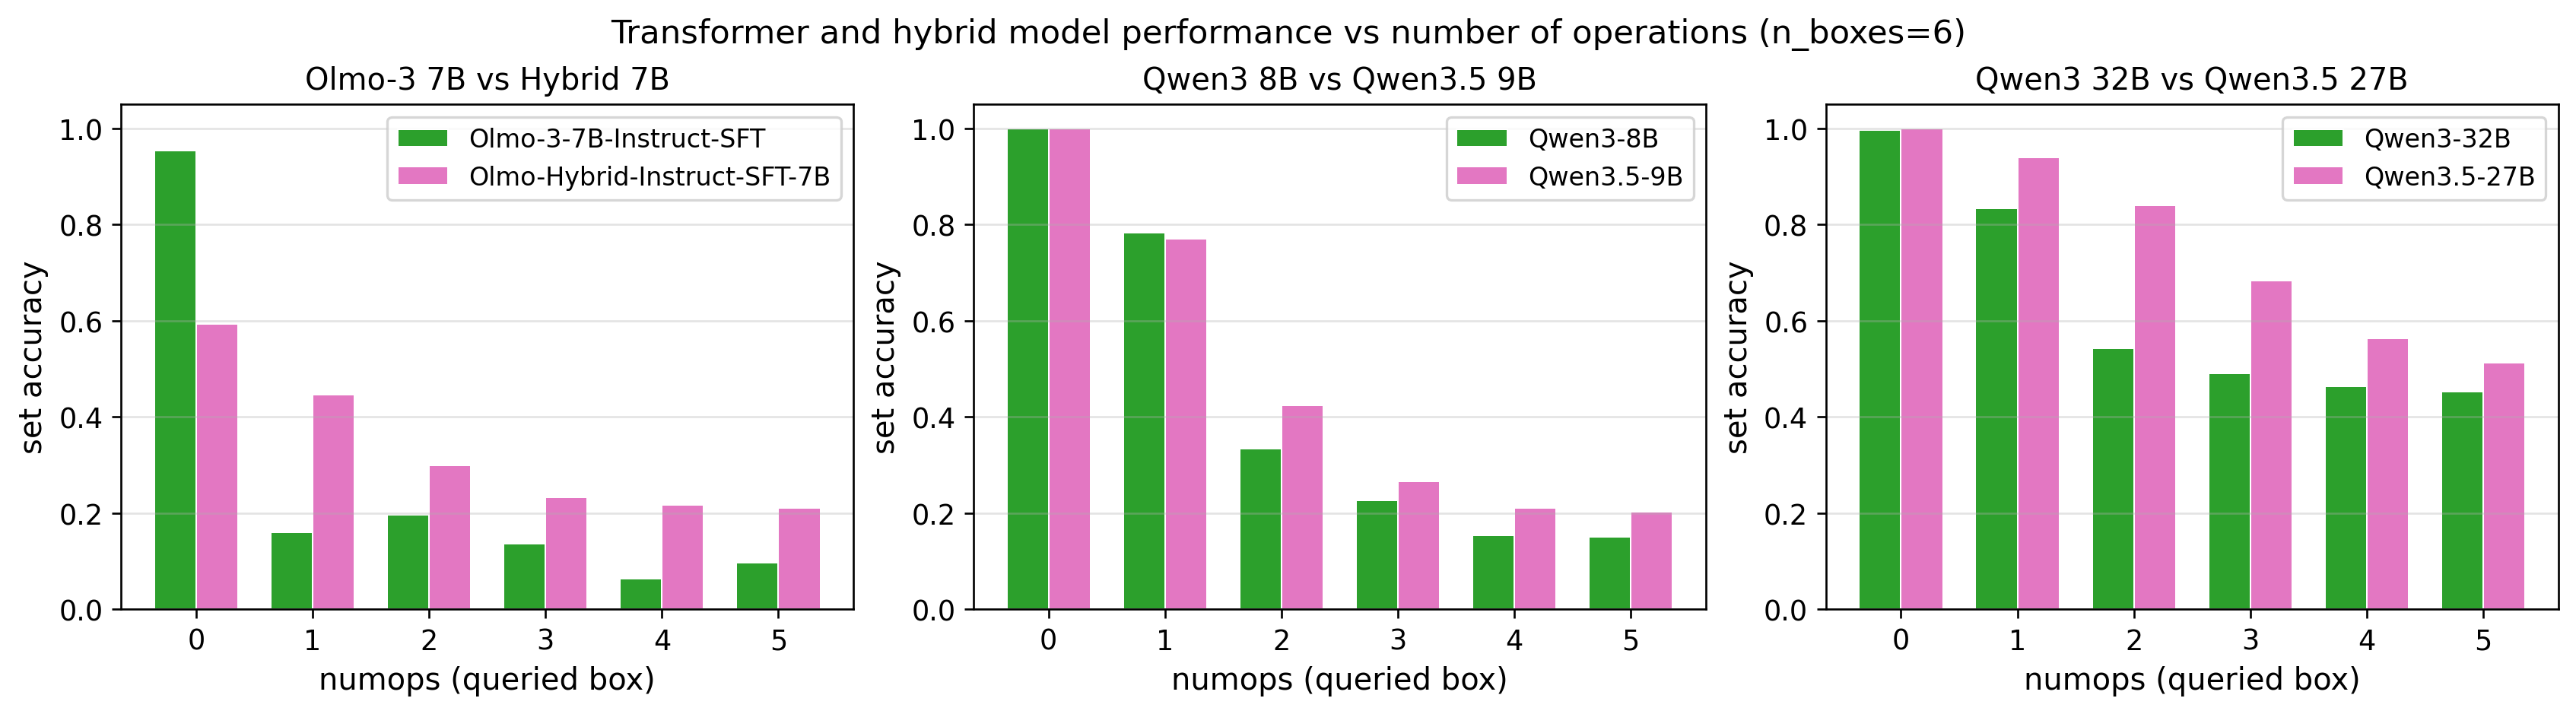
\includegraphics[width=1\linewidth]{assets//img/entity_tracking_nbox6_comparison.png}
    \caption{Comparison of entity-tracking task performance between pure-attention transformer models and similarly sized hybrid models. The x-axis indicates the number of operations (put, remove, or move) performed on the queried box, and the y-axis reports model prediction accuracy. Across model pairs, hybrid models tend to outperform their pure-attention counterparts as the number of operations increases, suggesting that hybrid architectures may be better suited for state-tracking tasks, especially in settings that require maintaining information over longer operation sequences.}
    \label{fig:entity_tracking_nbox6_comparison}
\end{figure}


\begin{figure}
    \centering
    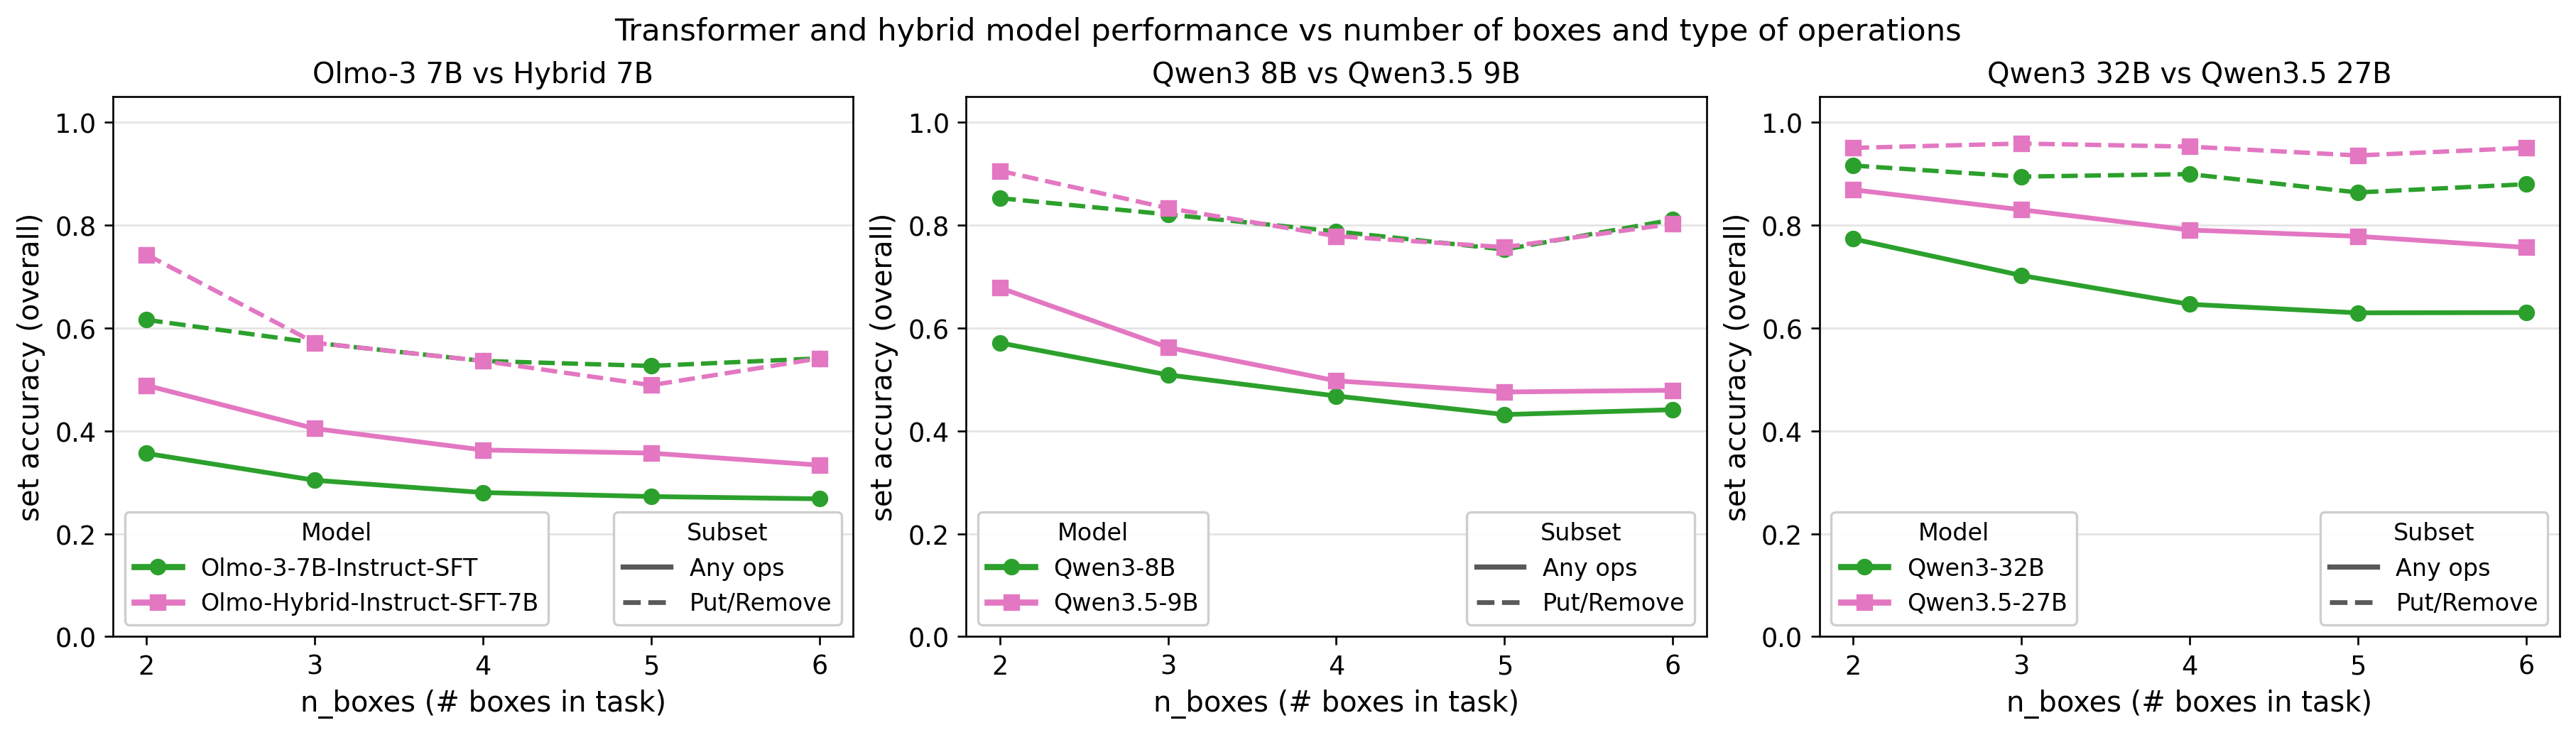
\includegraphics[width=1\linewidth]{assets//img/entity_tracking_nboxes_operations_comparison.png}
    \caption{Comparison of entity-tracking performance between pure-attention transformers and similarly sized hybrid models, across the number of boxes and operation types. Aggregated across number of operations, the performance gap between hybrid and pure-attention transformers persists across all box counts in our setting. This gap is wider when we include the move operation (move [object] from Box A to Box B), which simultaneously updates the state of two boxes, comparing to when we only consider the simpler put/remove operations, which again suggests a better state-tracking ability of the hybrid models.}
    \label{fig:entity_tracking_boxes_operations_comparison}
\end{figure}

\begin{figure*}[t]
    \centering
    % Row 1: Pure transformer Models (Top Row)
    \begin{subfigure}[b]{0.32\textwidth}
        \centering
        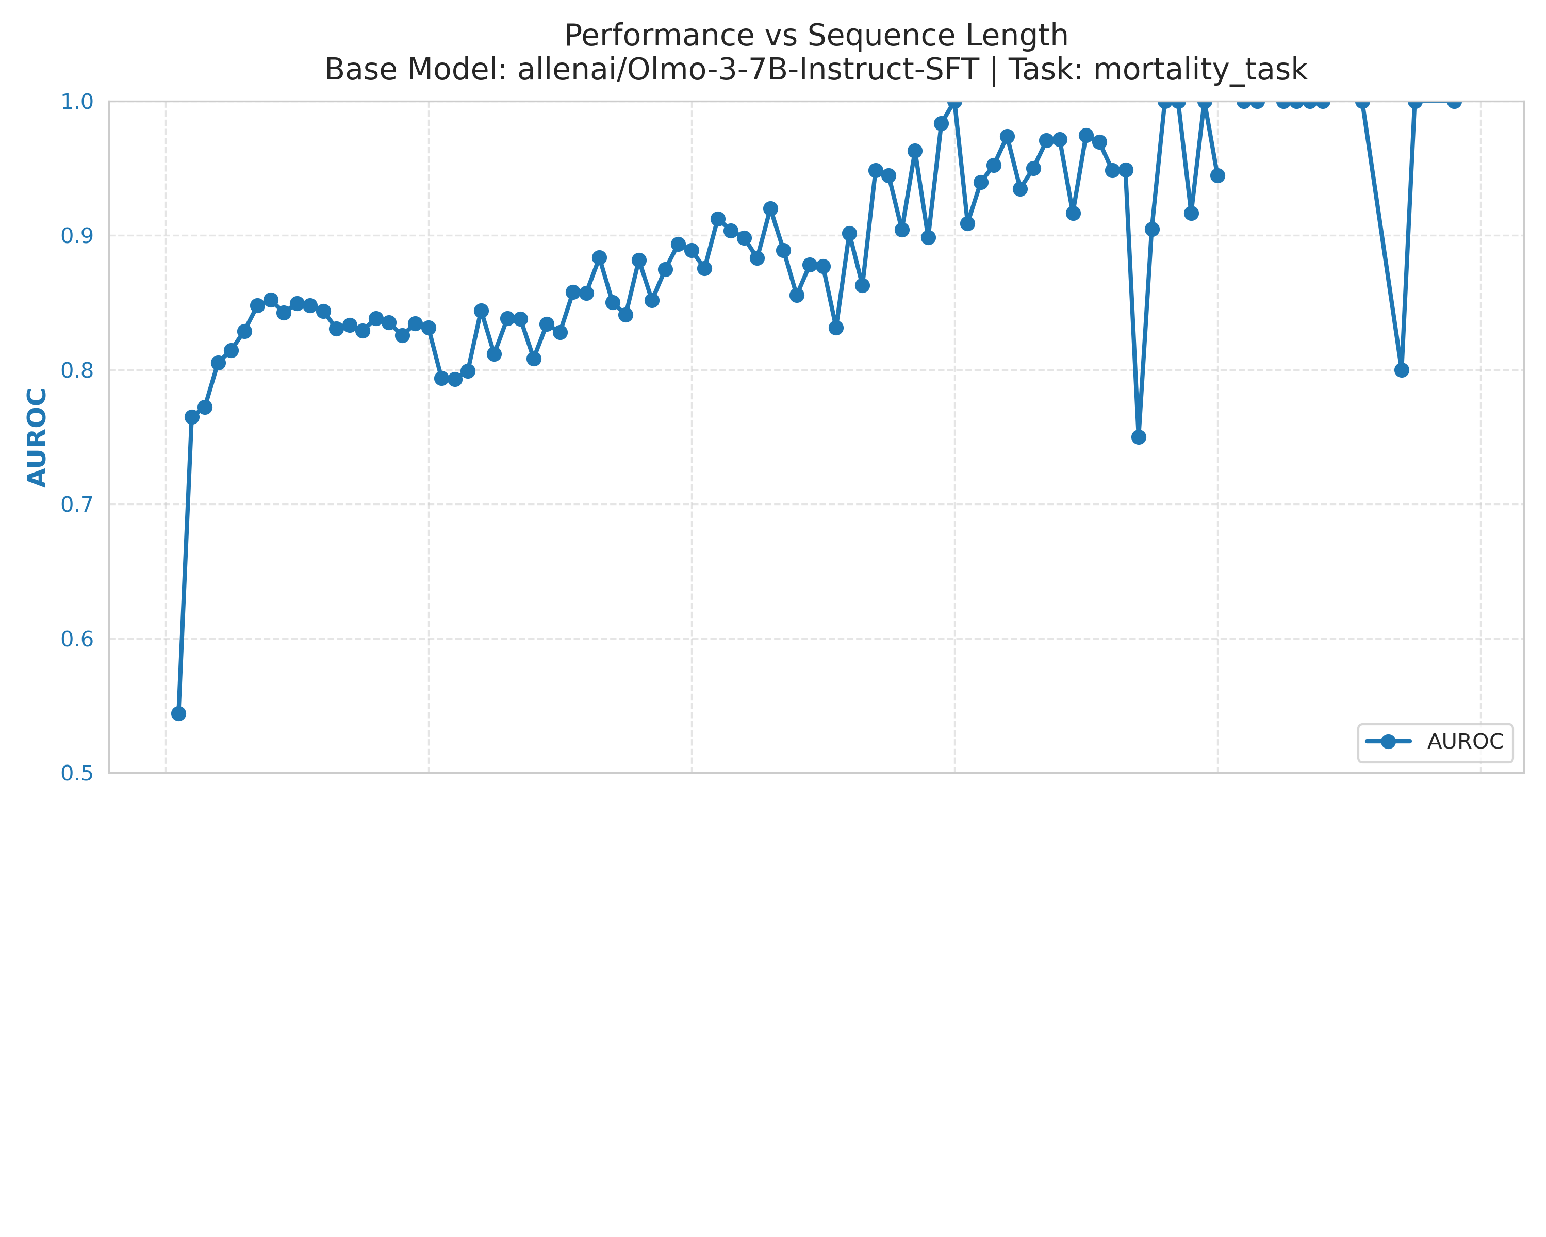
\includegraphics[width=\textwidth]{assets/img/allenai_Olmo-3-7B-Instruct-SFT_mortality_task_base_trajectory.pdf}
        \caption{OLMo-3-7B}
        \label{fig:seq_olmo_base}
    \end{subfigure}
    \hfill
    \begin{subfigure}[b]{0.32\textwidth}
        \centering
        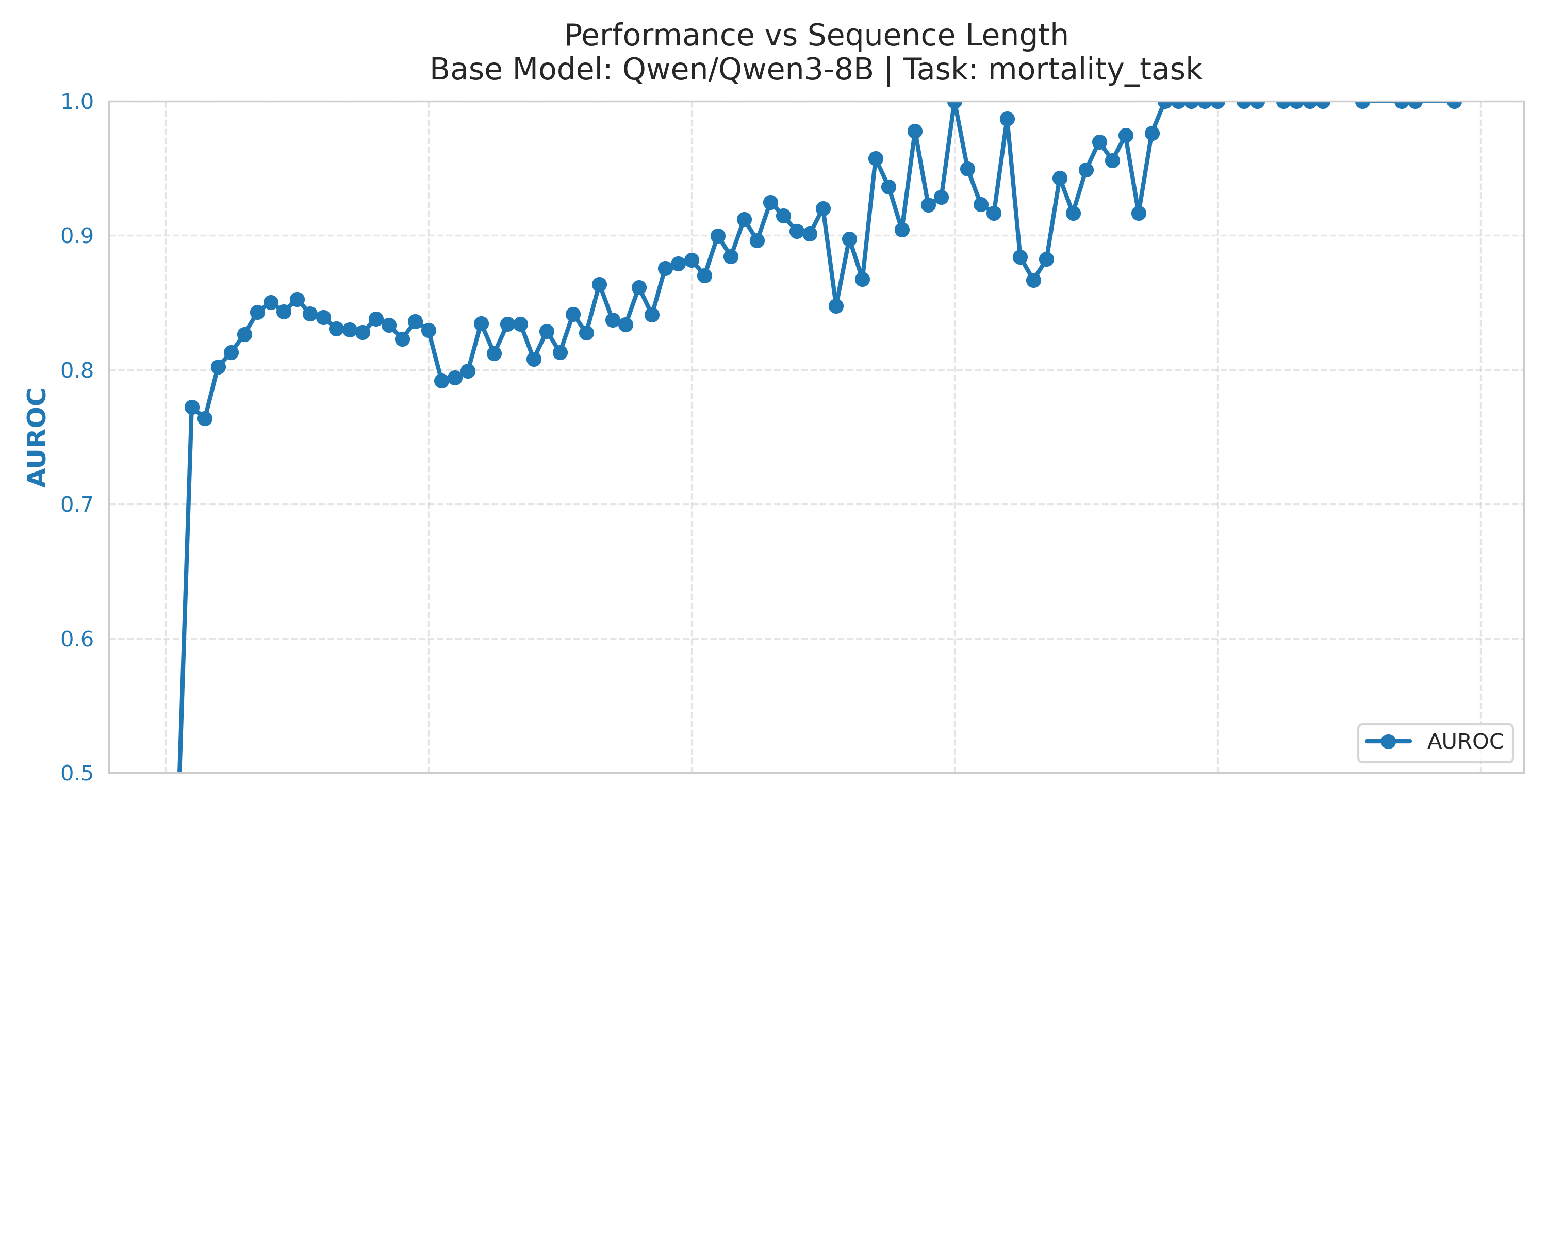
\includegraphics[width=\textwidth]{assets/img/Qwen_Qwen3-8B_mortality_task_base_trajectory.pdf}
        \caption{Qwen3-8B}
        \label{fig:seq_qwen_8b}
    \end{subfigure}
    \hfill
    \begin{subfigure}[b]{0.32\textwidth}
        \centering
        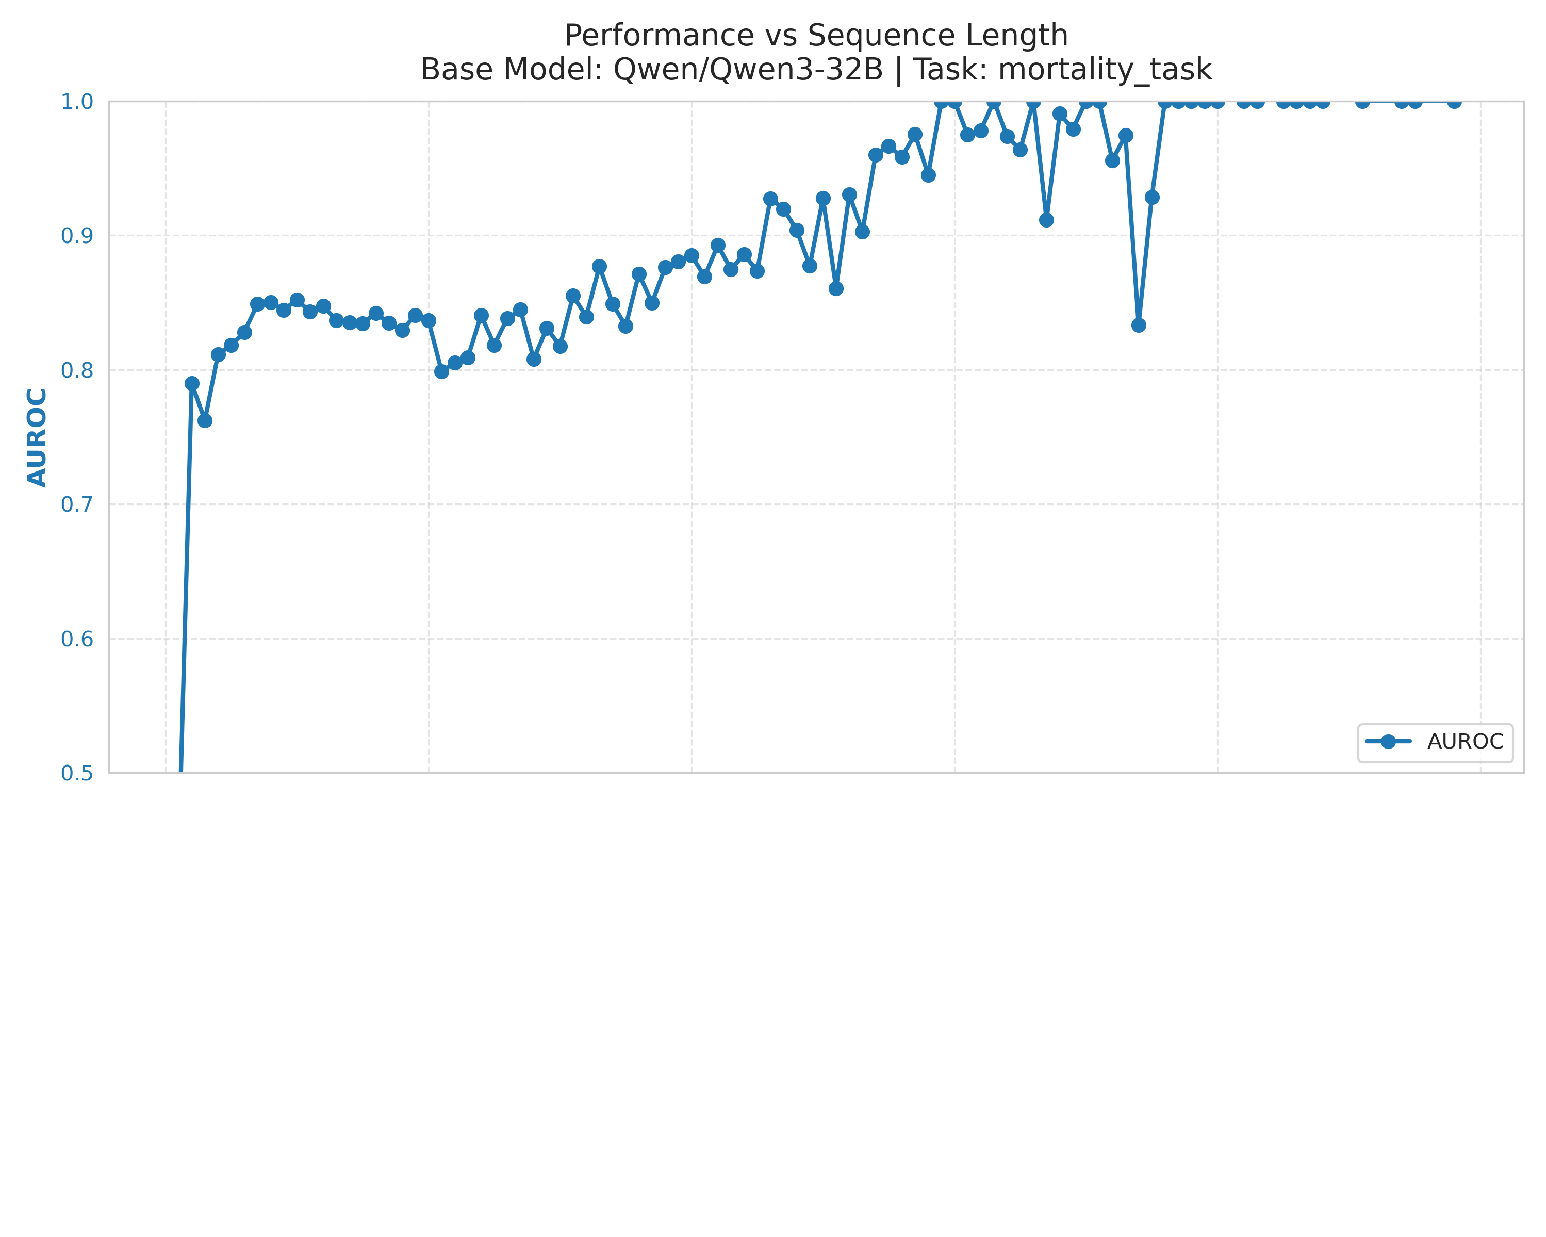
\includegraphics[width=\textwidth]{assets/img/Qwen_Qwen3-32B_mortality_task_base_trajectory.pdf}
        \caption{Qwen3-32B}
        \label{fig:seq_qwen_32b}
    \end{subfigure}
    
    \vspace{0.5em} % Reduced vertical space between rows
    
    % Row 2: Hybrid Models (Middle Row)
    \begin{subfigure}[b]{0.32\textwidth}
        \centering
        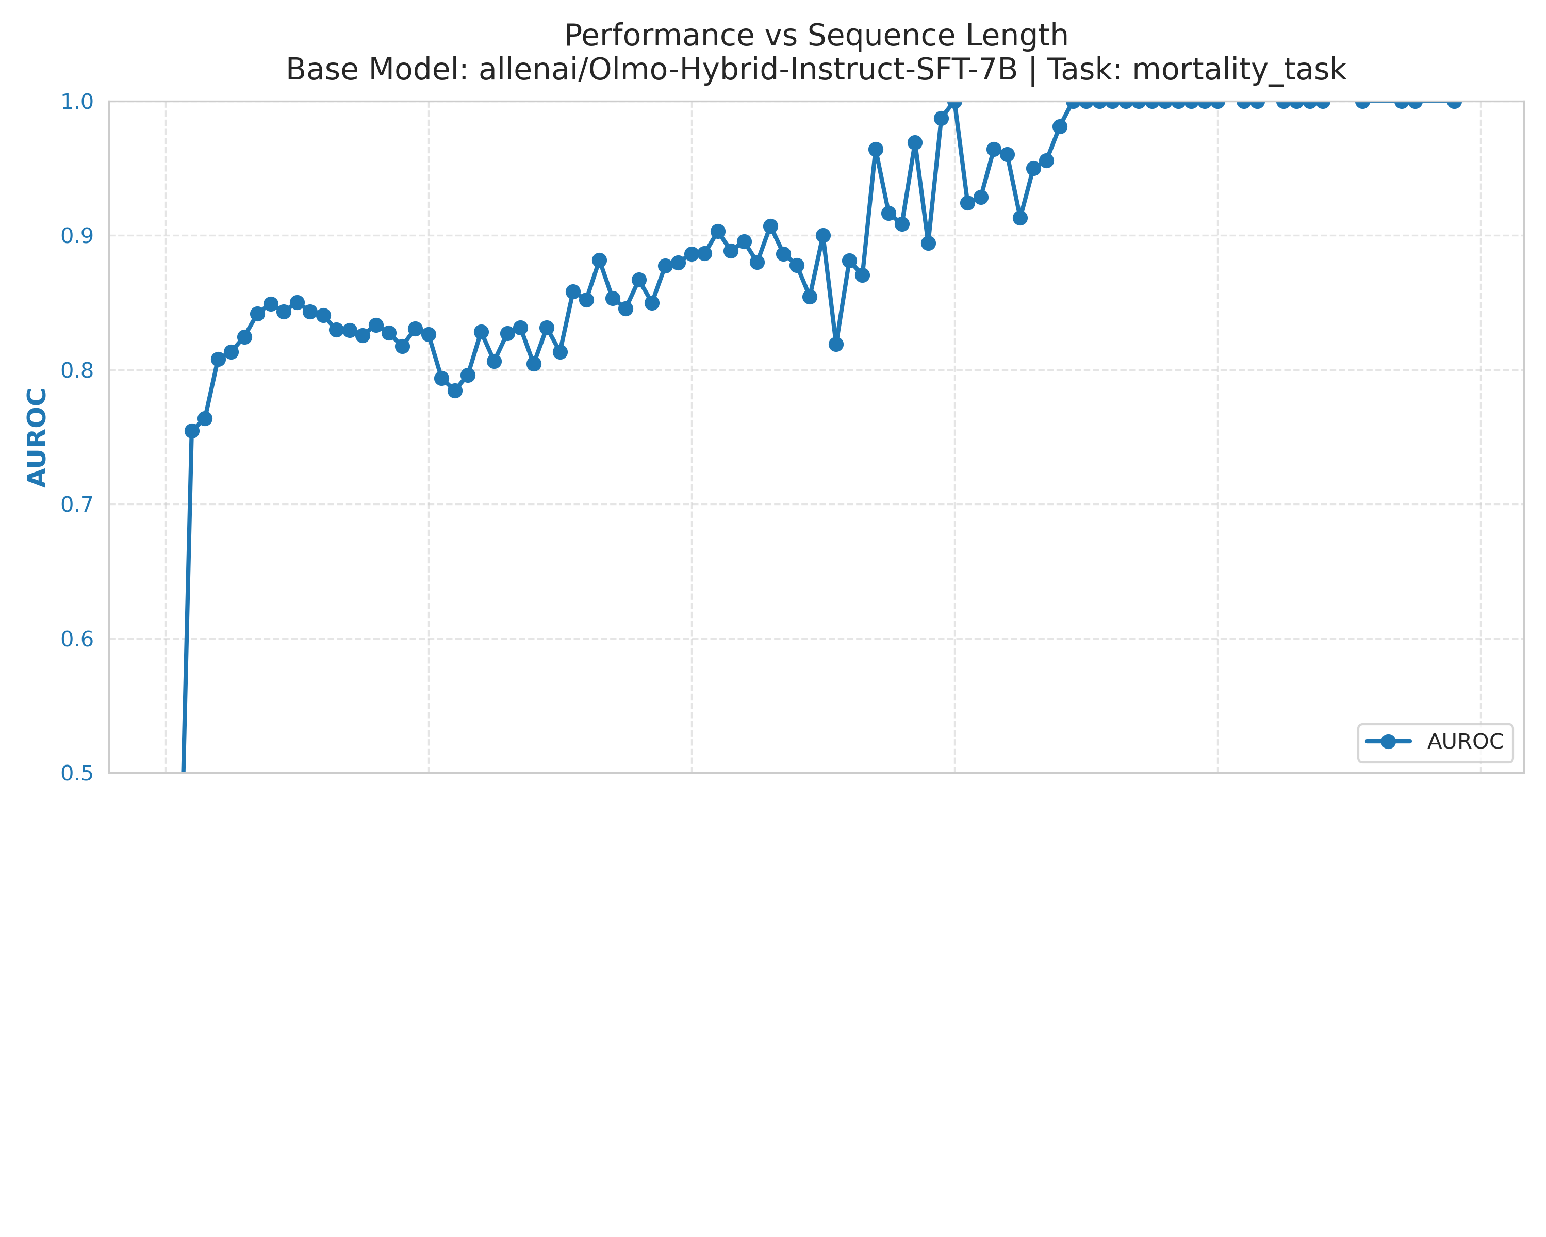
\includegraphics[width=\textwidth]{assets/img/allenai_Olmo-Hybrid-Instruct-SFT-7B_mortality_task_base_trajectory.pdf}
        \caption{OLMo-Hybrid-7B}
        \label{fig:seq_olmo_hybrid}
    \end{subfigure}
    \hfill
    \begin{subfigure}[b]{0.32\textwidth}
        \centering
        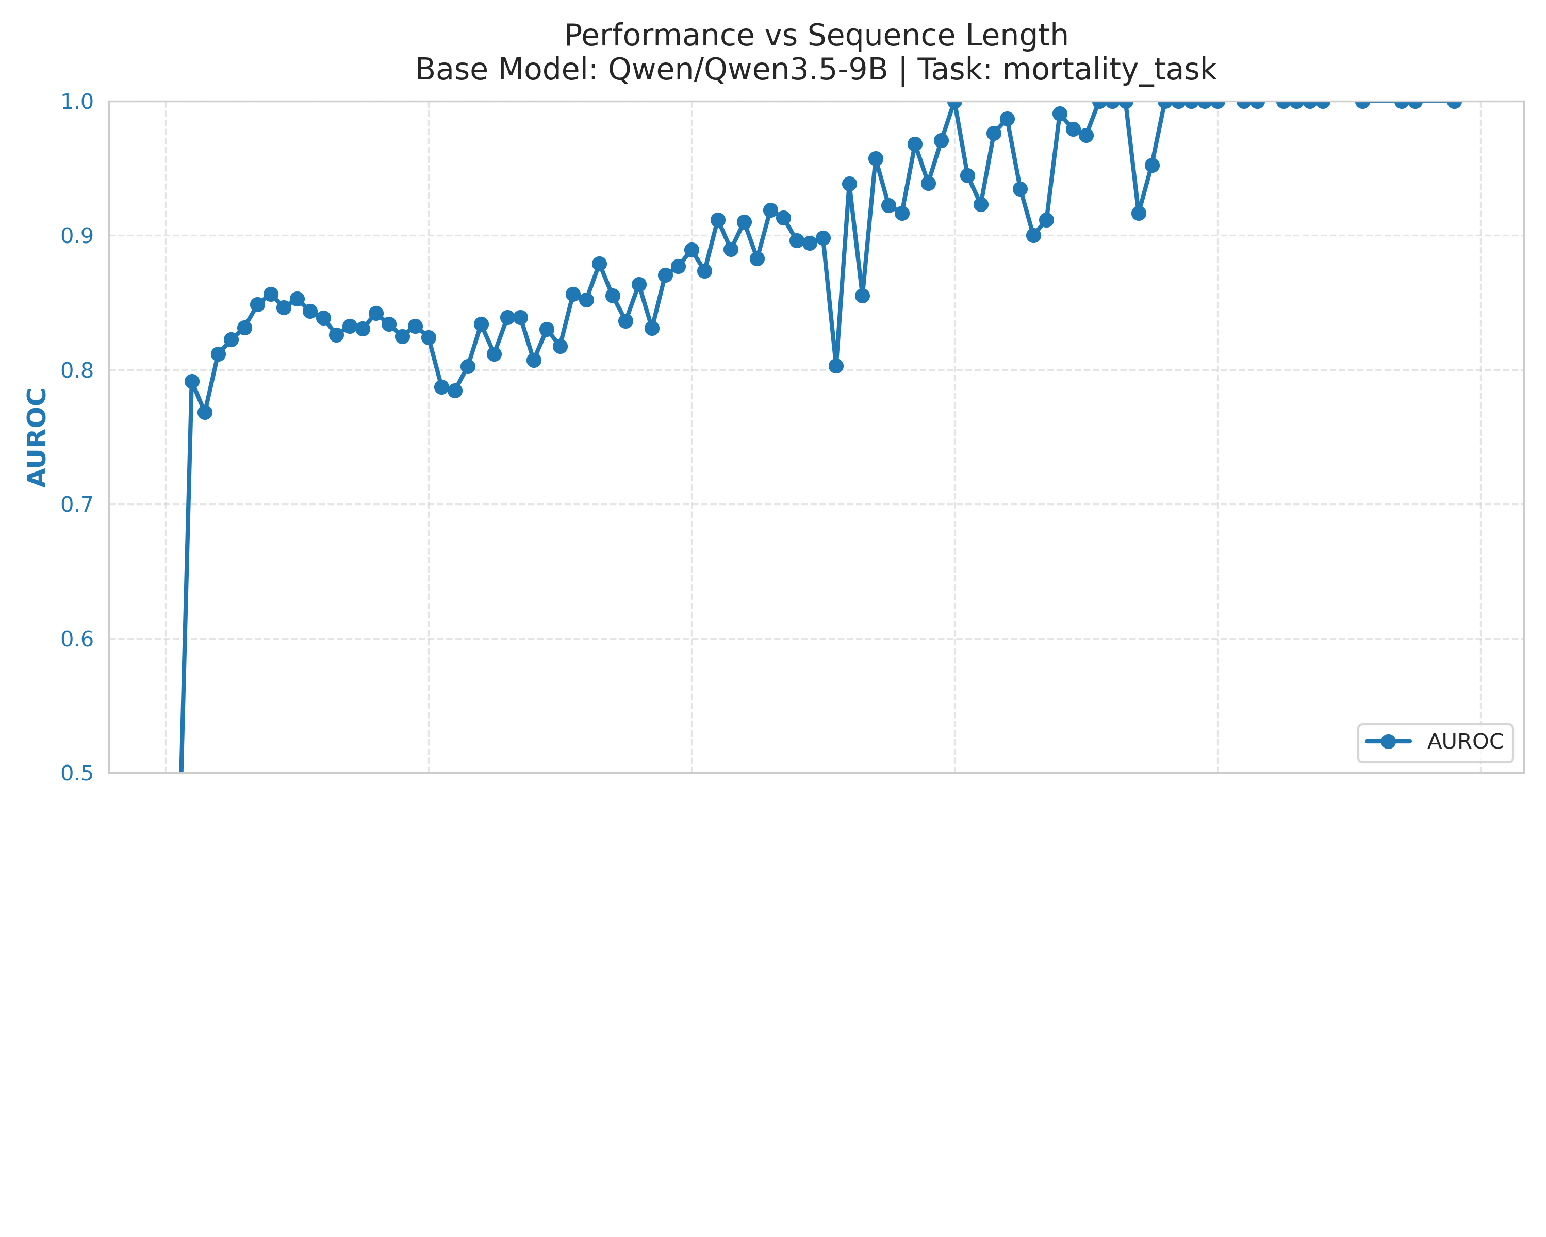
\includegraphics[width=\textwidth]{assets/img/Qwen_Qwen3.5-9B_mortality_task_base_trajectory.pdf}
        \caption{Qwen3.5-9B}
        \label{fig:seq_qwen_9b}
    \end{subfigure}
    \hfill
    \begin{subfigure}[b]{0.32\textwidth}
        \centering
        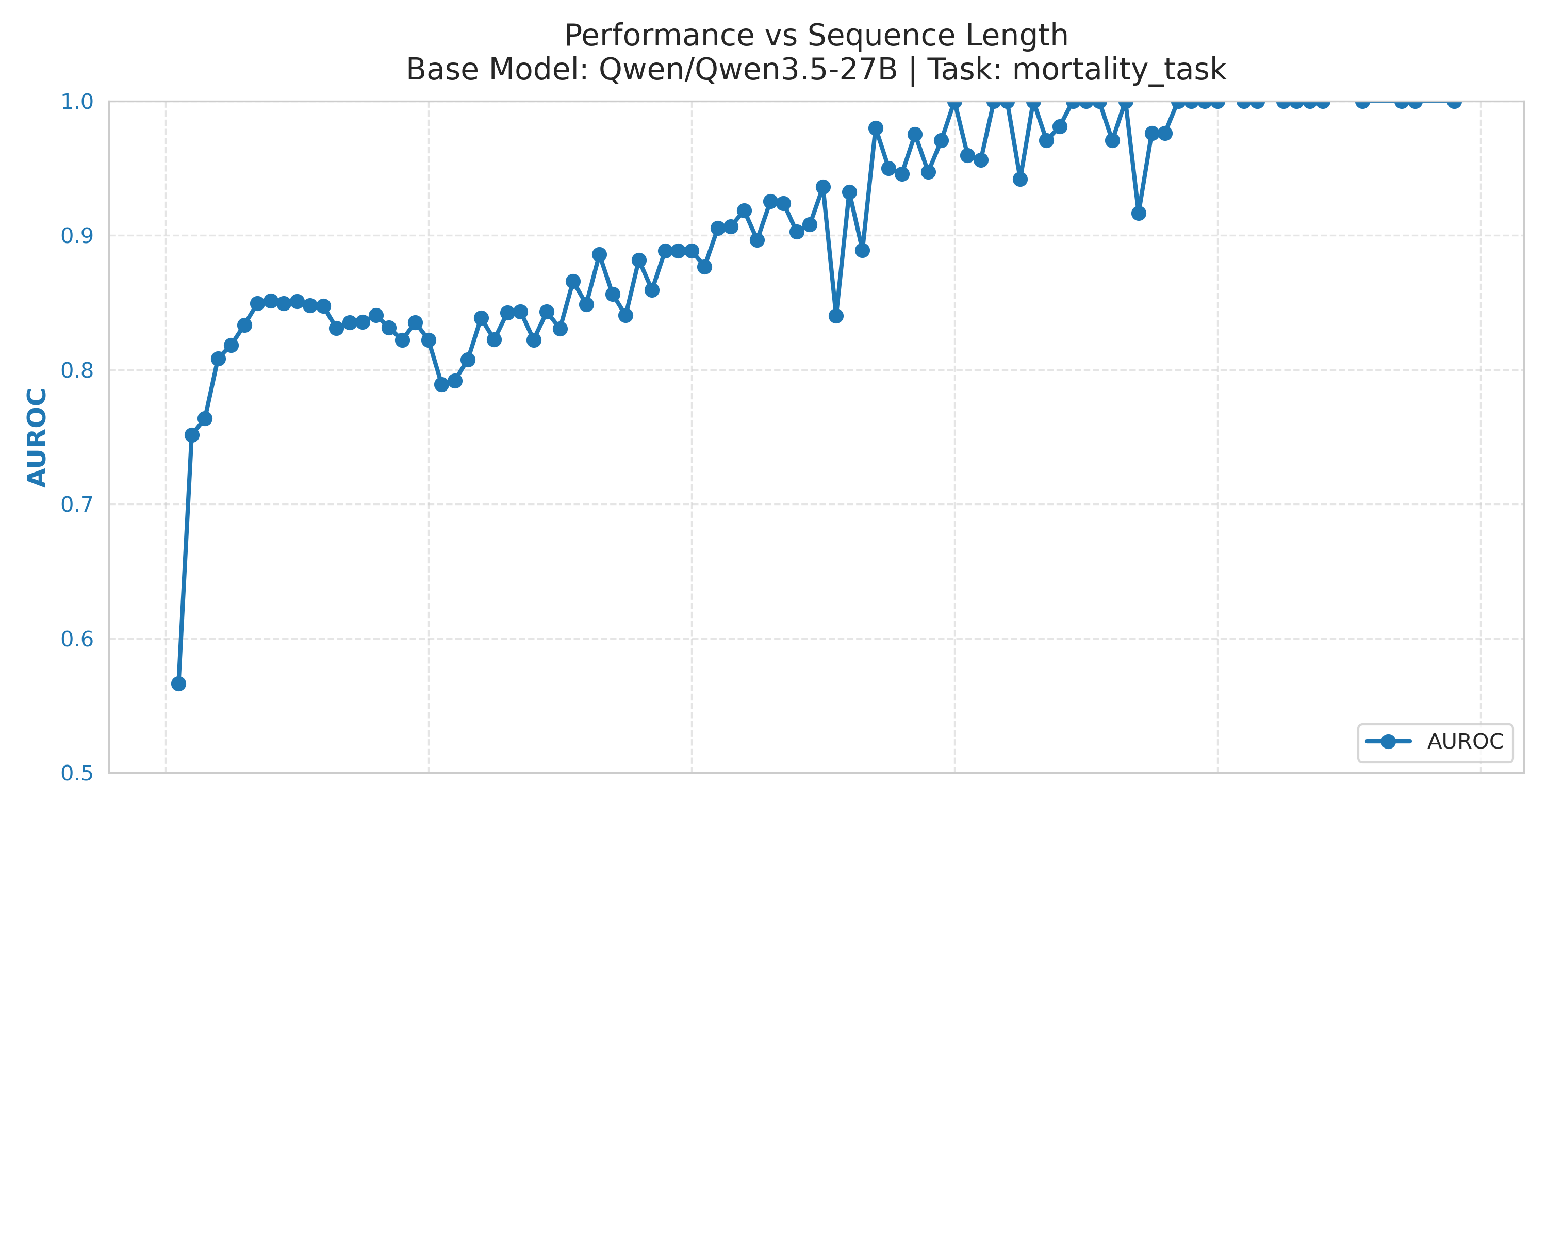
\includegraphics[width=\textwidth]{assets/img/Qwen_Qwen3.5-27B_mortality_task_base_trajectory.pdf}
        \caption{Qwen3.5-27B}
        \label{fig:seq_qwen_27b}
    \end{subfigure}

    \vspace{0.5em} % Reduced vertical space between rows

    % Row 3: Event Distributions (Bottom Row)
    \begin{subfigure}[b]{0.32\textwidth}
        \centering
        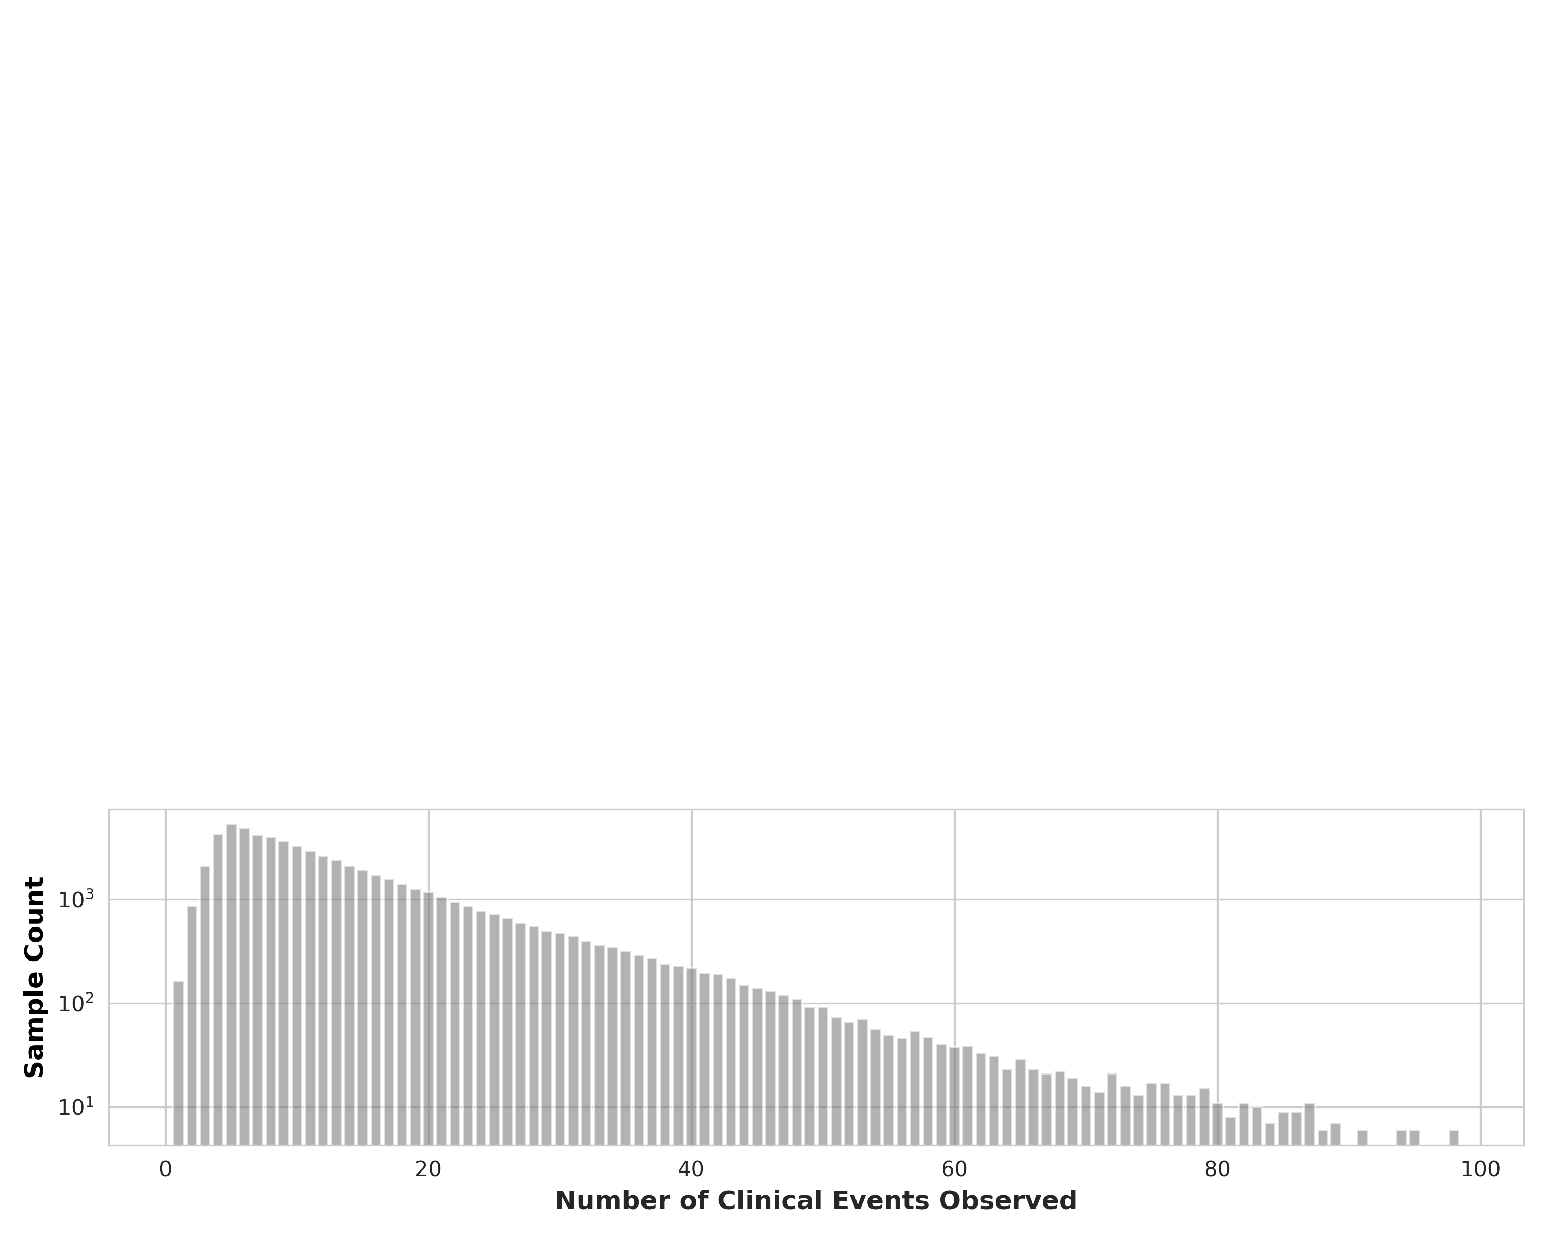
\includegraphics[width=\textwidth]{assets/img/events.pdf}
        \label{fig:seq_events_1}
    \end{subfigure}
    \hfill
    \begin{subfigure}[b]{0.32\textwidth}
        \centering
        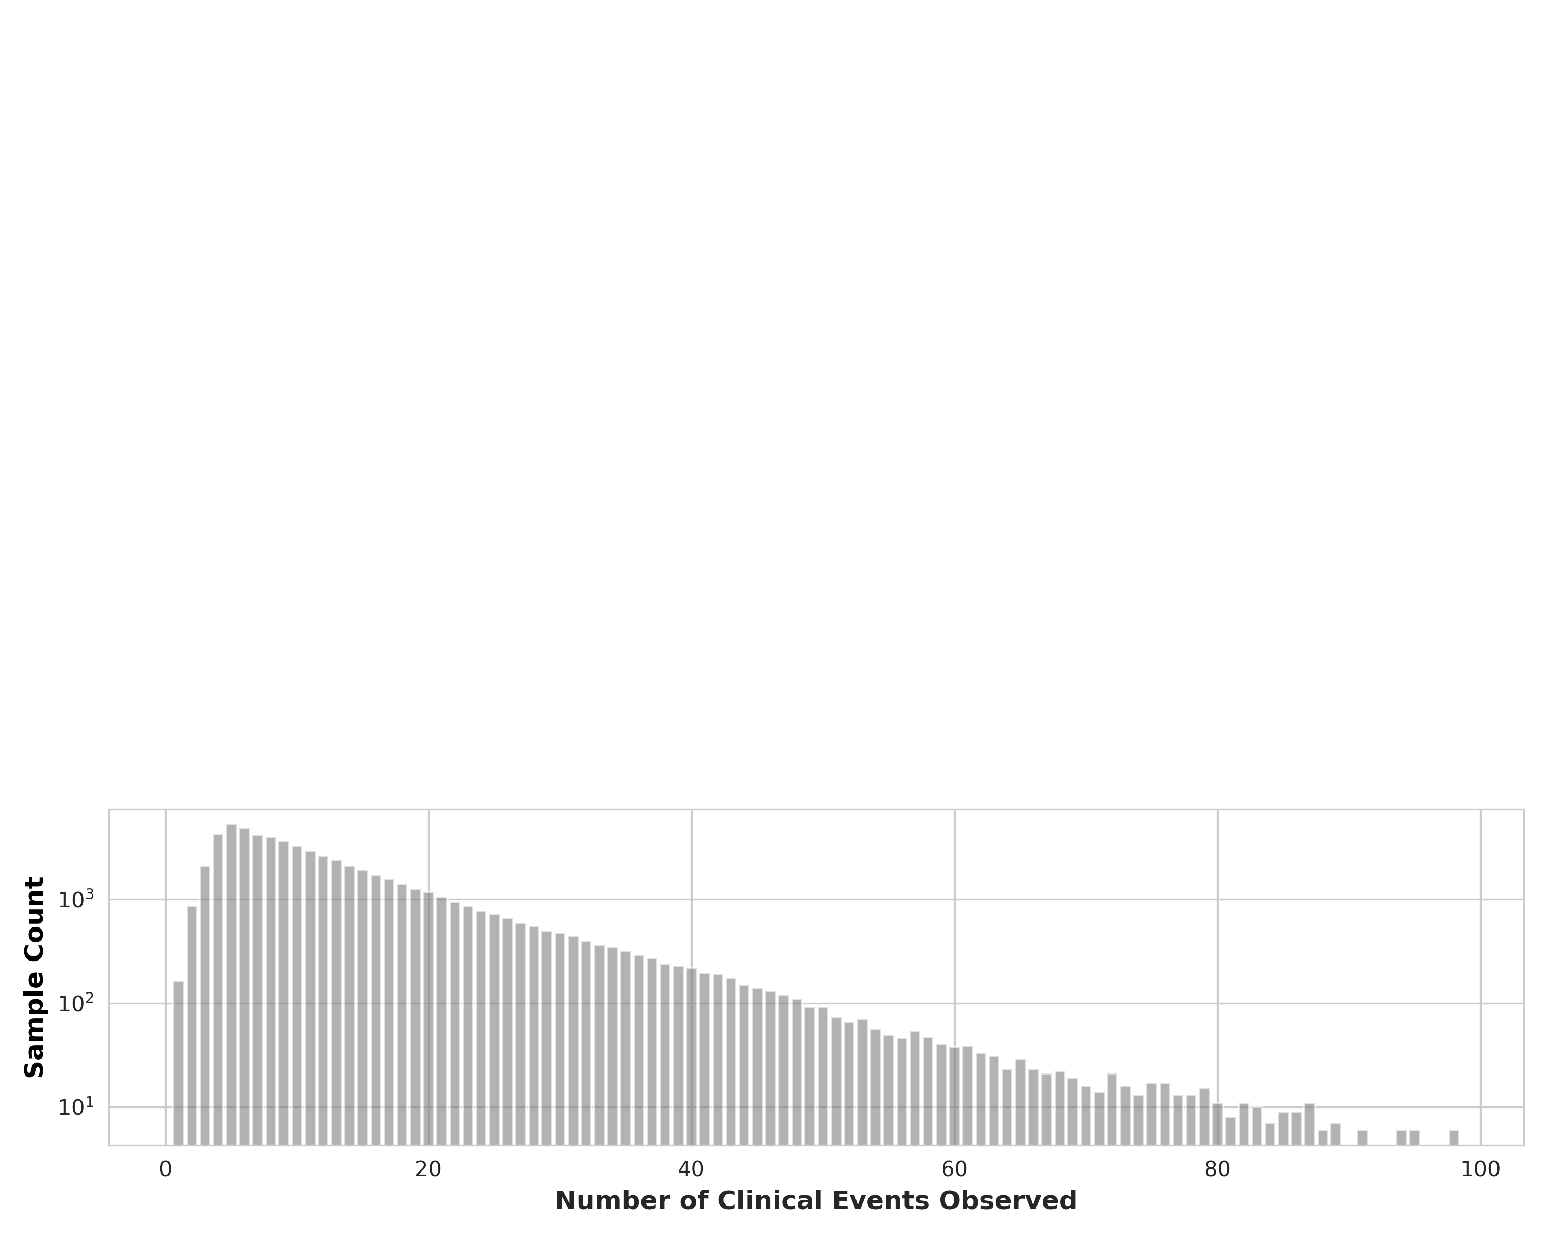
\includegraphics[width=\textwidth]{assets/img/events.pdf}
        \label{fig:seq_events_2}
    \end{subfigure}
    \hfill
    \begin{subfigure}[b]{0.32\textwidth}
        \centering
        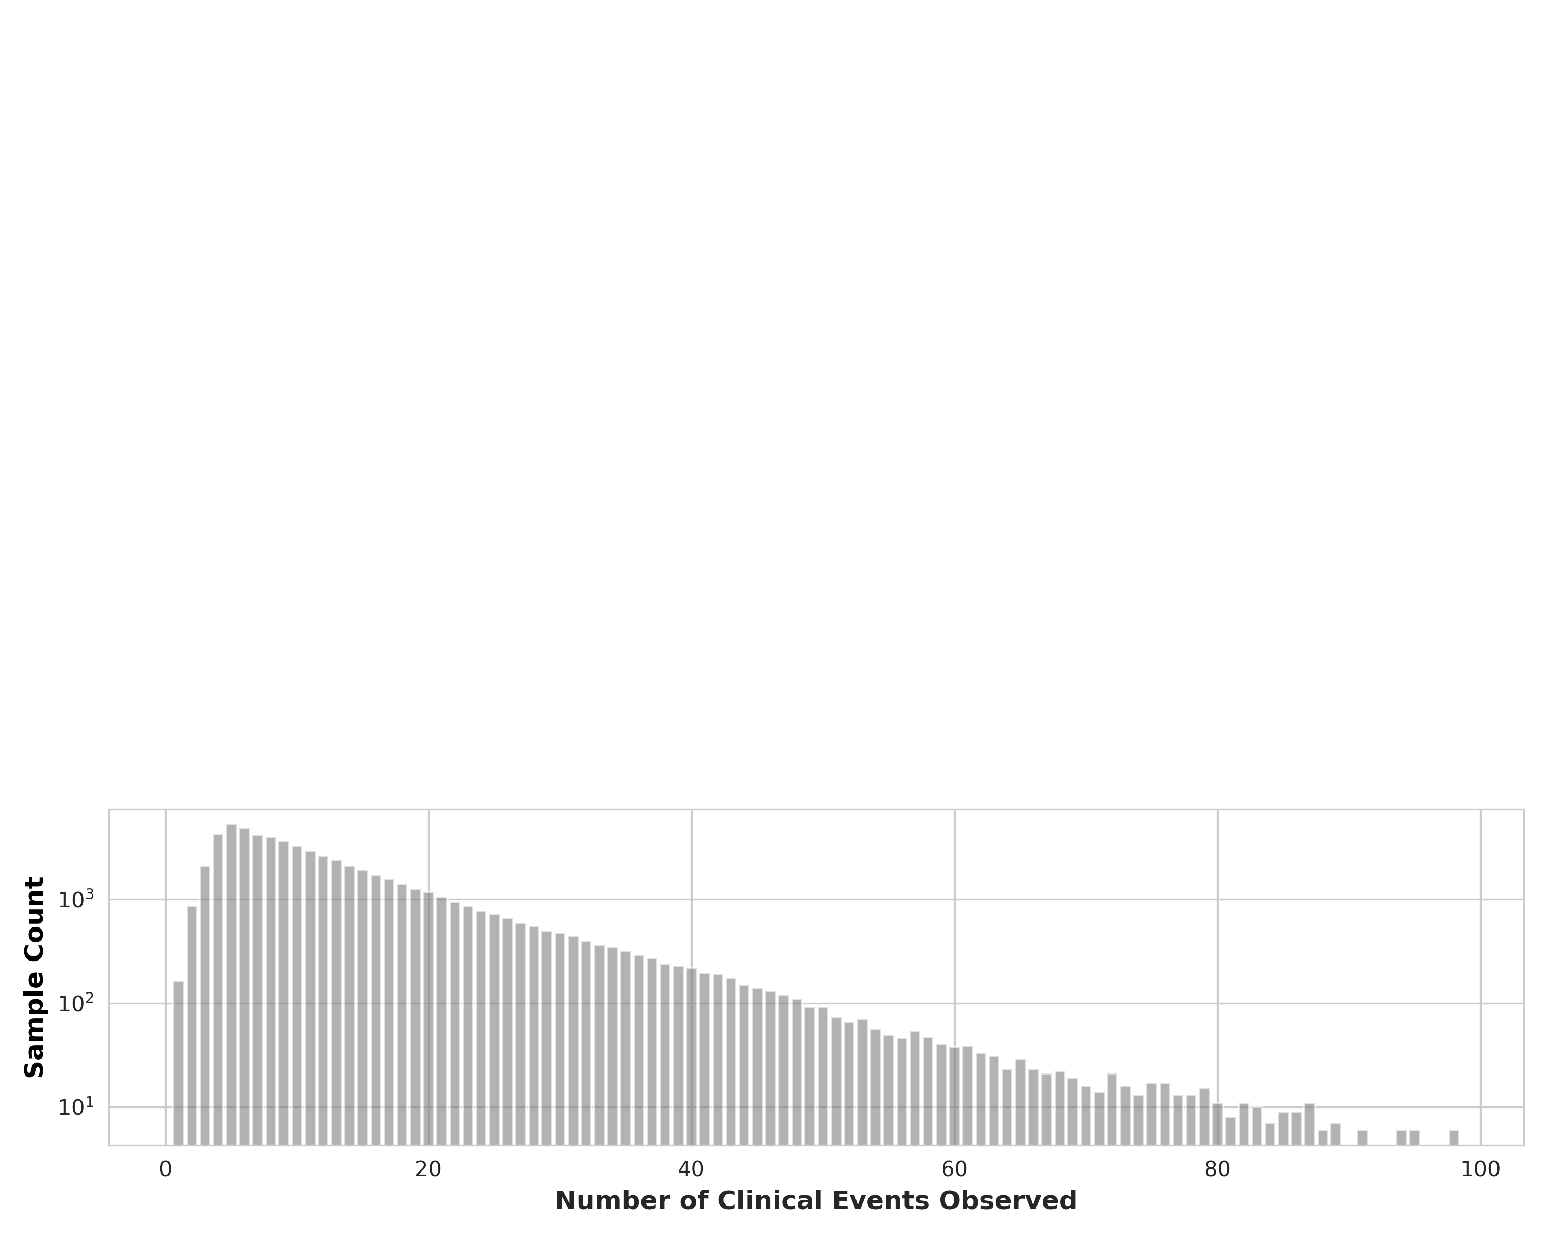
\includegraphics[width=\textwidth]{assets/img/events.pdf}
        \label{fig:seq_events_3}
    \end{subfigure}
    
    \caption{Comparison of task performance between pure-attention transformer models (top row), hybrid models (middle row), and corresponding distribution of the number of events (bottom row). The x-axis indicates the number of clinical events, and the y-axis reports model prediction AUROC. We broadly observe similar performance trends across both sets of models, model sizes, and number of events, with strong performance on stays with a higher number of clinical events. This broadly suggests that both attention-only and hybrid language model decoders are well-suited to model patient stay trajectories across varying stay lengths.}
    \label{fig:clinical-seq_performance}
\end{figure*}

\subsubsection{Layer-wise Ablation Results}


\begin{figure}[t]
    \centering

    \begin{subfigure}[t]{0.49\linewidth}
        \centering
        \includegraphics[width=\linewidth]{assets/img/olmo_layerwise_ablation_comparison.png}
        \caption{OLMo 7B versus OLMo Hybrid.}
        \label{fig:olmo_layerwise_ablation_comparison}
    \end{subfigure}
    \hfill
    \begin{subfigure}[t]{0.49\linewidth}
        \centering
        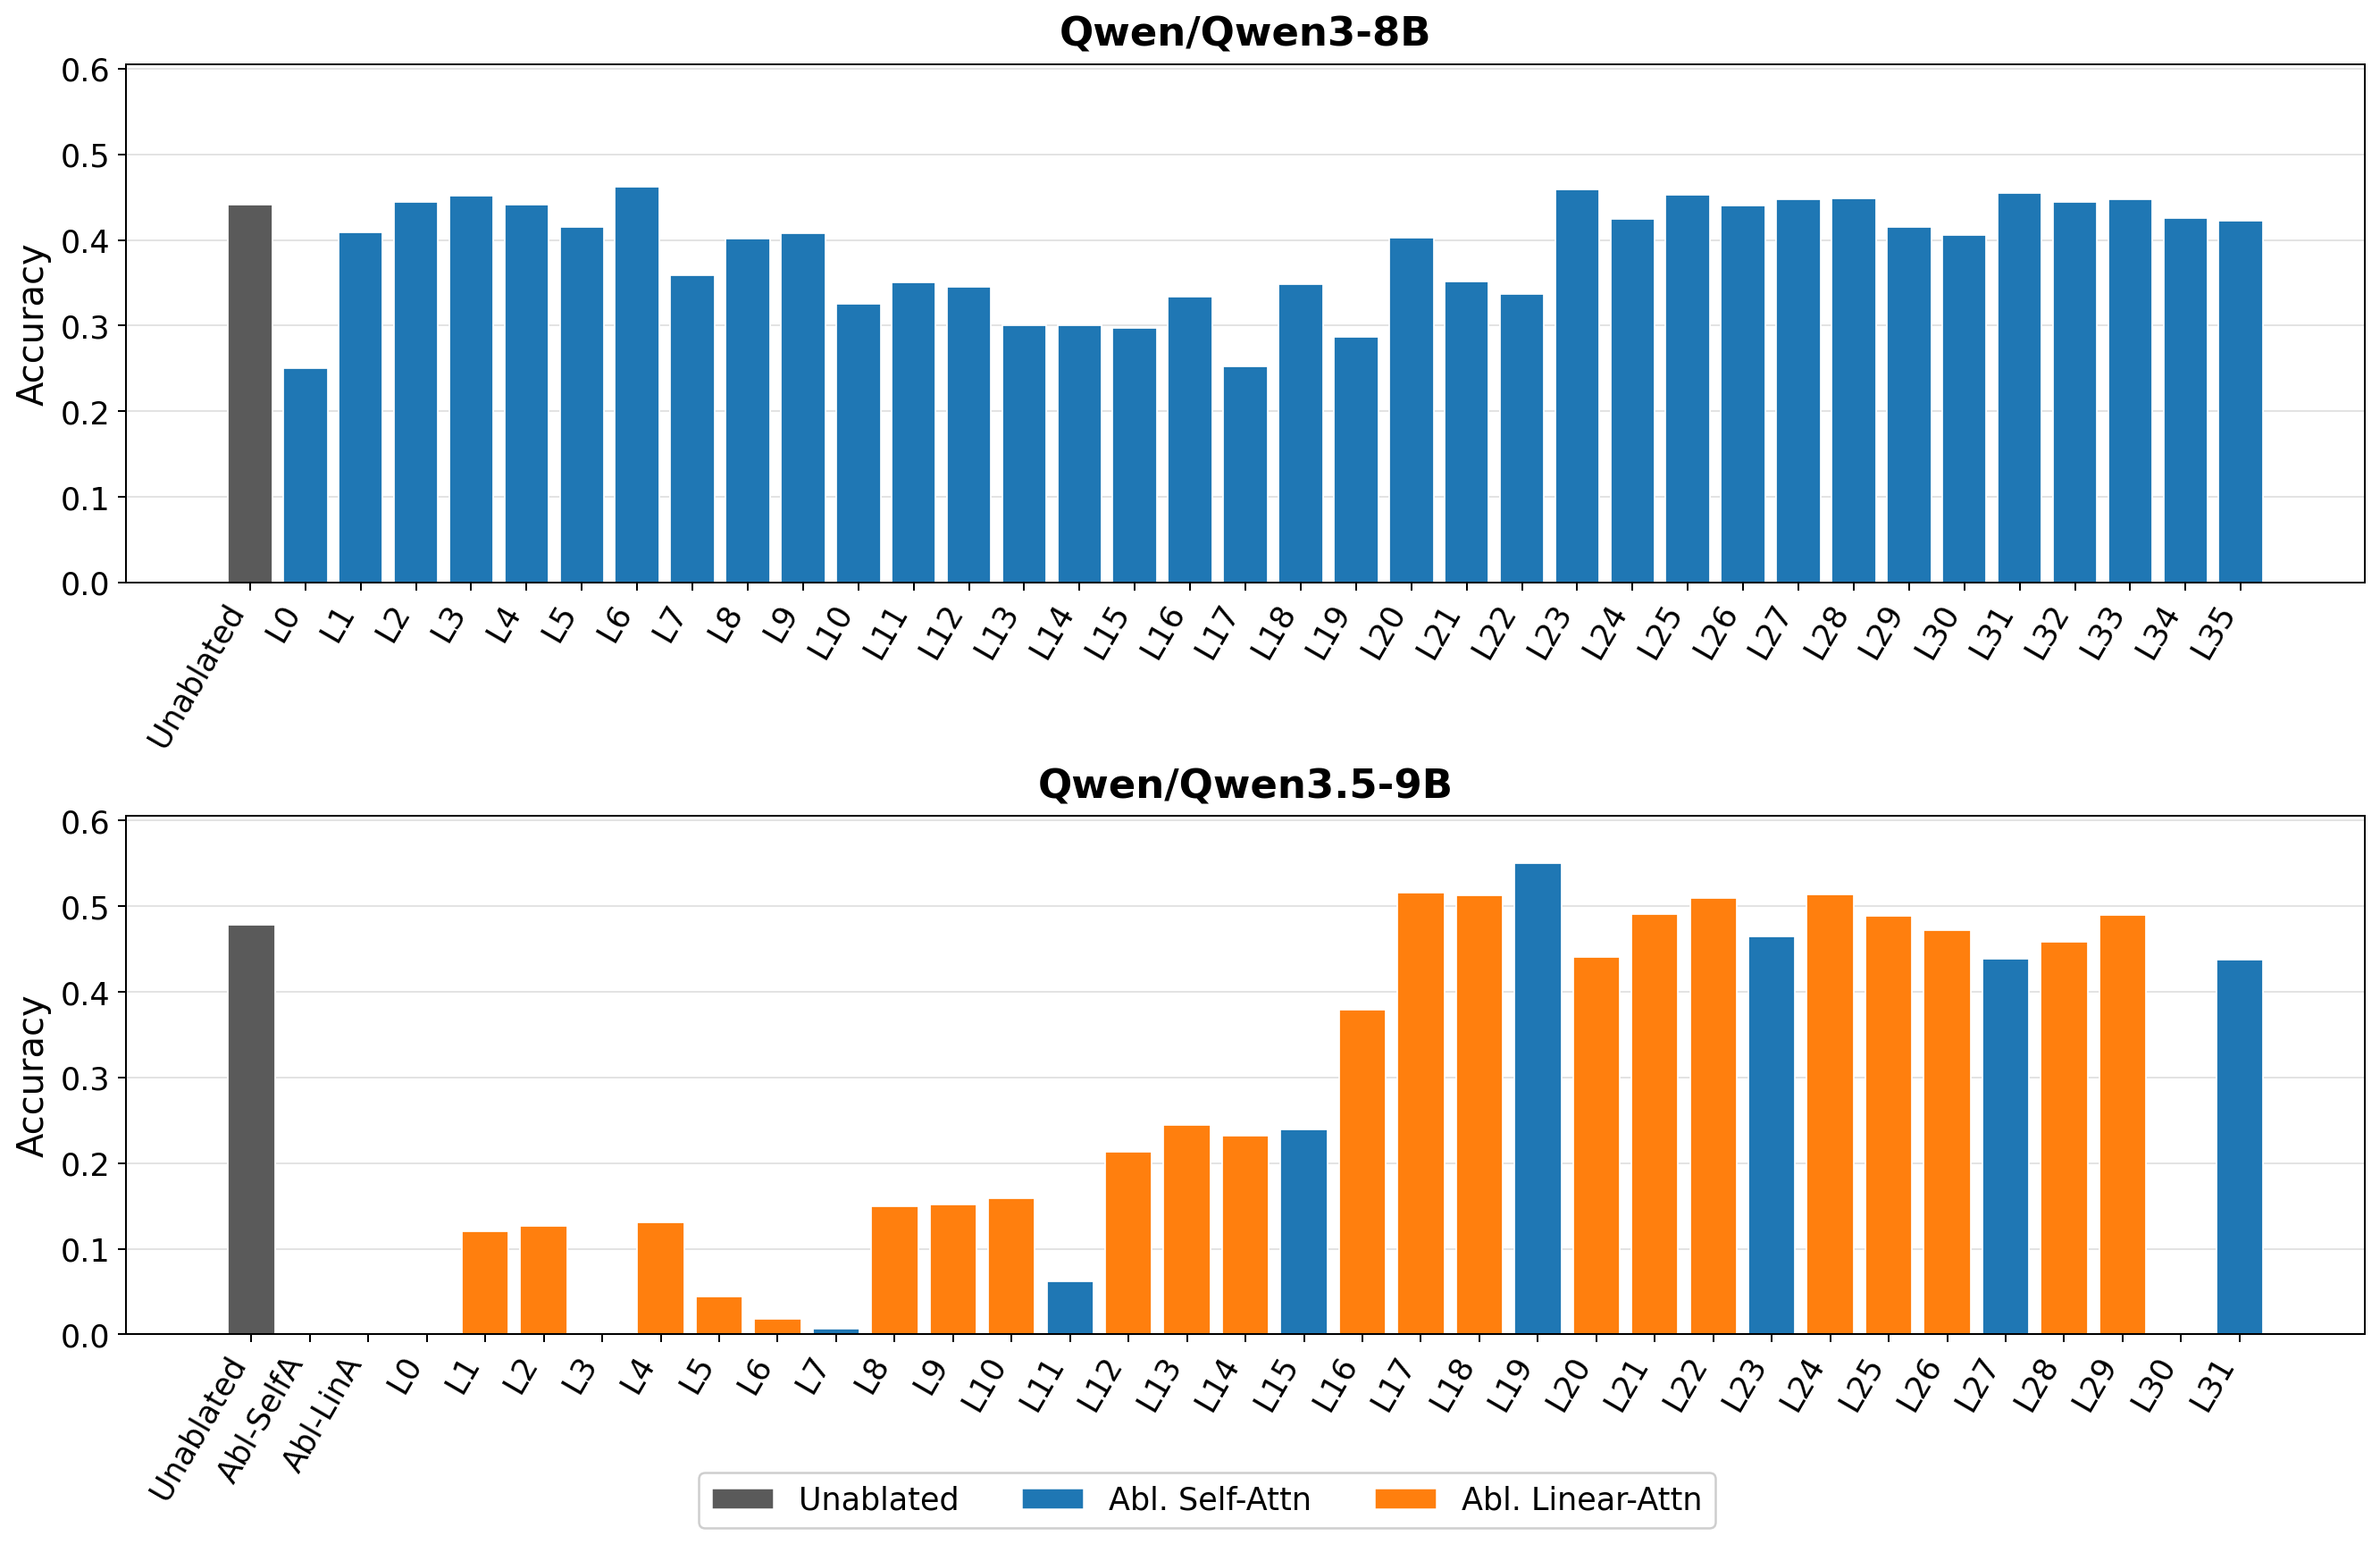
\includegraphics[width=\linewidth]{assets/img/qwen_small_layerwise_ablation_comparison.png}
        \caption{Qwen3-8B versus Qwen3.5-9B.}
        \label{fig:qwen_small_layerwise_ablation_comparison}
    \end{subfigure}

    \caption{Layer-wise ablation results for OLMo and Qwen models. Each bar shows entity-tracking accuracy after ablating 1 attention layer or a group of attention layers (for the hybrid models), with gray indicating the unablated baseline, blue indicating self-attention ablations, and orange indicating linear-attention ablations in hybrid models.}
    \label{fig:layerwise_ablation_comparison}
\end{figure}

% \begin{figure}
%     \centering
%     \includegraphics[width=1\linewidth]{assets//img/olmo_layerwise_ablation_comparison.png}
%     \caption{Enter Caption}    \label{fig:olmo_layerwise_ablation_comparison}
% \end{figure}


% \begin{figure}
%     \centering
%     \includegraphics[width=1\linewidth]{assets//img/qwen_small_comparison_layerwise_ablation.png}
%     \caption{Enter Caption} \label{fig:qwen_small_comparison_layerwise_ablation}
% \end{figure}

\paragraph{Entity Tracking} Figure~\ref{fig:layerwise_ablation_comparison} shows that ablating individual attention layers has different effects across pure-attention and hybrid architectures. In the pure-attention models, performance is relatively robust to ablating most single layers, suggesting redundancy across self-attention modules. In contrast, the hybrid models show stronger layer-specific sensitivity, especially in earlier layers. For OLMo-Hybrid, ablating early linear-attention layers leads to particularly large performance drops, while for Qwen3.5-9B, ablating early self-attention layers leads to huge performance drops to an accuracy of near zero. These mixed patterns suggest that hybrid models do not rely on a single attention type in a cleanly separable way; rather, self-attention and linear-attention modules appear to interact in supporting state tracking.

\subsubsection{Entity-Tracking: Activation Patching Results}

\section{Conclusion}


\bibliographystyle{unsrtnat}  
\bibliography{bib}  
\medskip
{
\small


\clearpage
%%%%%%%%%%%%%%%%%%%%%%%%%%%%%%%%%%%%%%%%%%%%%%%%%%%%%%%%%%%%
\appendix
\renewcommand{\thefigure}{A.\arabic{figure}}
\setcounter{figure}{0}

\renewcommand{\thetable}{A.\arabic{table}}
\setcounter{table}{0}

\section{Implementation Details}

\subsection{Models Tested}
We evaluate six models drawn from two model families: OLMo and Qwen. Within each family, we compare pure-transformer models against hybrid models that combine standard full-attention layers with linear-attention modules.

\begin{center}
\begin{tabular}{lll}
\toprule
\textbf{Label} & \textbf{Architecture} & \textbf{HuggingFace ID} \\
\midrule
OLMo-3 7B      & Pure transformer (SFT) & \texttt{allenai/Olmo-3-7B-Instruct-SFT} \\
OLMo-Hybrid 7B & Hybrid (SFT) & \texttt{allenai/Olmo-Hybrid-Instruct-SFT-7B} \\
Qwen3 8B       & Pure transformer & \texttt{Qwen/Qwen3-8B} \\
Qwen3 32B      & Pure transformer & \texttt{Qwen/Qwen3-32B} \\
Qwen3.5 9B     & Hybrid & \texttt{Qwen/Qwen3.5-9B} \\
Qwen3.5 27B    & Hybrid & \texttt{Qwen/Qwen3.5-27B} \\
\bottomrule
\end{tabular}
\end{center}

The OLMo-Hybrid and Qwen3.5 models interleave standard full-attention layers with linear-attention modules, including GatedDeltaNet-style layers. This makes them natural candidates for studying whether hybrid architectures differ from pure transformers on in-context retrieval and state-tracking tasks.

For the hybrid models, full-attention and linear-attention layers follow a regular interleaving pattern. 
In the 32-layer configuration, standard self-attention layers appear at layers 3, 7, 11, 15, 19, 23, 27, and 31, while the remaining layers use linear-attention modules: layers 0--2, 4--6, 8--10, 12--14, 16--18, 20--22, 24--26, and 28--30. 
For deeper 35-layer variants, the same hybrid pattern is extended to the additional layers, with standard full-attention layers inserted periodically among linear-attention modules.

\section{In-Content Retrieval: Colored Objects Task}

\begin{figure}[t]
    \centering
    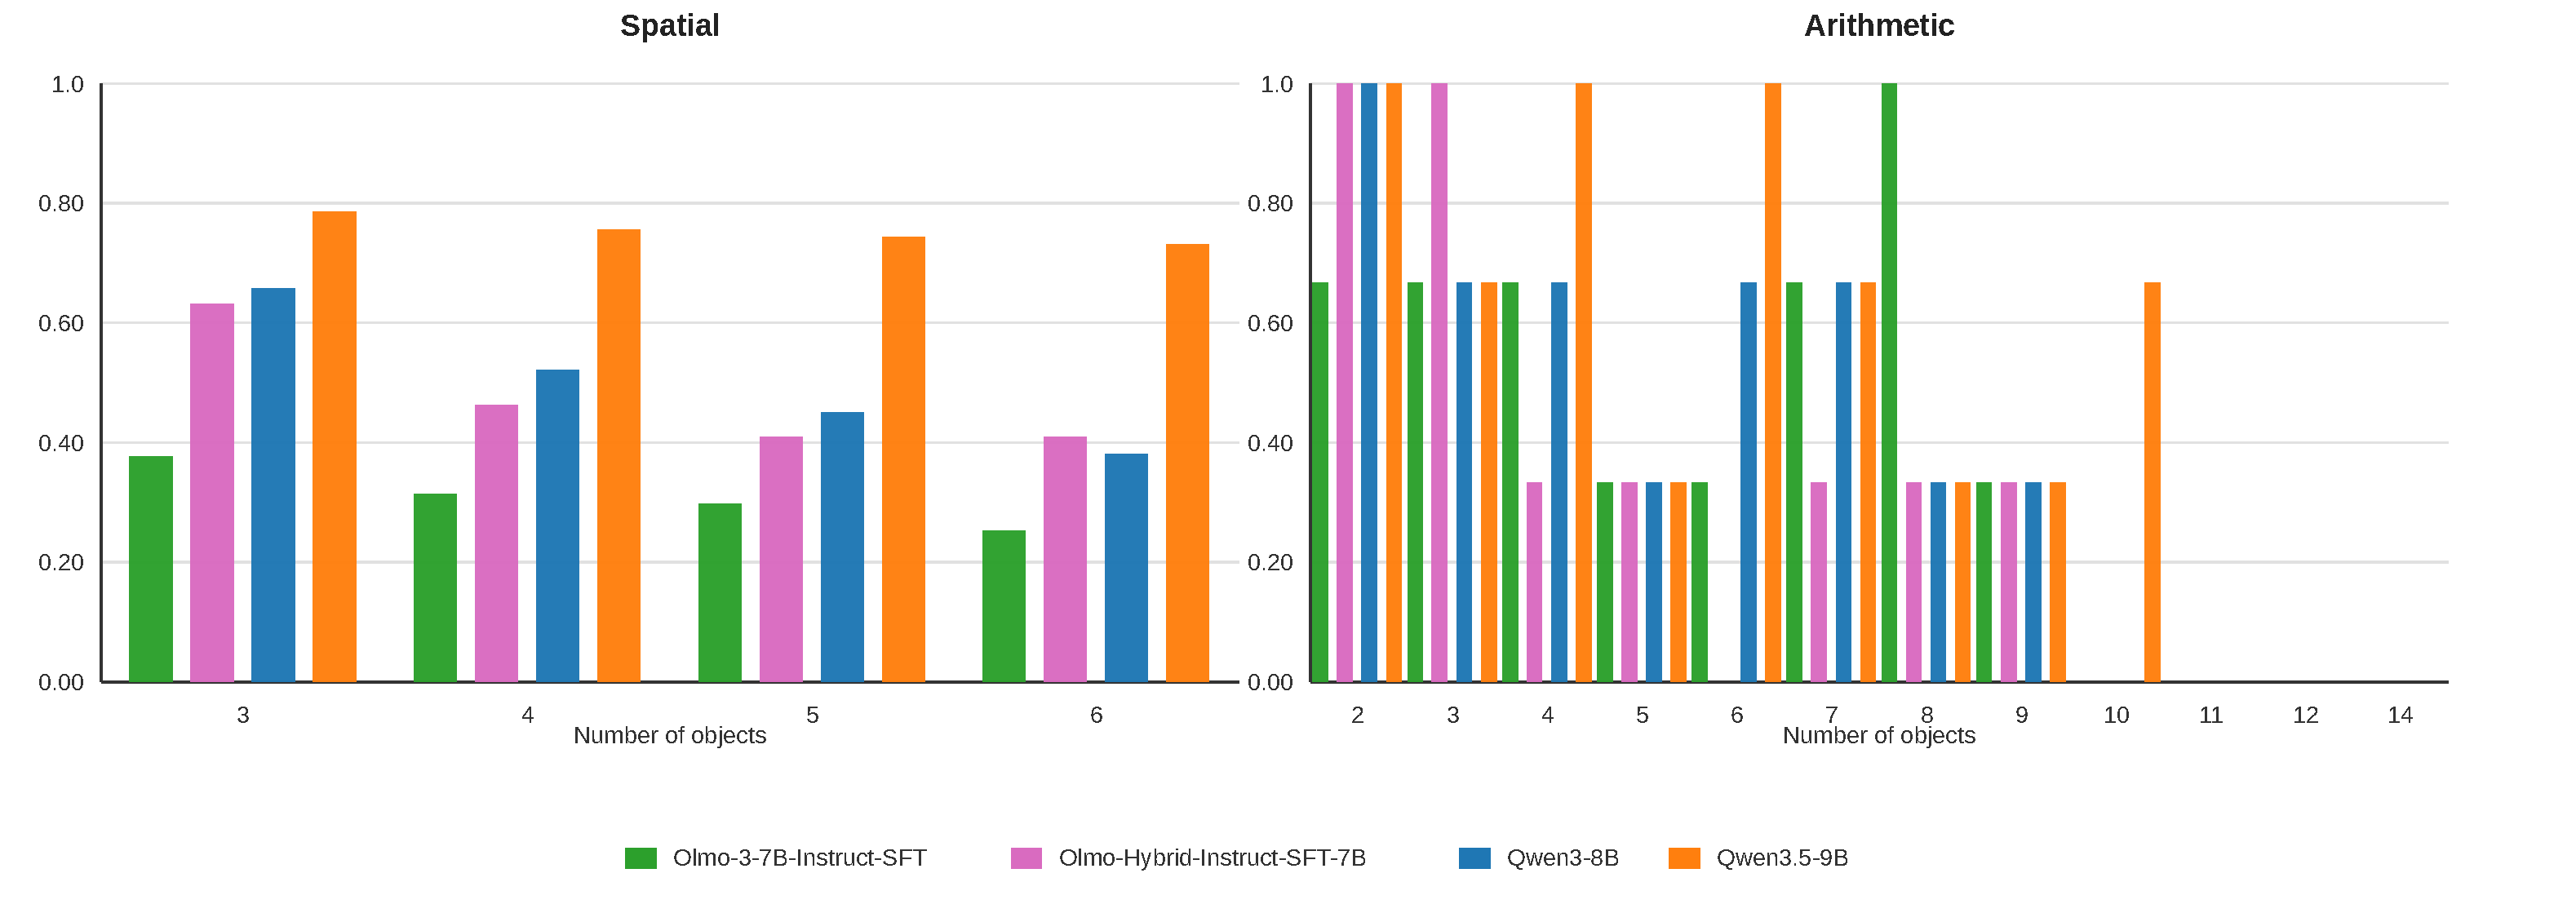
\includegraphics[width=0.9\linewidth]{assets/colored_objects/baselines_bottom_row.pdf}
    \caption{Baseline accuracy on the Colored Objects subtasks \texttt{spatial} and \texttt{arithmetic}. The x-axis shows the number of objects in the prompt, and the y-axis shows accuracy. Bars compare Olmo-3-7B-Instruct-SFT, Olmo-Hybrid-Instruct-SFT-7B, Qwen3-8B, and Qwen3.5-9B within each object-count bin.}
    \label{fig:baselines2}
\end{figure}

\begin{figure}[t]
    \centering
    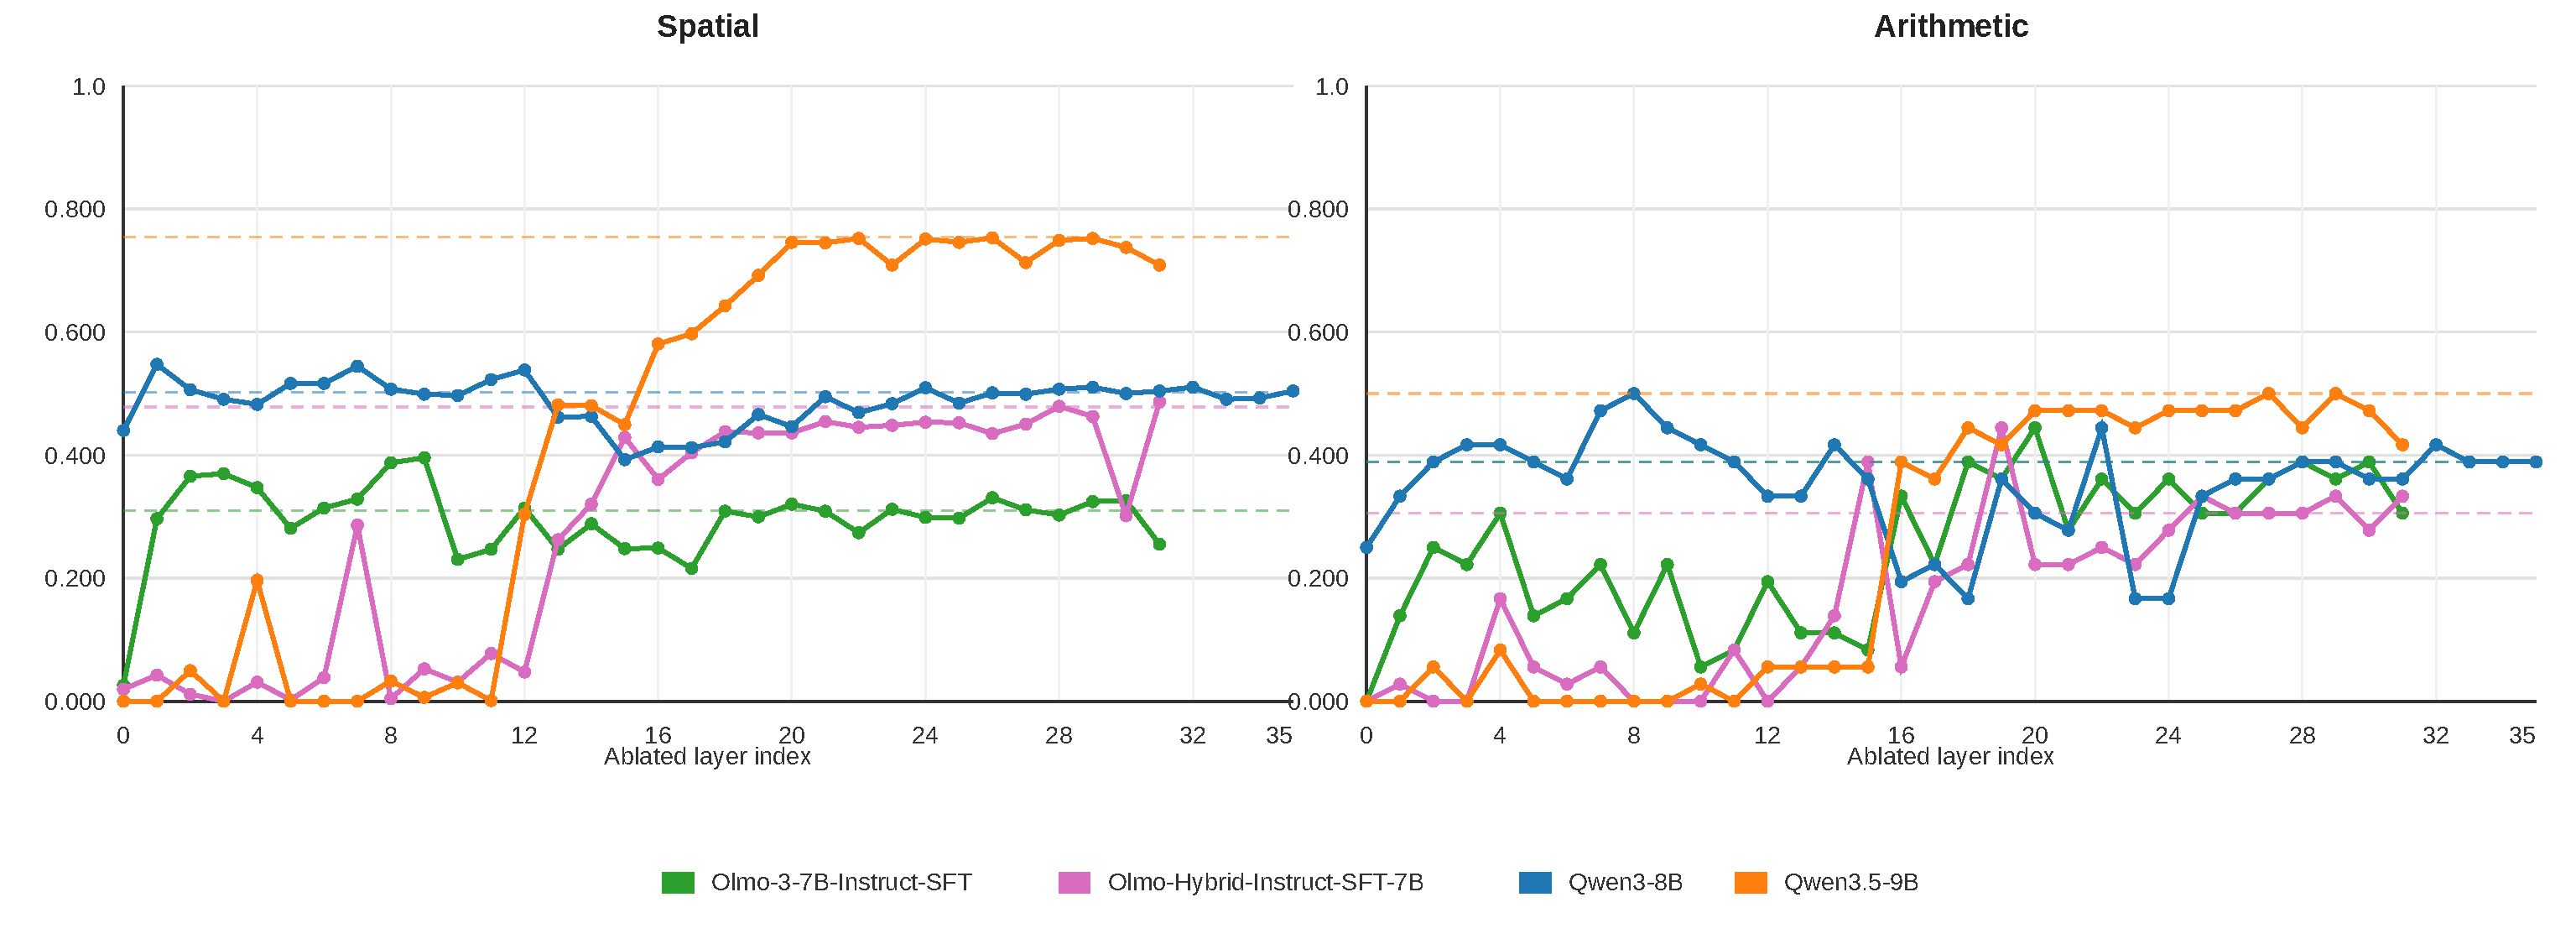
\includegraphics[width=0.9\linewidth]{assets/colored_objects/ablations_bottom_row.pdf}
    \caption{Per-layer ablation accuracy on the Colored Objects subtasks \texttt{spatial} and \texttt{arithmetic}. The x-axis shows the index of the ablated layer, and the y-axis shows accuracy after ablation. Dashed horizontal lines indicate each model's baseline accuracy without ablation.}
    \label{fig:ablations2}
\end{figure}

\section{Clinical Task}
\label{sec:clinical_data_preprocessing}

\subsection{Data Preprocessing}
For the eICU cohort, we extracted data from the \texttt{patient}, \texttt{diagnosis}, \texttt{treatment}, \texttt{medication}, \texttt{lab}, and \texttt{apacheApsVar} tables. In preparation for downstream predictive tasks (which are anchored 12 hours post-admission), we applied rigorous filtering criteria to the \texttt{patient} table. Patient age strings (e.g., ``> 89'') were parsed into integers, and we excluded patients younger than 18 or older than 89 years. Length of stay (LoS) was calculated by subtracting the \texttt{hospitaladmitoffset} from the \texttt{hospitaldischargeoffset}. We excluded visits lasting longer than 720 hours (30 days) and visits shorter than 12 hours. By anchoring the relational joins on the laboratory table (\texttt{patientunitstayid}), we established a final pretraining eICU cohort of 195,691 unique ICU stays.
We extracted age, gender, and ethnicity directly from the \texttt{patient} table.
We filtered for laboratory result types with at least 10,000 instances across the cohort to reduce sparse feature dimensions. For duplicate lab result types within a single patient stay, the total values were summed. We pivoted the data to form a feature matrix where each column represents a specific lab test, and entirely missing laboratory records for a stay were filled with zeros. Acute physiology scores (e.g., motor, verbal, meds, urine) were additionally extracted from the \texttt{apacheApsVar} table and retained as continuous features.
Because the eICU dataset relies heavily on structured medical codes rather than free text, we aggregated \texttt{diagnosis}, \texttt{treatment}, and \texttt{medication} strings. For each table, strings were grouped by \texttt{patientunitstayid} and concatenated using a pipe delimiter (\texttt{|}). We extracted the unique set of clinical events per stay and generated one-hot encoded dummy variables. To ensure computational feasibility and robust representation, we calculated the total frequency of each dummy variable across the cohort and dropped any clinical event present in fewer than 5\% of total visits.

For the eICU dataset, we anchored the cohort on the presence of valid laboratory measurements and applied the clinical inclusion criteria (age $\ge$ 18 and < 90, Length of Stay between 12 and 720 hours). This yielded an unseen fine-tuning pool of 58,538 stays. We defined two targets: Length of Stay (LoS, continuous regression in hours) and In-Hospital Mortality (binary classification).

To format the tabular eICU dataset for sequential modeling, we transformed relational EHR tables into temporally binned event sequences. Patient trajectories were partitioned into non-overlapping 12-hour windows (720 minutes) anchored to their admission time. 

Within each 12-hour bin, events were grouped by modality (demographics, diagnosis, treatment, medication, lab, and acute physiology scores). Missing continuous features within a bin were ignored, while recorded values were aggregated into modality-specific vectors:
\begin{itemize}
    \item \textbf{Laboratory Measurements:} Multiple readings of the same lab test within a bin were averaged.
    \item \textbf{Categorical/Event Modalities:} Binary indicators (e.g., diagnoses, medications) were clamped to a maximum value of $1.0$.
\end{itemize}
All aggregated vectors were subsequently normalized using a sign-preserved log-transformation, $f(x) = \text{sgn}(x) \log(1 + |x|)$. Sequences were appended with a learnable \texttt{[PREDICT]} token after every other temporal step to transparently model the decision update process. 



\subsection{Sequence Modeling}
Our architecture uses modality-specific encoders to map the precomputed vectors into a shared embedding space, which is then projected into the language model's hidden dimension. See \ref{fig:clinical sequence_modeling} for a visualization of the setup.

\textbf{Modality Encoders:} Each modality is processed by an independent Multilayer Perceptron (MLP) parameterized by an input dimension dynamically inferred from the dataset. The encoder maps inputs to an embedding dimension of $D=256$ using the following sequence: Linear $\to$ LayerNorm $\to$ ReLU $\to$ Dropout($0.3$) $\to$ Linear $\to$ LayerNorm. 

\textbf{LLM Integration and Projection:} The resulting embeddings (along with the \texttt{[PREDICT]} token embedding) are routed through an input projection module consisting of: Linear($256, D_{\text{hidden}}$) $\to$ GELU $\to$ Dropout($0.3$) $\to$ Linear($D_{\text{hidden}}, D_{\text{hidden}}$). This maps the features into the latent space of the frozen Large Language Model (LLM) backbone. 

\textbf{Classification Head:} The final hidden state corresponding to the \texttt{[PREDICT]} token is extracted and passed through a classification head: Linear($D_{\text{hidden}}, 512$) $\to$ ReLU $\to$ Dropout($0.5$) $\to$ Linear($512, \text{num\_classes}$).

\begin{figure*}
	\centering
	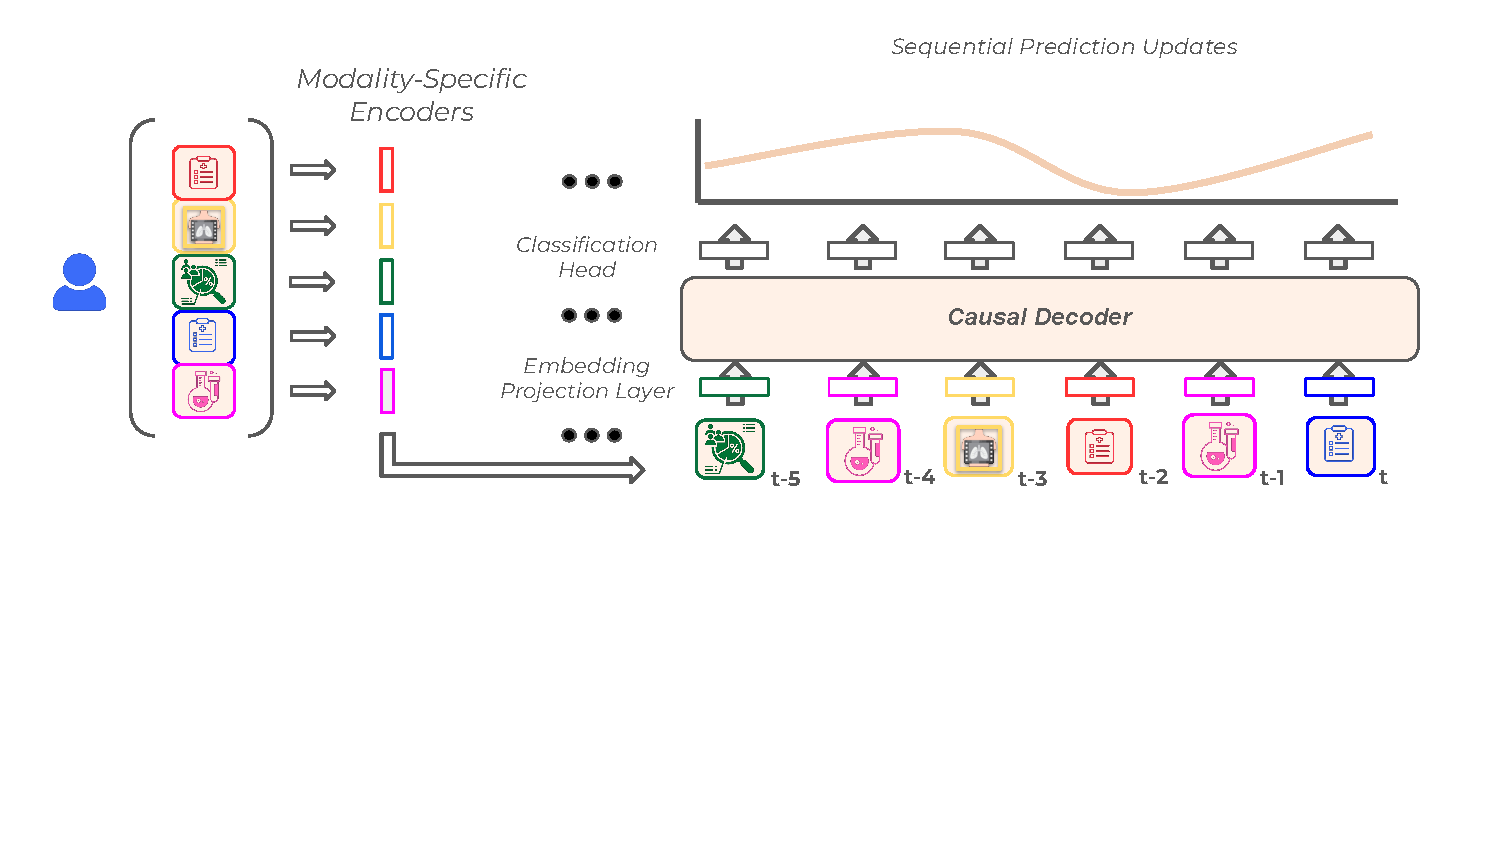
\includegraphics[width=0.85\linewidth]{assets/img/clinical_sequence_modeling.pdf}
	\caption{Overview of clinical sequence modeling architecture. We pass the raw eICU patient data through modality-specific encoders, then auto-regressively input them to a causal decoder in temporal order.} 
	\label{fig:clinical sequence_modeling}
\end{figure*}

\subsection{Training Details}
We evaluated the six LLM backbones across pure transformer and hybrid architectures referenced in \ref{}. 

To ensure memory-efficient training, all LLM backbones were quantized to 4-bit NormalFloat (NF4) with double quantization and bfloat16 compute precision using BitsAndBytes. We applied Low-Rank Adaptation (LoRA) across all linear target modules (\texttt{target\_modules="all-linear"}) , and LoRA hyperparameters were fixed at rank $r=16$, $\alpha=32$, and a dropout of $0.1$. Throughput was maximized using Flash Attention 2 and gradient checkpointing.

Models were optimized using the 8-bit AdamW optimizer. For hyperparameter tuning, we executed a grid search sweeping learning rates across $\{1\times 10^{-5}, 3\times 10^{-5}, 5\times 10^{-5}\}$ and weight decay across $\{0.01, 0.05, 0.1\}$. Gradients were clipped to a maximum norm of $1.0$.
For the in-hospital mortality task, we formulated it as a binary classification task. Models were trained using Binary Cross-Entropy with Logits loss (\texttt{BCEWithLogitsLoss}), applying a positive class weight of $10.76$ to counter class imbalance.
   

All configurations utilized a per-device batch size of 2 with 8 gradient accumulation steps (effective batch size of 16). Models were trained for a maximum of 40 epochs, with an early stopping patience of 5 epochs monitored against the validation AUROC. All models were trained on NVIDIA 3090 RTX GPUs.

\clearpage

\subsection{Clinical Sequence Modeling Ablation Studies}
\begin{figure*}[t]
    \centering
    % Row 1: OLMo Models
    \begin{subfigure}[b]{0.48\textwidth}
        \centering
        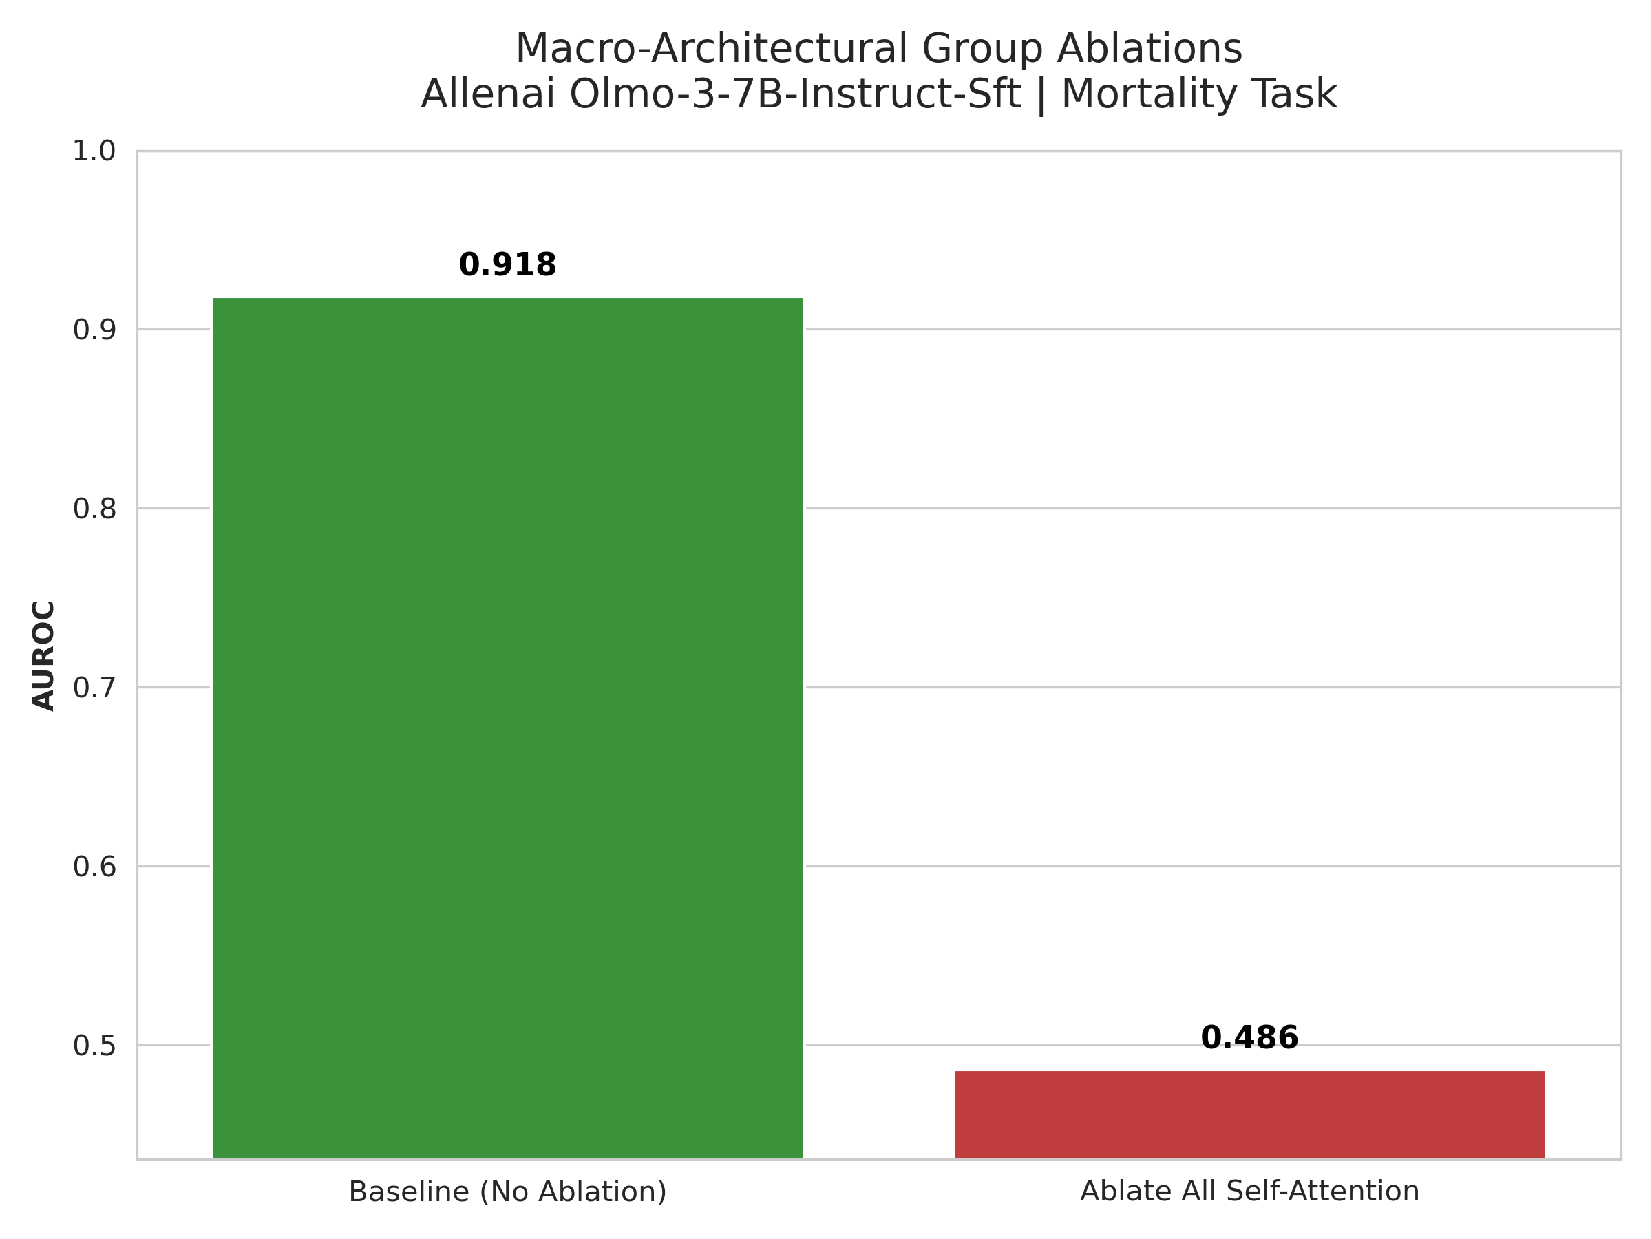
\includegraphics[width=\textwidth]{assets/img/allenai_Olmo-3-7B-Instruct-SFT_mortality_task_group_ablations.pdf}
        \caption{OLMo-3-7B (Transformer)}
        \label{fig:seq_olmo_base}
    \end{subfigure}
    \hfill
    \begin{subfigure}[b]{0.48\textwidth}
        \centering
        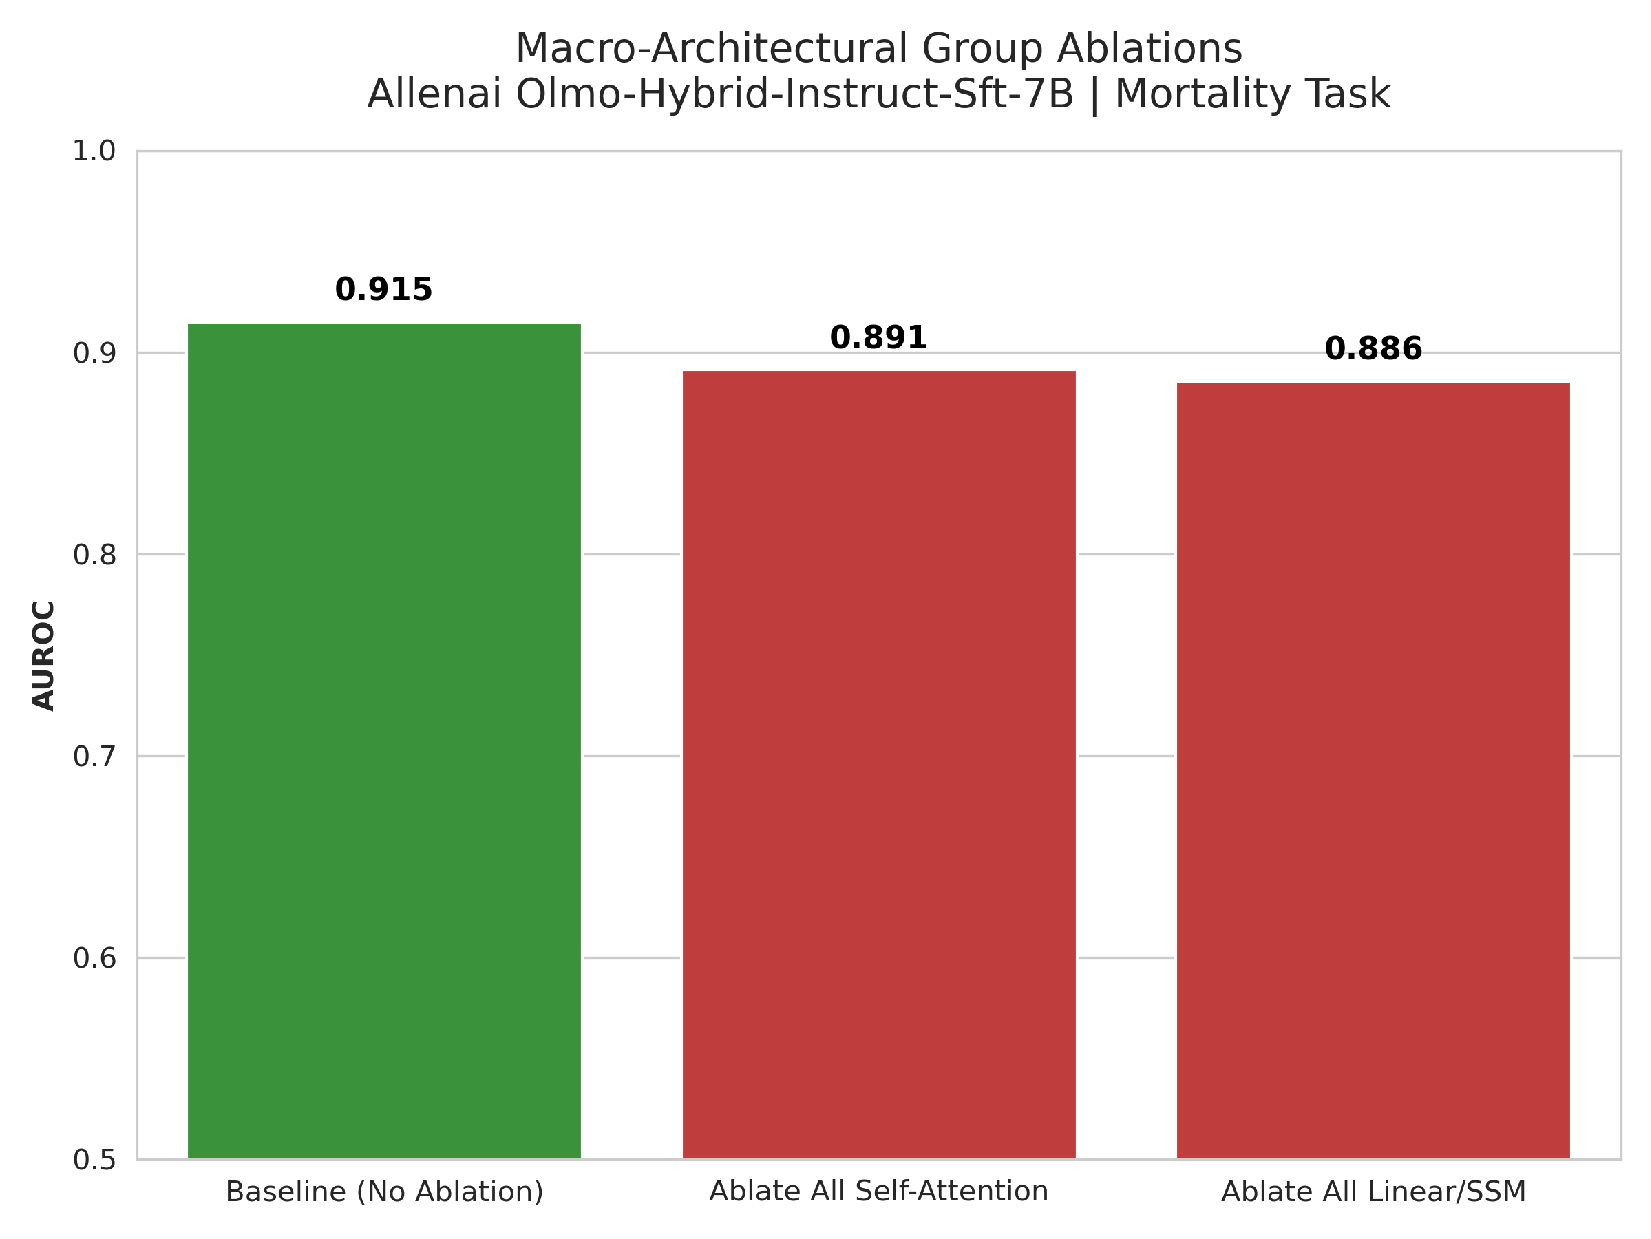
\includegraphics[width=\textwidth]{assets/img/allenai_Olmo-Hybrid-Instruct-SFT-7B_mortality_task_group_ablations.pdf}
        \caption{OLMo-Hybrid-7B}
        \label{fig:seq_olmo_hybrid}
    \end{subfigure}
    
    \vspace{1em} % Add some vertical space between rows
    
    % Row 2: Qwen 8B/9B Models
    \begin{subfigure}[b]{0.48\textwidth}
        \centering
        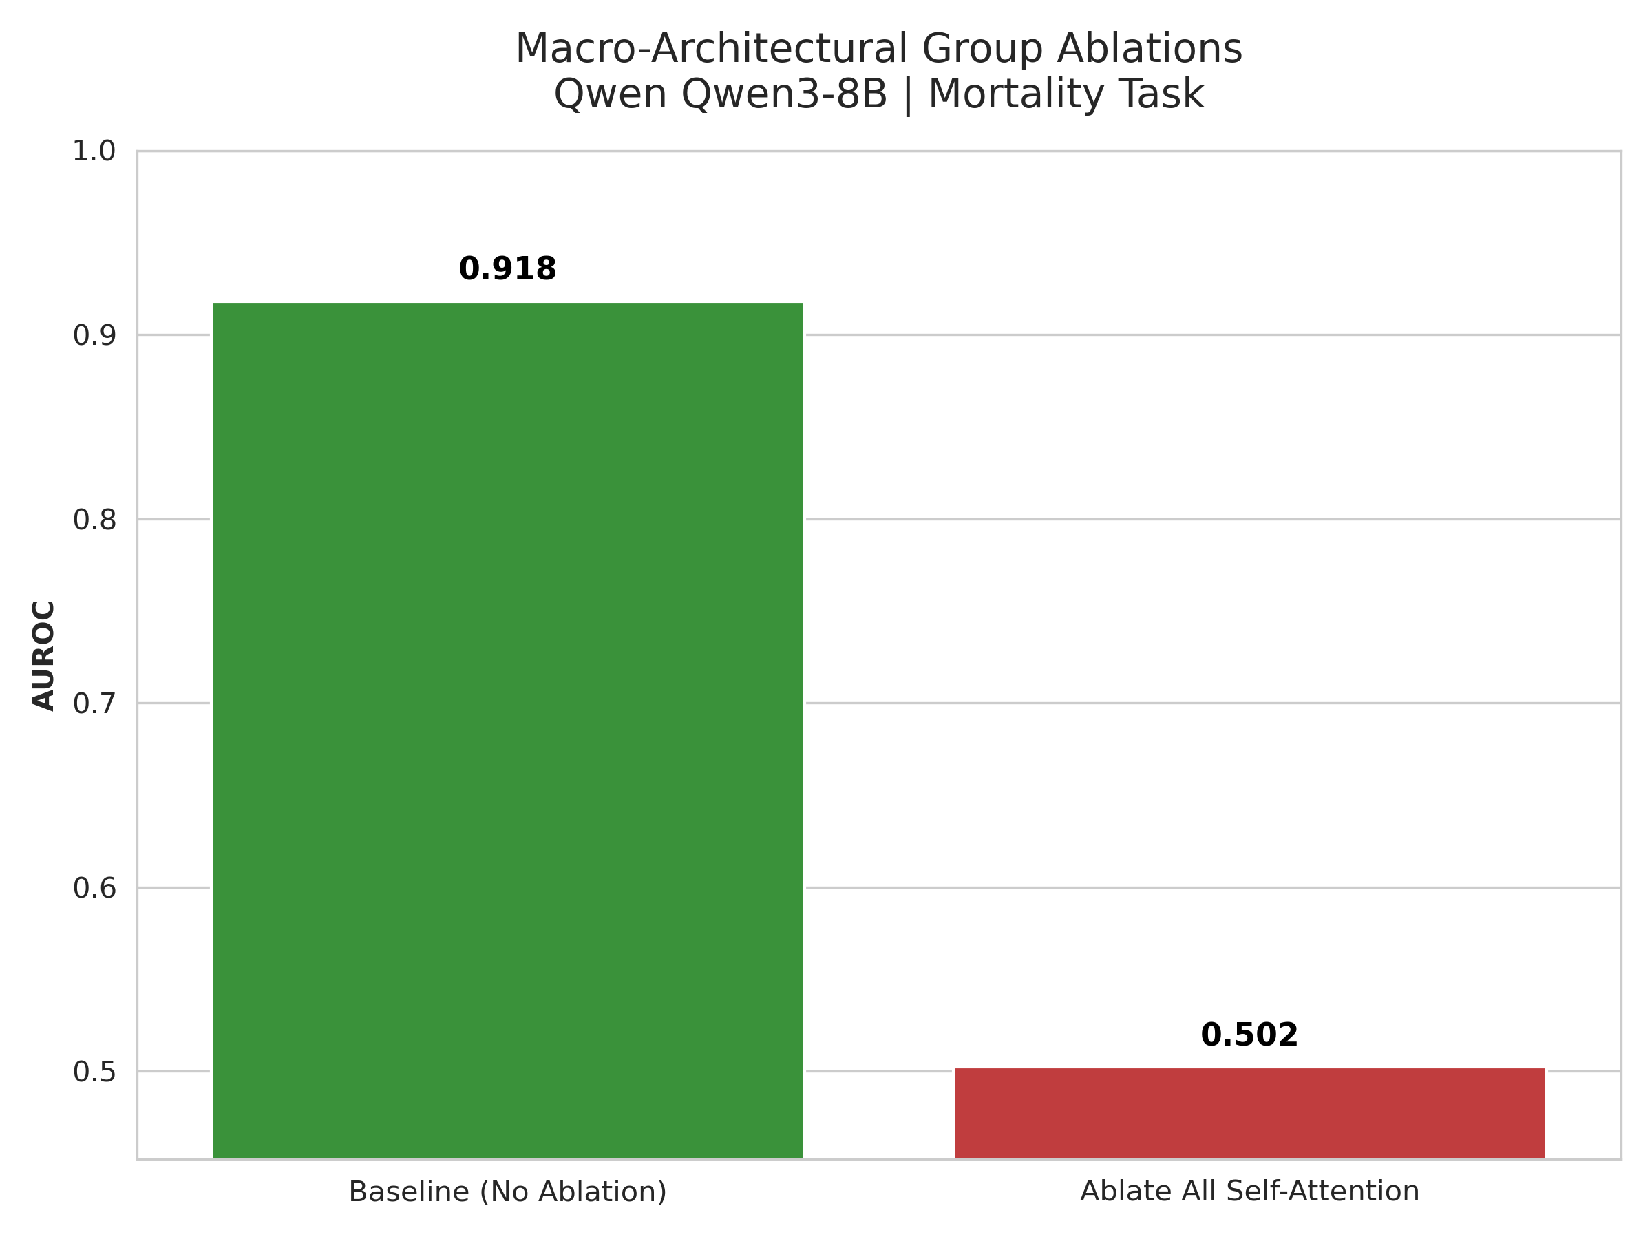
\includegraphics[width=\textwidth]{assets/img/Qwen_Qwen3-8B_mortality_task_group_ablations.pdf}
        \caption{Qwen3-8B (Transformer)}
        \label{fig:seq_qwen_8b}
    \end{subfigure}
    \hfill
    \begin{subfigure}[b]{0.48\textwidth}
        \centering
        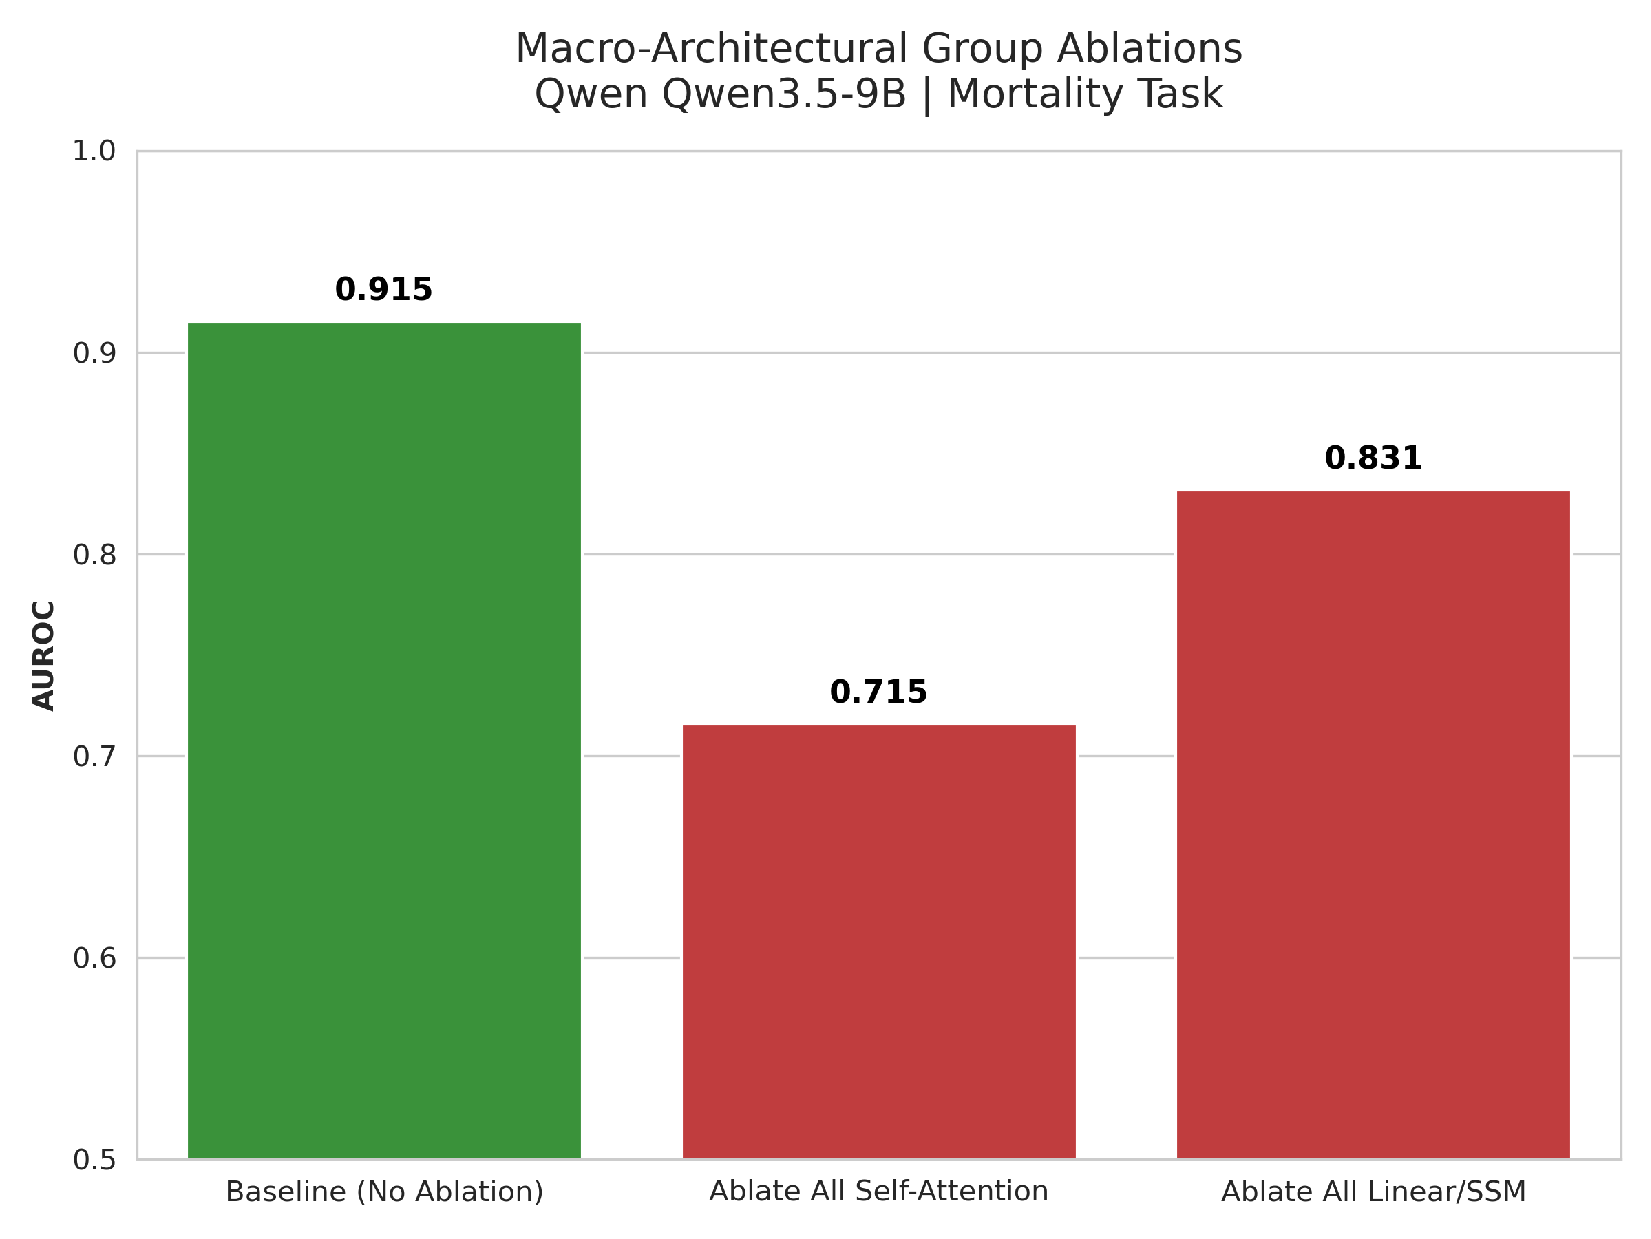
\includegraphics[width=\textwidth]{assets/img/Qwen_Qwen3.5-9B_mortality_task_group_ablations.pdf}
        \caption{Qwen3.5-9B (Hybrid)}
        \label{fig:seq_qwen_9b}
    \end{subfigure}
    
    \vspace{1em}
    
    % Row 3: Qwen 27B/32B Models
    \begin{subfigure}[b]{0.48\textwidth}
        \centering
        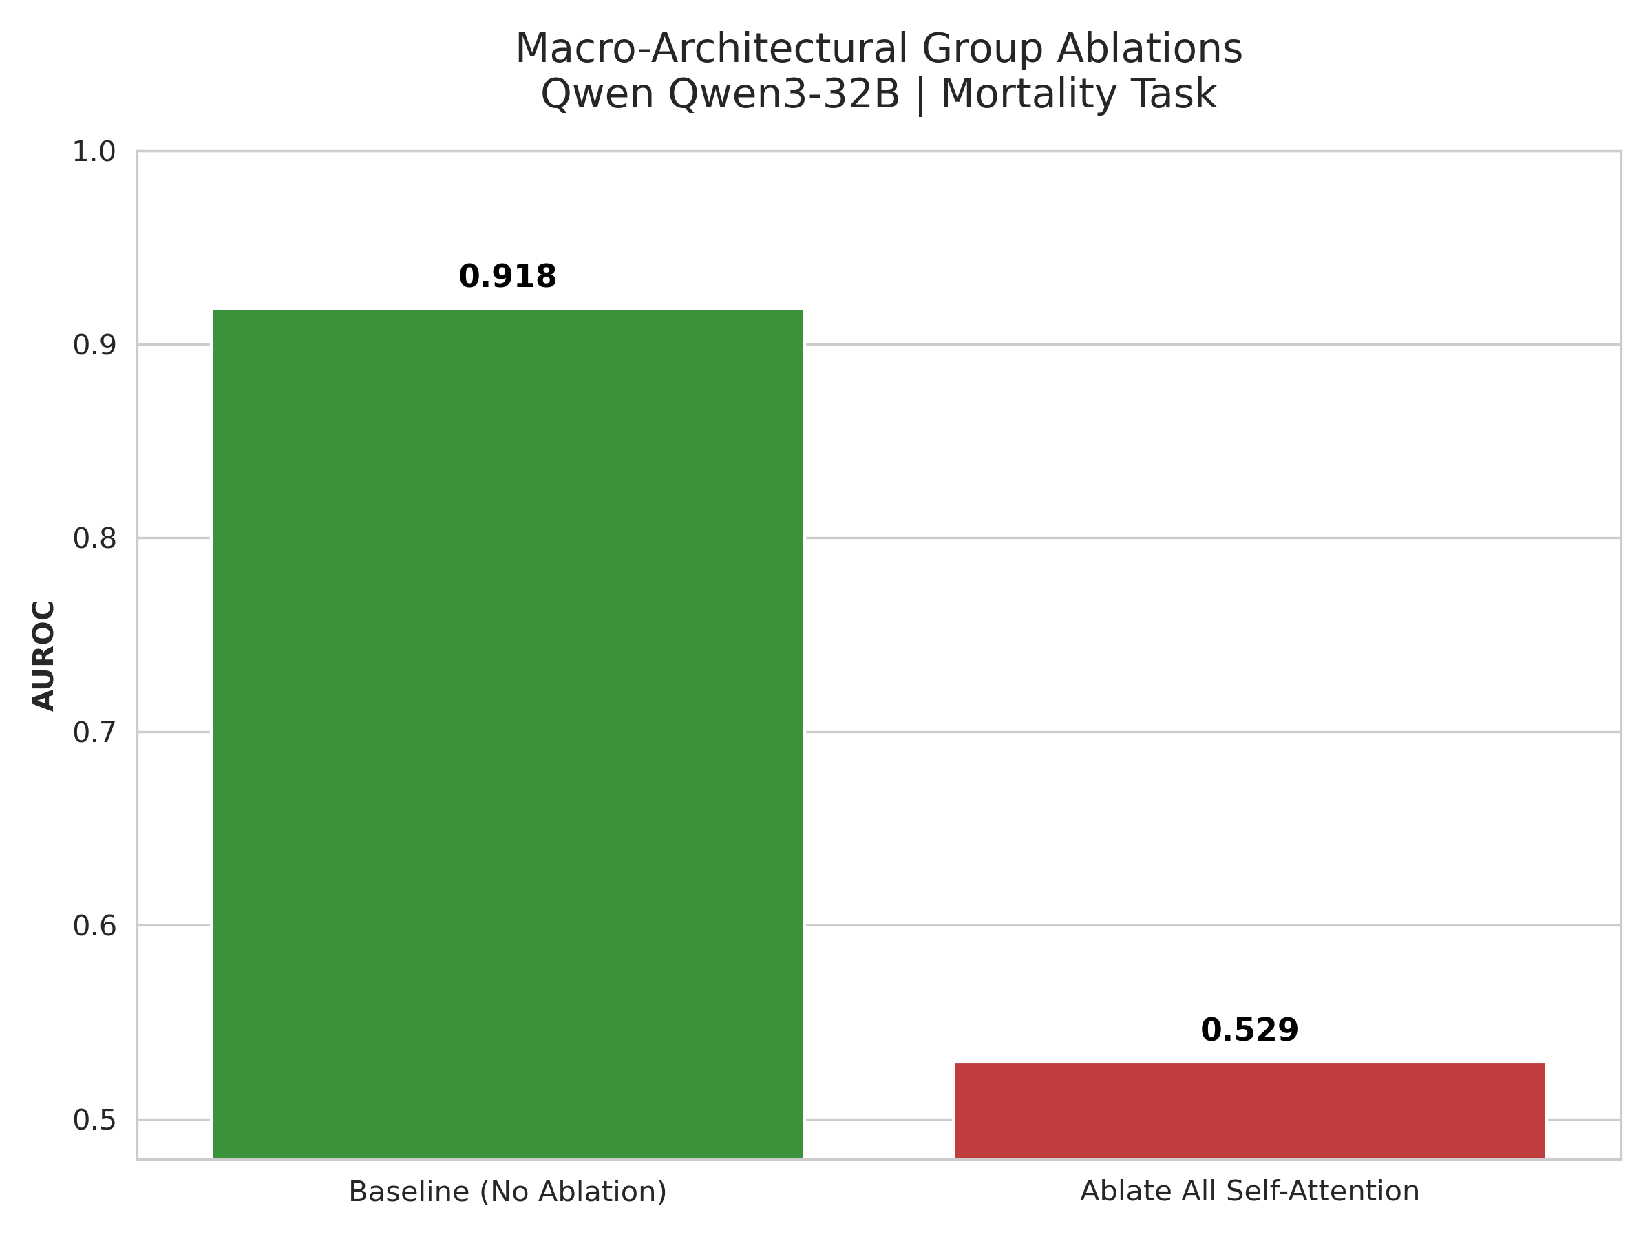
\includegraphics[width=\textwidth]{assets/img/Qwen_Qwen3-32B_mortality_task_group_ablations.pdf}
        \caption{Qwen3-32B (Transformer)}
        \label{fig:seq_qwen_32b}
    \end{subfigure}
    \hfill
    \begin{subfigure}[b]{0.48\textwidth}
        \centering
        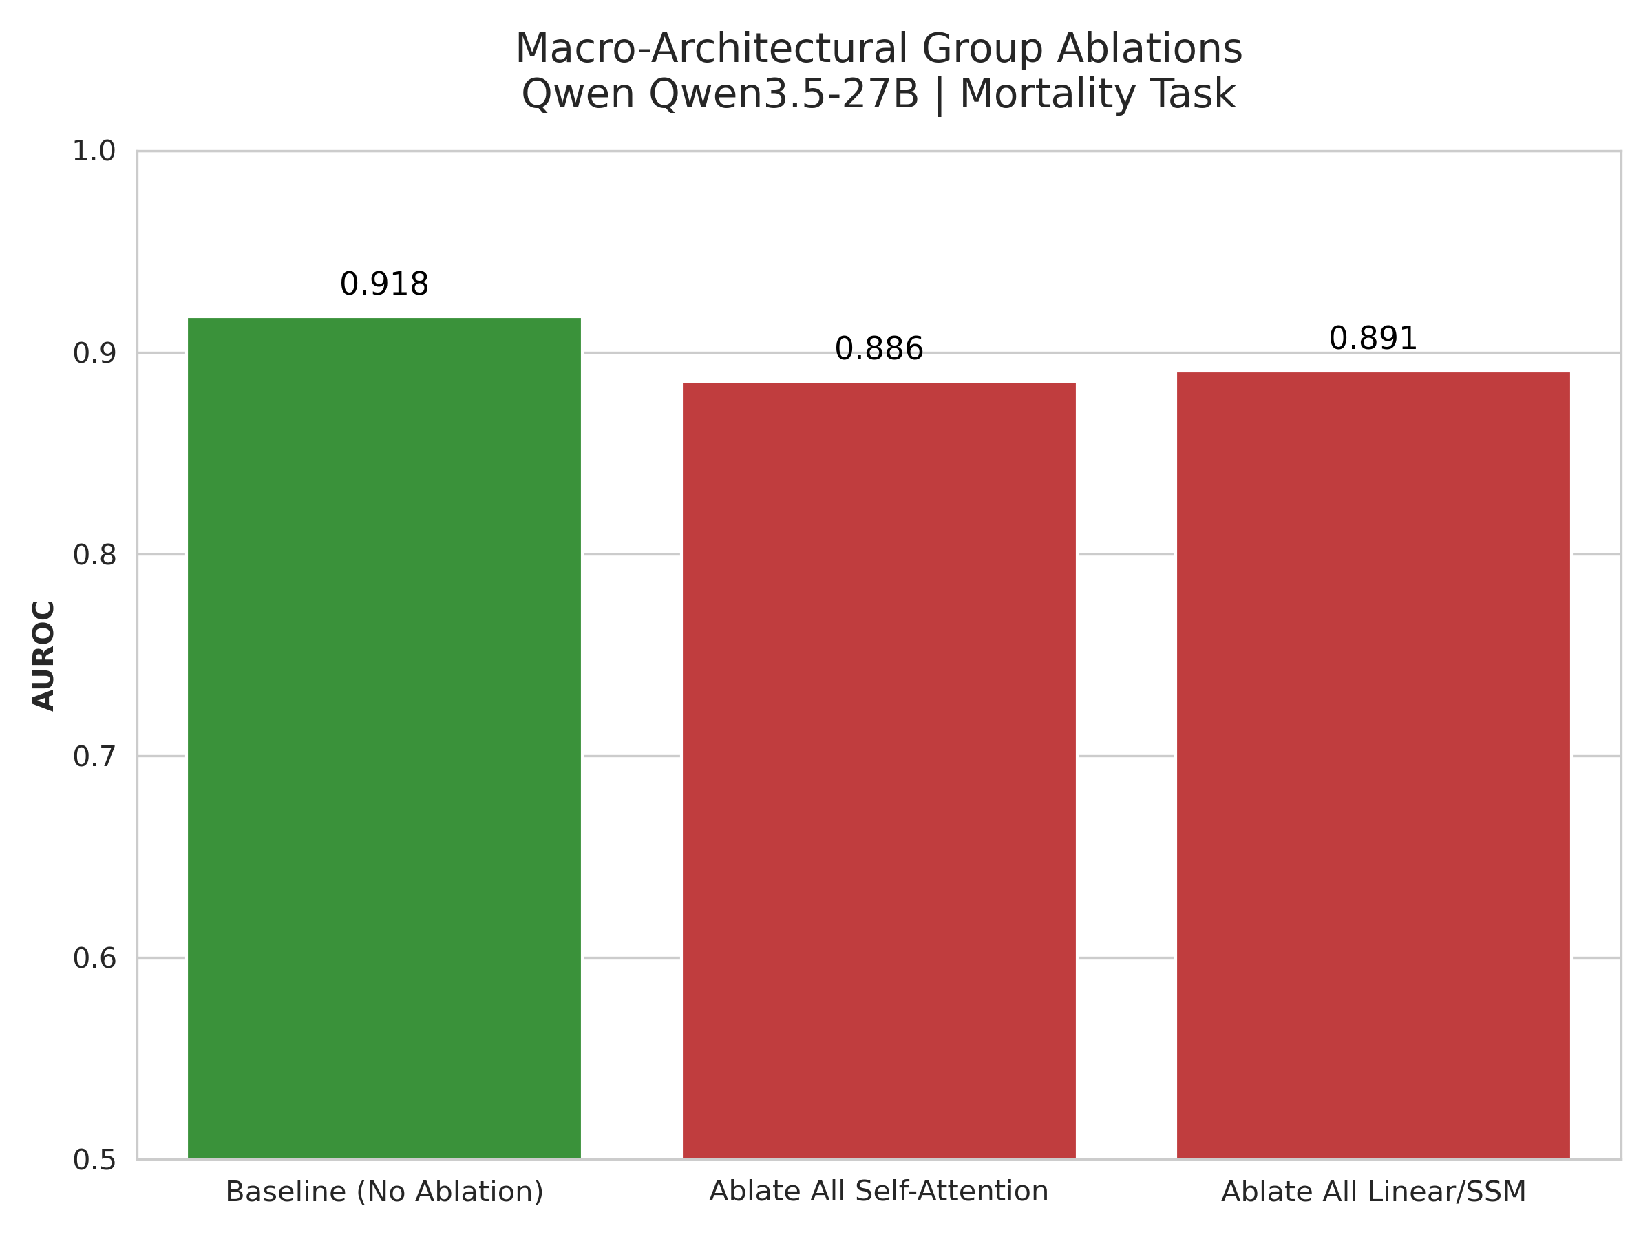
\includegraphics[width=\textwidth]{assets/img/Qwen_Qwen3.5-27B_mortality_task_group_ablations.pdf}
        \caption{Qwen3.5-27B (Hybrid)}
        \label{fig:seq_qwen_27b}
    \end{subfigure}
    
    \caption{Mechanistic Ablation Study results for the In-Hospital Mortality task.}
    \label{fig:component_ablations}
\end{figure*}

\clearpage
\begin{figure*}[t]
    \centering
    % Row 1: OLMo Models
    \begin{subfigure}[b]{0.48\textwidth}
        \centering
        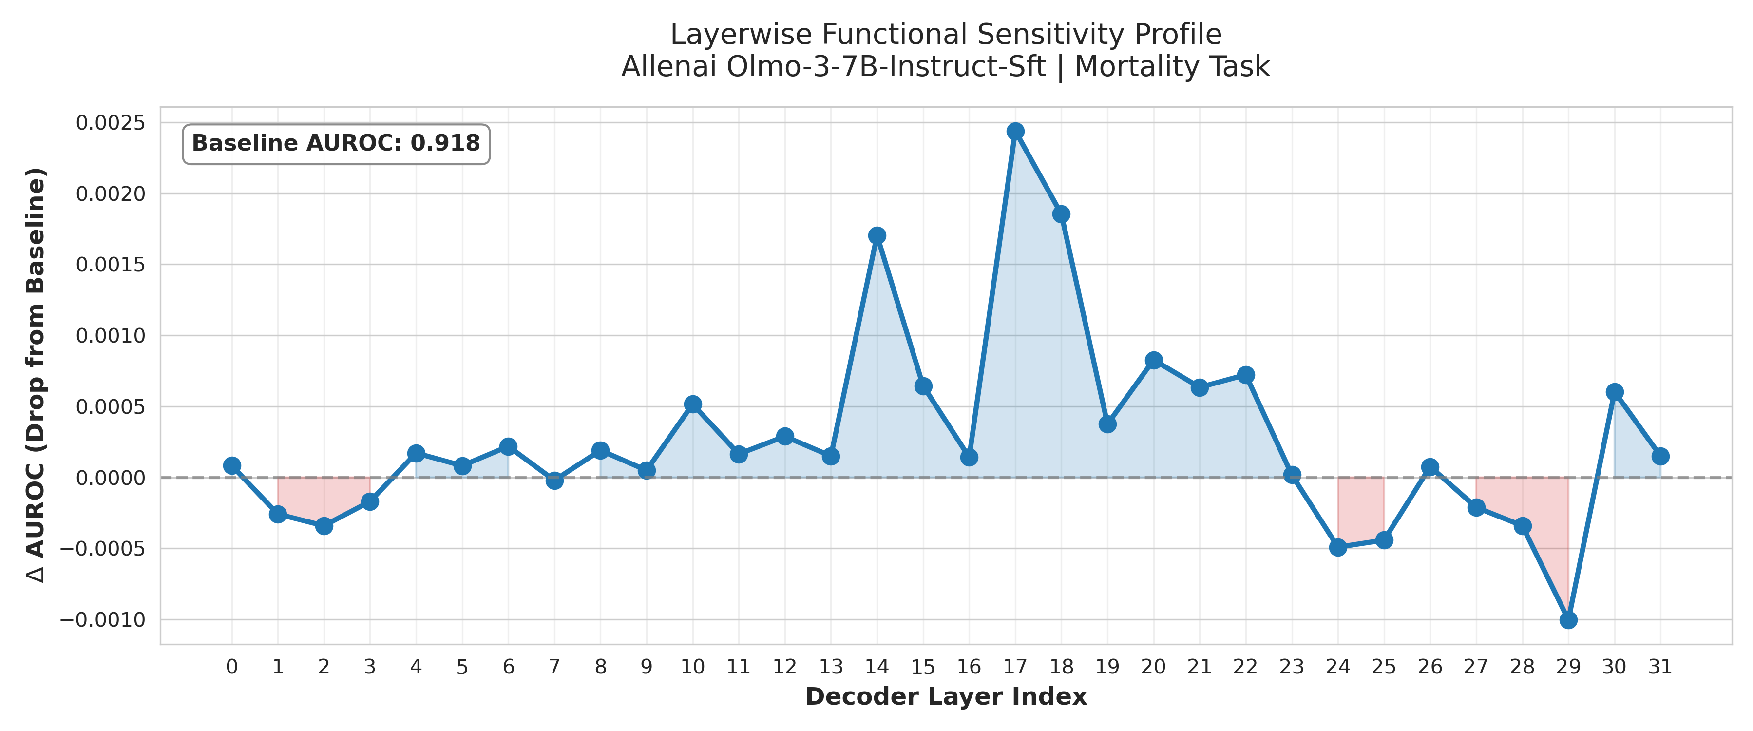
\includegraphics[width=\textwidth]{assets/img/allenai_Olmo-3-7B-Instruct-SFT_mortality_task_layerwise_sensitivity.pdf}
        \caption{OLMo-3-7B (Transformer)}
        \label{fig:seq_olmo_base}
    \end{subfigure}
    \hfill
    \begin{subfigure}[b]{0.48\textwidth}
        \centering
        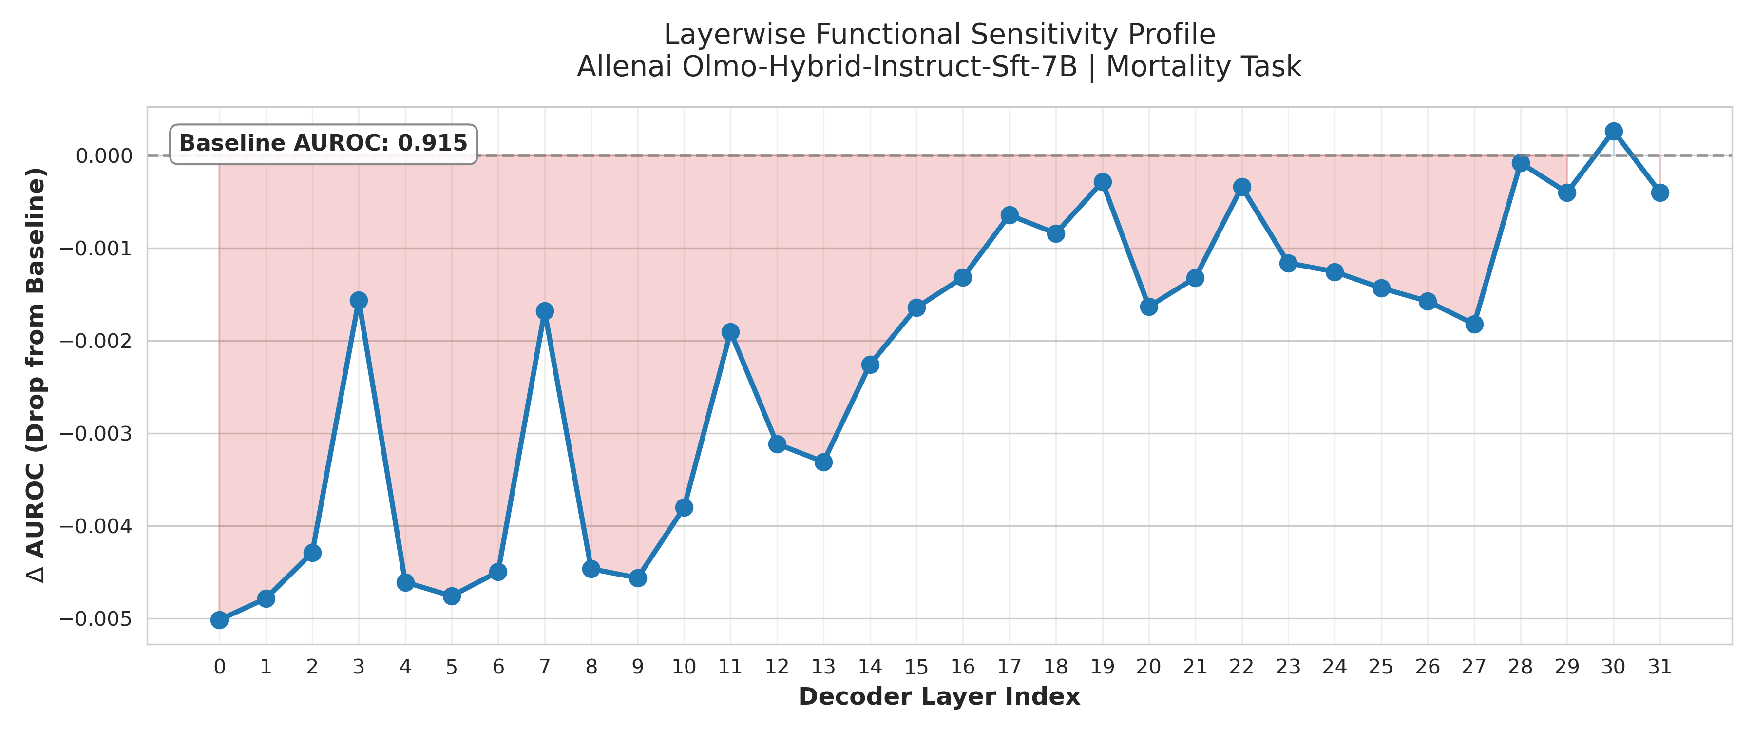
\includegraphics[width=\textwidth]{assets/img/allenai_Olmo-Hybrid-Instruct-SFT-7B_mortality_task_layerwise_sensitivity.pdf}
        \caption{OLMo-Hybrid-7B}
        \label{fig:seq_olmo_hybrid}
    \end{subfigure}
    
    \vspace{1em} % Add some vertical space between rows
    
    % Row 2: Qwen 8B/9B Models
    \begin{subfigure}[b]{0.48\textwidth}
        \centering
        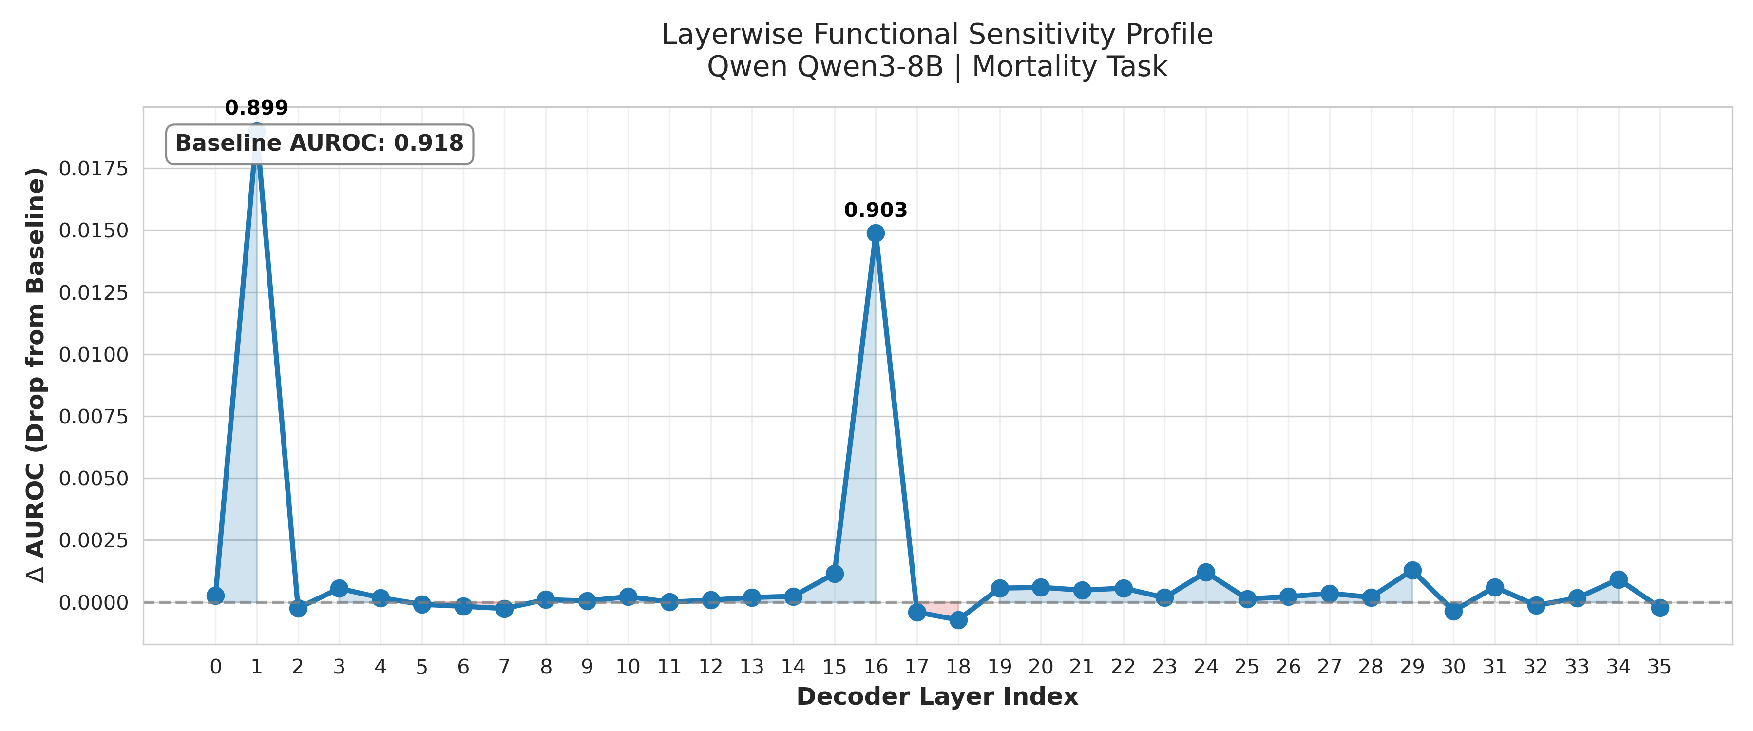
\includegraphics[width=\textwidth]{assets/img/Qwen_Qwen3-8B_mortality_task_layerwise_sensitivity.pdf}
        \caption{Qwen3-8B (Transformer)}
        \label{fig:seq_qwen_8b}
    \end{subfigure}
    \hfill
    \begin{subfigure}[b]{0.48\textwidth}
        \centering
        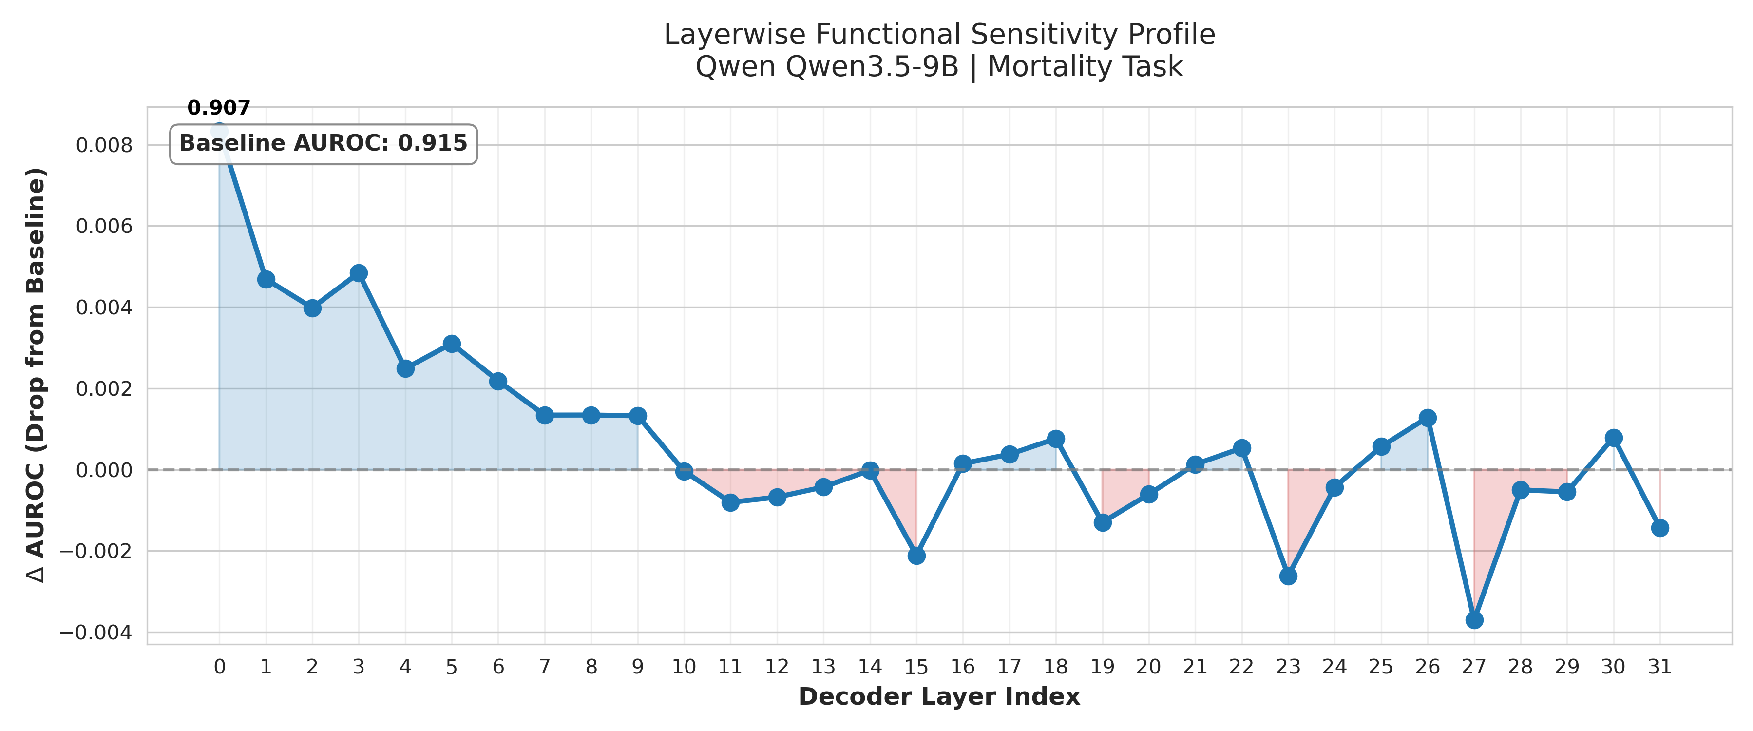
\includegraphics[width=\textwidth]{assets/img/Qwen_Qwen3.5-9B_mortality_task_layerwise_sensitivity.pdf}
        \caption{Qwen3.5-9B (Hybrid)}
        \label{fig:seq_qwen_9b}
    \end{subfigure}
    
    \vspace{1em}
    
    % Row 3: Qwen 27B/32B Models
    \begin{subfigure}[b]{0.48\textwidth}
        \centering
        \includegraphics[width=\textwidth]{}
        \caption{Qwen3-32B (Transformer) \textbf{TODO}}
        \label{fig:seq_qwen_32b}
    \end{subfigure}
        \hfill
    \begin{subfigure}[b]{0.48\textwidth}
        \centering
        \includegraphics[width=\textwidth]{}
        \caption{Qwen3.5-27B (Hybrid) \textbf{TODO}}
        \label{fig:seq_qwen_27b}
    \end{subfigure}
    
    \caption{Mechanistic Ablation Study results for the In-Hospital Mortality task.}
    \label{fig:component_ablations}
\end{figure*}

\clearpage
\begin{figure*}[t]
    \centering
    % Row 1: OLMo Models
    \begin{subfigure}[b]{0.48\textwidth}
        \centering
        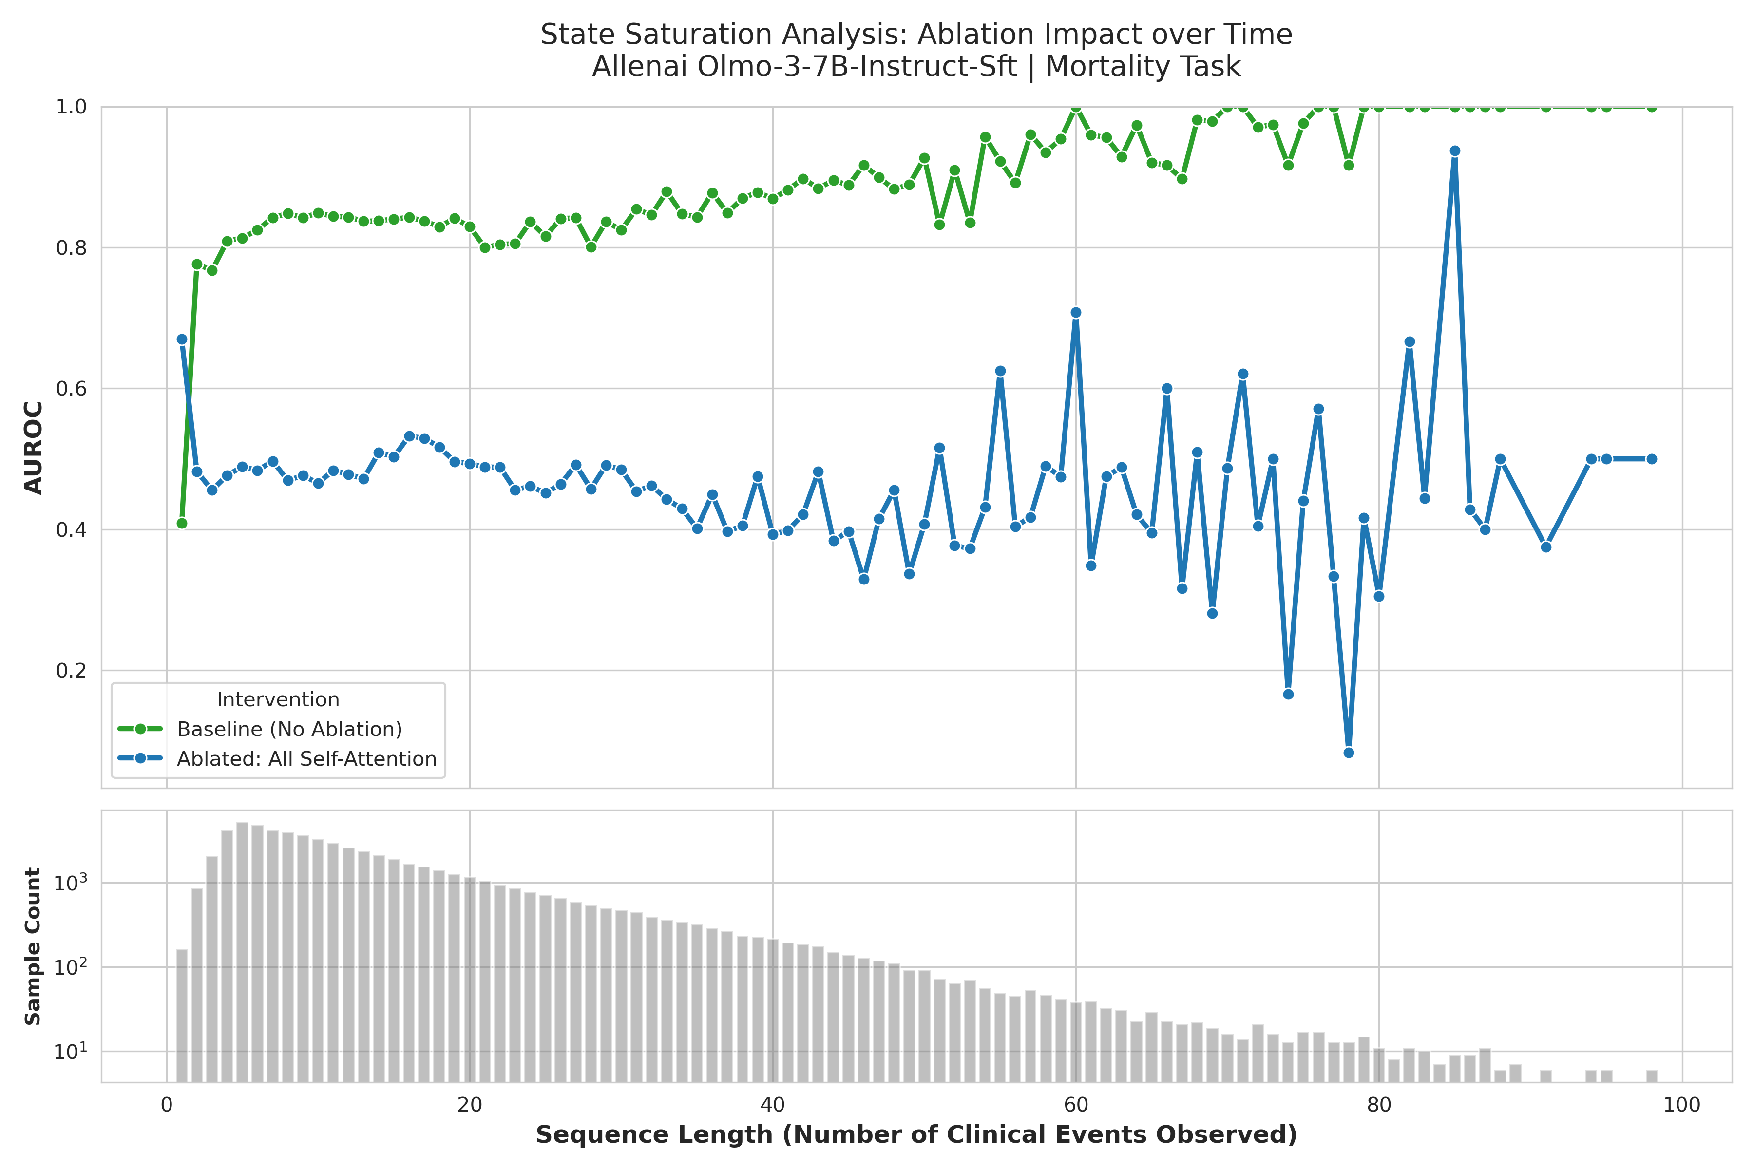
\includegraphics[width=\textwidth]{assets/img/allenai_Olmo-3-7B-Instruct-SFT_mortality_task_state_saturation.pdf}
        \caption{OLMo-3-7B (Transformer)}
        \label{fig:seq_olmo_base}
    \end{subfigure}
    \hfill
    \begin{subfigure}[b]{0.48\textwidth}
        \centering
        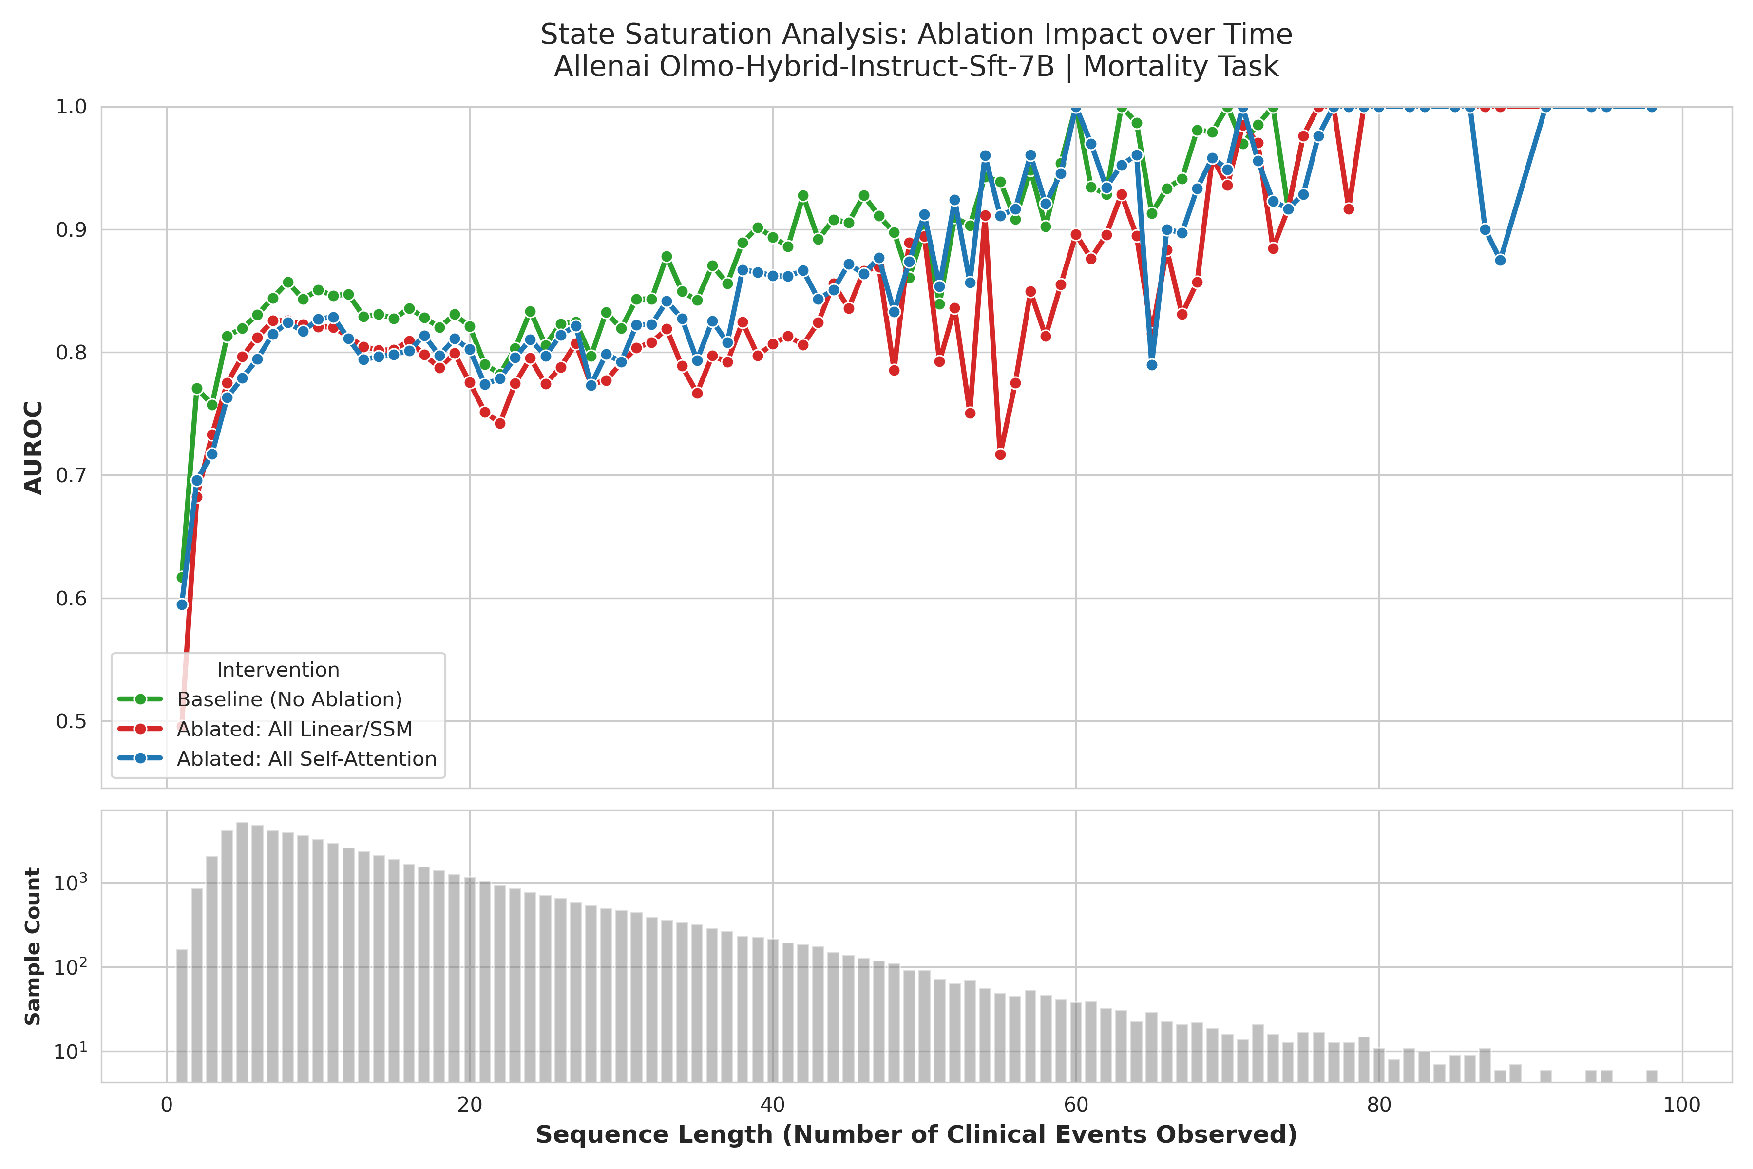
\includegraphics[width=\textwidth]{assets/img/allenai_Olmo-Hybrid-Instruct-SFT-7B_mortality_task_state_saturation.pdf}
        \caption{OLMo-Hybrid-7B}
        \label{fig:seq_olmo_hybrid}
    \end{subfigure}
    
    \vspace{1em} % Add some vertical space between rows
    
    % Row 2: Qwen 8B/9B Models
    \begin{subfigure}[b]{0.48\textwidth}
        \centering
        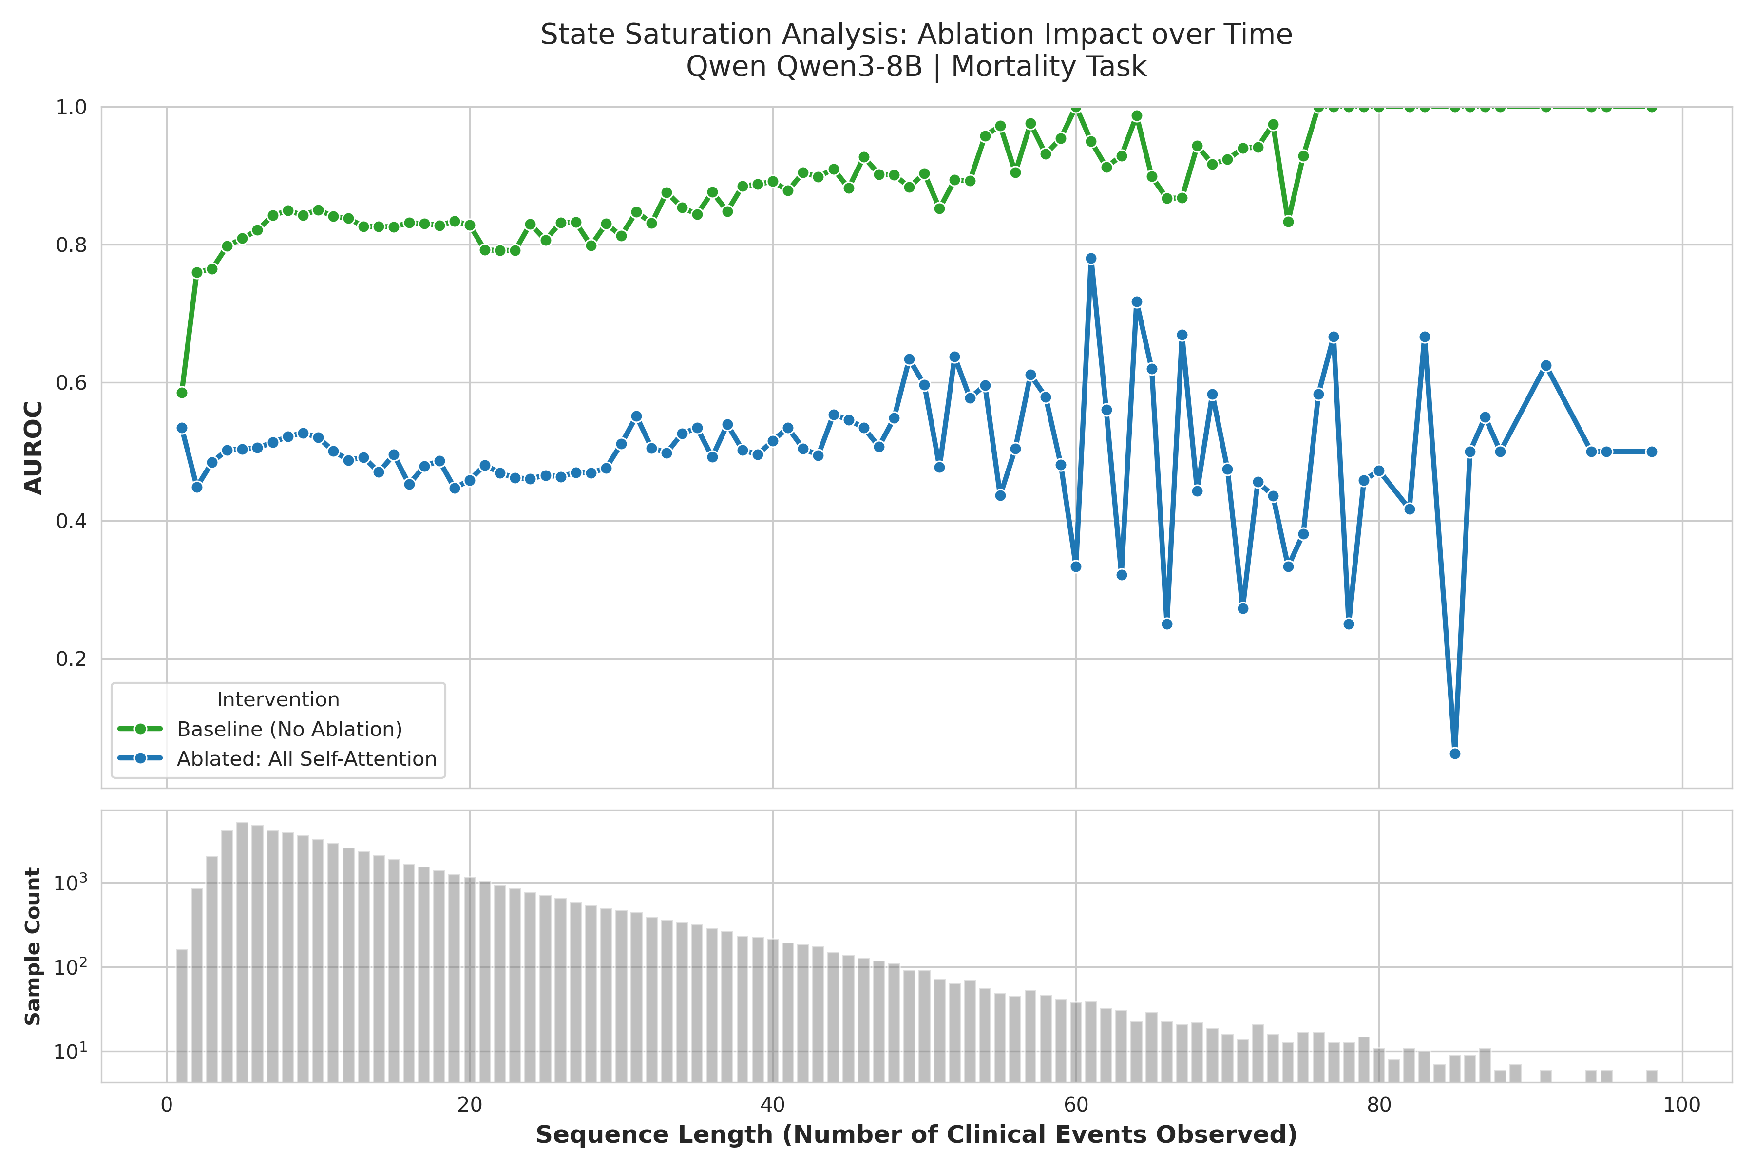
\includegraphics[width=\textwidth]{assets/img/Qwen_Qwen3-8B_mortality_task_state_saturation.pdf}
        \caption{Qwen3-8B (Transformer)}
        \label{fig:seq_qwen_8b}
    \end{subfigure}
    \hfill
    \begin{subfigure}[b]{0.48\textwidth}
        \centering
        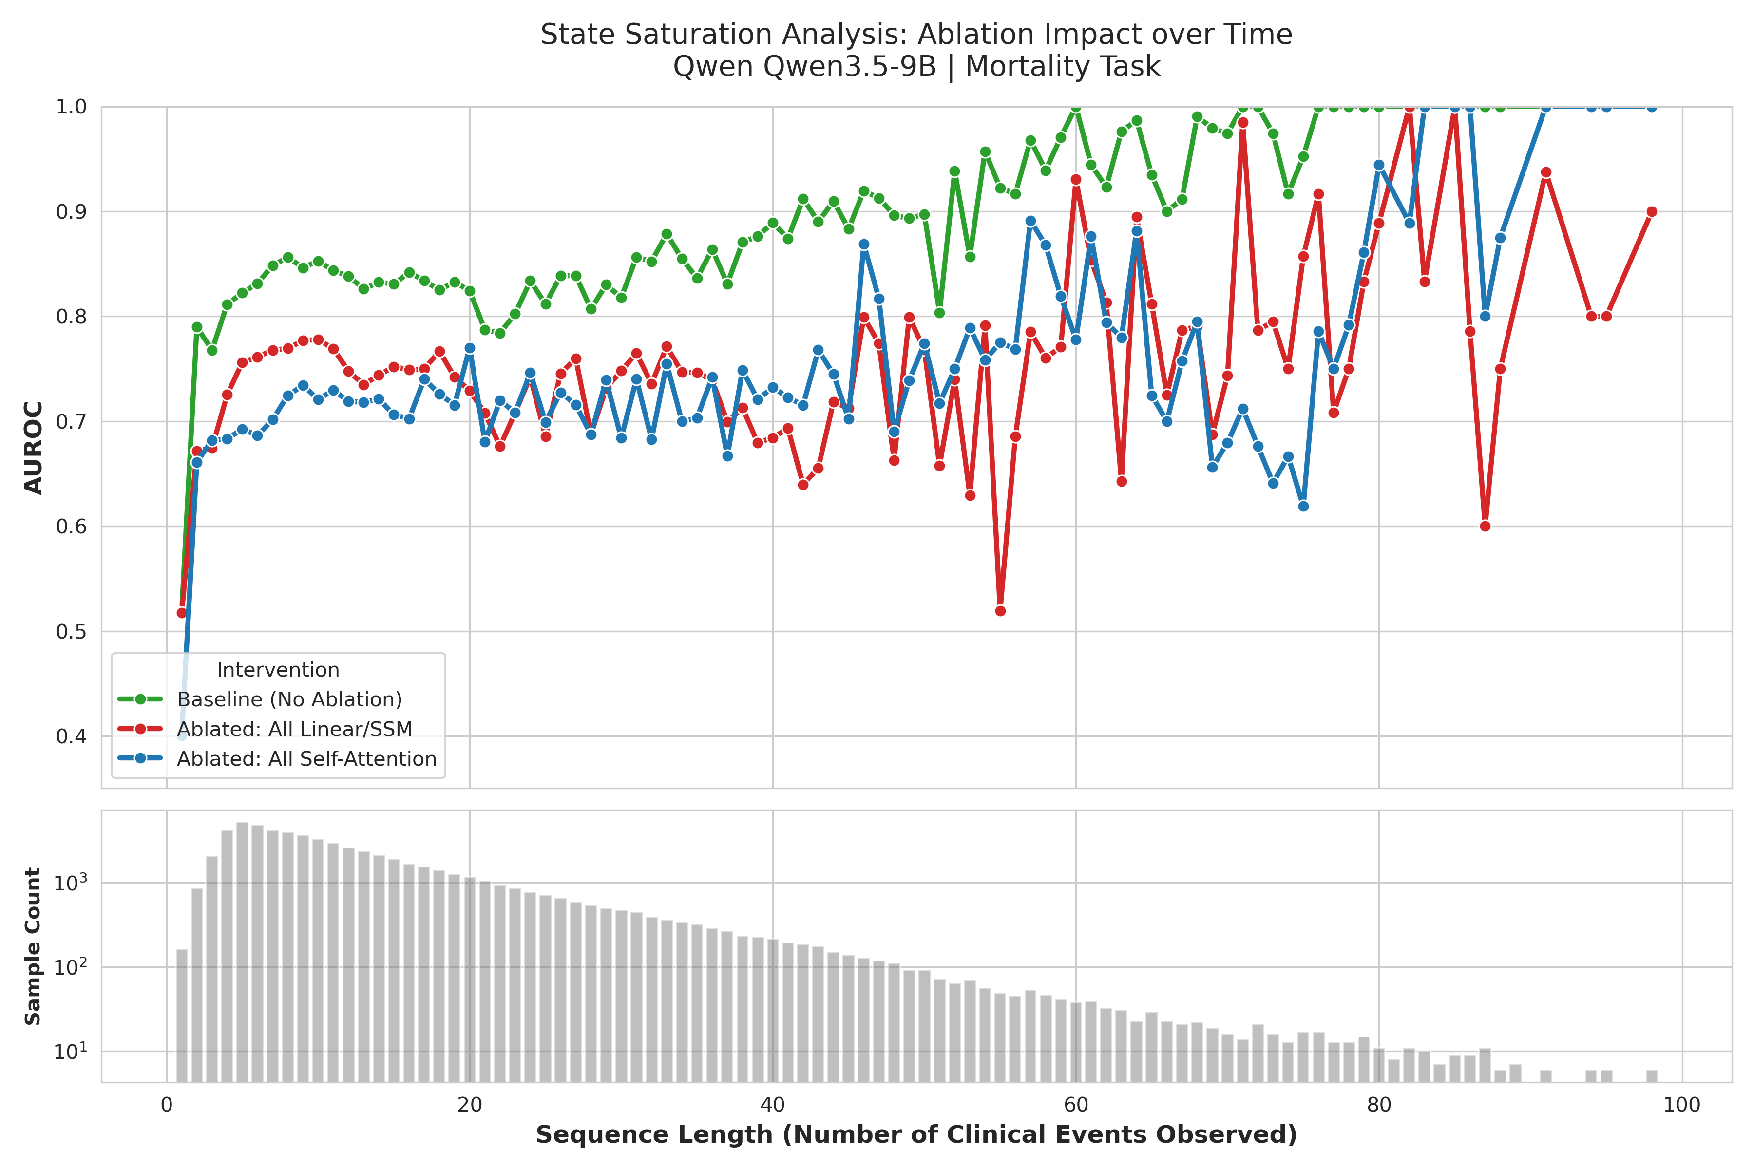
\includegraphics[width=\textwidth]{assets/img/Qwen_Qwen3.5-9B_mortality_task_state_saturation.pdf}
        \caption{Qwen3.5-9B (Hybrid)}
        \label{fig:seq_qwen_9b}
    \end{subfigure}
    
    \vspace{1em}
    
    % Row 3: Qwen 27B/32B Models
    \begin{subfigure}[b]{0.48\textwidth}
        \centering
        \includegraphics[width=\textwidth]{}
        \caption{Qwen3-32B (Transformer) \textbf{TODO}}
        \label{fig:seq_qwen_32b}
    \end{subfigure}
    \hfill
    \begin{subfigure}[b]{0.48\textwidth}
        \centering
        \includegraphics[width=\textwidth]{}
        \caption{Qwen3.5-27B (Hybrid) \textbf{TODO}}
        \label{fig:seq_qwen_27b}
    \end{subfigure}
    
    \caption{Mechanistic Ablation Study results for the In-Hospital Mortality task.}
    \label{fig:sequential_ablations}
\end{figure*}
%%%%%%%%%%%%%%%%%%%%%%%%%%%%%%%%%%%%%%%%%%%%%%%%%%%%%%%%%%%%

\end{document}